% Options for packages loaded elsewhere
\PassOptionsToPackage{unicode}{hyperref}
\PassOptionsToPackage{hyphens}{url}
%
\documentclass[
]{article}
\usepackage{lmodern}
\usepackage{amssymb,amsmath}
\usepackage{ifxetex,ifluatex}
\ifnum 0\ifxetex 1\fi\ifluatex 1\fi=0 % if pdftex
  \usepackage[T1]{fontenc}
  \usepackage[utf8]{inputenc}
  \usepackage{textcomp} % provide euro and other symbols
\else % if luatex or xetex
  \usepackage{unicode-math}
  \defaultfontfeatures{Scale=MatchLowercase}
  \defaultfontfeatures[\rmfamily]{Ligatures=TeX,Scale=1}
\fi
% Use upquote if available, for straight quotes in verbatim environments
\IfFileExists{upquote.sty}{\usepackage{upquote}}{}
\IfFileExists{microtype.sty}{% use microtype if available
  \usepackage[]{microtype}
  \UseMicrotypeSet[protrusion]{basicmath} % disable protrusion for tt fonts
}{}
\usepackage{xcolor}
\IfFileExists{xurl.sty}{\usepackage{xurl}}{} % add URL line breaks if available
\IfFileExists{bookmark.sty}{\usepackage{bookmark}}{\usepackage{hyperref}}
\hypersetup{
  pdftitle={Reliability Estimation in Series Systems},
  hidelinks,
  pdfcreator={LaTeX via pandoc}}
\urlstyle{same} % disable monospaced font for URLs
\usepackage[margin=1in]{geometry}
\usepackage{color}
\usepackage{fancyvrb}
\newcommand{\VerbBar}{|}
\newcommand{\VERB}{\Verb[commandchars=\\\{\}]}
\DefineVerbatimEnvironment{Highlighting}{Verbatim}{commandchars=\\\{\}}
% Add ',fontsize=\small' for more characters per line
\usepackage{framed}
\definecolor{shadecolor}{RGB}{248,248,248}
\newenvironment{Shaded}{\begin{snugshade}}{\end{snugshade}}
\newcommand{\AlertTok}[1]{\textcolor[rgb]{0.94,0.16,0.16}{#1}}
\newcommand{\AnnotationTok}[1]{\textcolor[rgb]{0.56,0.35,0.01}{\textbf{\textit{#1}}}}
\newcommand{\AttributeTok}[1]{\textcolor[rgb]{0.77,0.63,0.00}{#1}}
\newcommand{\BaseNTok}[1]{\textcolor[rgb]{0.00,0.00,0.81}{#1}}
\newcommand{\BuiltInTok}[1]{#1}
\newcommand{\CharTok}[1]{\textcolor[rgb]{0.31,0.60,0.02}{#1}}
\newcommand{\CommentTok}[1]{\textcolor[rgb]{0.56,0.35,0.01}{\textit{#1}}}
\newcommand{\CommentVarTok}[1]{\textcolor[rgb]{0.56,0.35,0.01}{\textbf{\textit{#1}}}}
\newcommand{\ConstantTok}[1]{\textcolor[rgb]{0.00,0.00,0.00}{#1}}
\newcommand{\ControlFlowTok}[1]{\textcolor[rgb]{0.13,0.29,0.53}{\textbf{#1}}}
\newcommand{\DataTypeTok}[1]{\textcolor[rgb]{0.13,0.29,0.53}{#1}}
\newcommand{\DecValTok}[1]{\textcolor[rgb]{0.00,0.00,0.81}{#1}}
\newcommand{\DocumentationTok}[1]{\textcolor[rgb]{0.56,0.35,0.01}{\textbf{\textit{#1}}}}
\newcommand{\ErrorTok}[1]{\textcolor[rgb]{0.64,0.00,0.00}{\textbf{#1}}}
\newcommand{\ExtensionTok}[1]{#1}
\newcommand{\FloatTok}[1]{\textcolor[rgb]{0.00,0.00,0.81}{#1}}
\newcommand{\FunctionTok}[1]{\textcolor[rgb]{0.00,0.00,0.00}{#1}}
\newcommand{\ImportTok}[1]{#1}
\newcommand{\InformationTok}[1]{\textcolor[rgb]{0.56,0.35,0.01}{\textbf{\textit{#1}}}}
\newcommand{\KeywordTok}[1]{\textcolor[rgb]{0.13,0.29,0.53}{\textbf{#1}}}
\newcommand{\NormalTok}[1]{#1}
\newcommand{\OperatorTok}[1]{\textcolor[rgb]{0.81,0.36,0.00}{\textbf{#1}}}
\newcommand{\OtherTok}[1]{\textcolor[rgb]{0.56,0.35,0.01}{#1}}
\newcommand{\PreprocessorTok}[1]{\textcolor[rgb]{0.56,0.35,0.01}{\textit{#1}}}
\newcommand{\RegionMarkerTok}[1]{#1}
\newcommand{\SpecialCharTok}[1]{\textcolor[rgb]{0.00,0.00,0.00}{#1}}
\newcommand{\SpecialStringTok}[1]{\textcolor[rgb]{0.31,0.60,0.02}{#1}}
\newcommand{\StringTok}[1]{\textcolor[rgb]{0.31,0.60,0.02}{#1}}
\newcommand{\VariableTok}[1]{\textcolor[rgb]{0.00,0.00,0.00}{#1}}
\newcommand{\VerbatimStringTok}[1]{\textcolor[rgb]{0.31,0.60,0.02}{#1}}
\newcommand{\WarningTok}[1]{\textcolor[rgb]{0.56,0.35,0.01}{\textbf{\textit{#1}}}}
\usepackage{longtable,booktabs}
% Correct order of tables after \paragraph or \subparagraph
\usepackage{etoolbox}
\makeatletter
\patchcmd\longtable{\par}{\if@noskipsec\mbox{}\fi\par}{}{}
\makeatother
% Allow footnotes in longtable head/foot
\IfFileExists{footnotehyper.sty}{\usepackage{footnotehyper}}{\usepackage{footnote}}
\makesavenoteenv{longtable}
\usepackage{graphicx}
\makeatletter
\def\maxwidth{\ifdim\Gin@nat@width>\linewidth\linewidth\else\Gin@nat@width\fi}
\def\maxheight{\ifdim\Gin@nat@height>\textheight\textheight\else\Gin@nat@height\fi}
\makeatother
% Scale images if necessary, so that they will not overflow the page
% margins by default, and it is still possible to overwrite the defaults
% using explicit options in \includegraphics[width, height, ...]{}
\setkeys{Gin}{width=\maxwidth,height=\maxheight,keepaspectratio}
% Set default figure placement to htbp
\makeatletter
\def\fps@figure{htbp}
\makeatother
\setlength{\emergencystretch}{3em} % prevent overfull lines
\providecommand{\tightlist}{%
  \setlength{\itemsep}{0pt}\setlength{\parskip}{0pt}}
\setcounter{secnumdepth}{5}
\usepackage{tikz}
\usepackage{caption}
\usepackage{amsthm}
\renewcommand{\v}[1]{\boldsymbol{#1}}
\theoremstyle{definition}
\newtheorem{condition}{Condition}
\theoremstyle{plain}
\usepackage{booktabs}
\usepackage{longtable}
\usepackage{array}
\usepackage{multirow}
\usepackage{wrapfig}
\usepackage{float}
\usepackage{colortbl}
\usepackage{pdflscape}
\usepackage{tabu}
\usepackage{threeparttable}
\usepackage{threeparttablex}
\usepackage[normalem]{ulem}
\usepackage{makecell}
\usepackage{xcolor}
\usepackage[numbers]{natbib}
\bibliographystyle{plainnat}

\title{Reliability Estimation in Series Systems}
\usepackage{etoolbox}
\makeatletter
\providecommand{\subtitle}[1]{% add subtitle to \maketitle
  \apptocmd{\@title}{\par {\large #1 \par}}{}{}
}
\makeatother
\subtitle{Maximum Likelihood Techniques for Right-Censored and Masked Failure Data}
\author{\texorpdfstring{
  \Large{Alex Towell} \\
  \href{mailto:lex@metafunctor.com}{lex@metafunctor.com}
}{Alex Towell}}
\date{2023-09-30}

\usepackage{amsthm}
\newtheorem{theorem}{Theorem}[section]
\newtheorem{lemma}{Lemma}[section]
\newtheorem{corollary}{Corollary}[section]
\newtheorem{proposition}{Proposition}[section]
\newtheorem{conjecture}{Conjecture}[section]
\theoremstyle{definition}
\newtheorem{definition}{Definition}[section]
\theoremstyle{definition}
\newtheorem{example}{Example}[section]
\theoremstyle{definition}
\newtheorem{exercise}{Exercise}[section]
\theoremstyle{definition}
\newtheorem{hypothesis}{Hypothesis}[section]
\theoremstyle{remark}
\newtheorem*{remark}{Remark}
\newtheorem*{solution}{Solution}
\begin{document}
\maketitle
\begin{abstract}
This paper investigates maximum likelihood techniques to estimate component reliability from masked failure data in series systems. A likelihood model accounts for right-censoring and candidate sets indicative of masked failure causes. Extensive simulation studies assess the accuracy and precision of maximum likelihood estimates under varying sample size, masking probability, and right-censoring time for components with Weibull lifetimes. The studies specifically examine the accuracy and precision of estimates, along with the coverage probability and width of BCa confidence intervals. Despite significant masking and censoring, the maximum likelihood estimator demonstrates good overall performance. The bootstrap yields correctly specified confidence intervals even for small sample sizes. Together, the modeling framework and simulation studies provide rigorous validation of statistical learning from masked reliability data.
\end{abstract}

{
\setcounter{tocdepth}{2}
\tableofcontents
}
\hypertarget{introduction}{%
\section{Introduction}\label{introduction}}

Quantifying the reliability of individual components in a series system
\citep{Agustin-2011} is challenging when only system-level failure data is
observable, especially when this data is masked by right-censoring and ambiguity
about the cause of failure. This paper develops and validates maximum likelihood
techniques to estimate component reliability from right-censored lifetimes and
candidate sets indicative of masked failure causes. Specific contributions
include:

\begin{itemize}
\item
  Deriving a likelihood model that incorporates right-censoring and candidate
  sets to enable masked data to be used for parameter estimation.
\item
  Conducting simulation studies for a well-designed series system with component
  lifetimes following a Weibull distribution. We assess the accuracy and precision
  of maximum likelihood estimates (MLE) under varying conditions related to sample
  size, masking probability, and right-censoring. We found that the MLE performs
  well in the presence of significant masking and censoring even for relatively small
  samples.
\item
  Evaluating the coverage probability (accuracy) and precision of the BCa
  confidence intervals (CI) constructed for the MLE. We found that the CIs have
  good empirical coverage probability even for small sample sizes in the presence of
  significant masking and censoring, but that the CIs for the shape parameters
  were less accurate, indicating that the shape parameters are more difficult to
  estimate than the scale parameters.
\end{itemize}

The simulation studies focus on three key aspects:

\begin{enumerate}
\def\labelenumi{\arabic{enumi}.}
\tightlist
\item
  The impact of right-censoring on component parameter estimates.
\item
  How masking probability for the cause of failure affects the estimates.
\item
  The role of sample size in mitigating challenges related to censoring and masking.
\end{enumerate}

Together, the likelihood framework and simulation methodology enable rigorous
validation of inferring component reliability from masked system data.
This expands the capability to learn properties of the latent components and
perform robust statistical inference given significant data challenges.

\hypertarget{statmod}{%
\section{Series System Model}\label{statmod}}

Consider a system composed of \(m\) components arranged in a series configuration.
Each component and system has two possible states, functioning or failed.
We have \(n\) systems whose lifetimes are independent and identically distributed
(i.i.d.).
The lifetime of the \(i\)\textsuperscript{th} system is denoted by the random
variable \(T_i\) and the lifetime of its \(j\)\textsuperscript{th} component is
denoted by the random variable \(T_{i j}\). We assume the component lifetimes in a
single system are statistically independent and non-identically distributed.
Here, lifetime (or lifespan) is defined as the elapsed time from when the new,
functioning component (or system) is put into operation until it fails for the
first time. A series system fails when any component fails, thus the lifetime of
the \(i\)\textsuperscript{th} system is given by the component with the shortest
lifetime,
\[
    T_i = \min\bigl\{T_{i 1},T_{i 2}, \ldots, T_{i m} \bigr\}.
\]

There are three particularly important distribution functions in reliability analysis: the
reliability function, the probability density function (pdf), and the hazard function.
The reliability function, \(R_{T_i}(t)\), is the
probability that the \(i\)\textsuperscript{th} system has a lifetime greater than
the given duration \(t\),
\begin{equation}
R_{T_i}(t) = \Pr\{T_i > t\}.
\end{equation}
The pdf of \(T_i\) is denoted by \(f_{T_i}(t)\) and may be defined as
\[
    f_{T_i}(t) = -\frac{d}{dt} R_{T_i}(t).
\]
Next, we introduce the hazard function.
The probability that a failure occurs between the times \(t\) and \(t+\Delta t\) given that no
failure occurs before time \(t\) may be written as
\[
\Pr\{T_i \leq t+\Delta t|T_i > t\} = \frac{\Pr\{t < T_i < t+\Delta t\}}{\Pr\{T_i > t\}}.
\]
The failure rate is given by dividing this equation by the length of the time
interval, \(\Delta t\):
\[
\frac{\Pr\{t < T_i < t+\Delta t\}}{\Delta t} \frac{1}{\Pr\{T_i > t\}} =
    -\frac{R_{T_i}(t+\Delta t) - R_{T_i}(t)}{\Delta t} \frac{1}{R_{T_i}(t)}.
\]
The hazard function \(h_{T_i}(t)\) for \(T_i\) is the instantaneous failure rate at time \(t\),
which is given by
\begin{equation}
\label{eq:failure-rate}
\begin{split}
h_{T_i}(t) 
  &= -\lim_{\Delta t \to 0} \frac{R_{T_i}(t+\Delta t) - R_{T_i}(t)}{\Delta t}
    \frac{1}{R_{T_i}(t)}\\
  &= \left(-\frac{d}{dt} R_{T_i}(t)\right) \frac{1}{R_{T_i}(t)} = \frac{f_{T_i}(t)}{R_{T_i}(t)}.
\end{split}
\end{equation}

The lifetime of the \(j\)\textsuperscript{th} component is assumed to follow a parametric distribution indexed
by a parameter vector \(\boldsymbol{\theta_j}\). The parameter vector of the overall system is defined as
\[
    \boldsymbol{\theta }= (\boldsymbol{\theta_1},\ldots,\boldsymbol{\theta_m}),
\]
where \(\boldsymbol{\theta_j}\) is the parameter vector of the \(j\)\textsuperscript{th} component.

When a random variable \(X\) is parameterized by a particular \(\boldsymbol{\theta}\), we denote the
reliability function by \(R_X(t;\boldsymbol{\theta})\), and the same for the other distribution functions.
As a special case, for the components in a series system, we subscript by their labels, e.g,
the pdf of the \(j\)\textsuperscript{th} component is denoted by \(f_j(t;\boldsymbol{\theta_j})\). Two continuous
random variables \(X\) and \(Y\) have a joint pdf \(f_{X,Y}(x,y)\).
Given the joint pdf \(f_{X,Y}(x,y)\), the marginal pdf of \(X\) is given by
\[
f_X(x) = \int_{\mathcal{Y}} f_{X,Y}(x,y) dy,
\]
where \(\mathcal{Y}\) is the support of \(Y\). (If \(Y\) is discrete, replace
the integration with a summation over \(\mathcal{Y}\).)

The conditional pdf of \(Y\) given \(X=x\), \(f_{Y|X}(y|x)\), is defined as
\[
f_{X|Y}(y|x) = \frac{f_{X,Y}(x,y)}{f_X(x)}.
\]
We may generalize all of the above to more than two random variables, e.g.,
the joint pdf of \(X_1,\ldots,X_m\) is denoted by \(f(x_1,\ldots,x_m)\).

Next, we dive deeper into these concepts and provide mathematical derivations for
the reliability function, the pdf, and the hazard function of the series system.
We begin with the reliability function of the series system, as given by the following theorem.

\begin{theorem}
\protect\hypertarget{thm:sys-reliability-fn}{}\label{thm:sys-reliability-fn}The series system has a reliability function given by
\begin{equation}
\label{eq:sys-reliability-fn}
R_{T_i}(t;\boldsymbol{\theta}) = \prod_{j=1}^m R_j(t;\boldsymbol{\theta_j}),
\end{equation}
where \(R_j(t;\boldsymbol{\theta_j})\) is the reliability function of the \(j\)\textsuperscript{th} component.
\end{theorem}

\begin{proof}
The reliability function is defined as
\[
  R_{T_i}(t;\boldsymbol{\theta}) = \Pr\{T_i > t\}
\]
which may be rewritten as
\[
  R_{T_i}(t;\boldsymbol{\theta}) = \Pr\{\min\{T_{i 1},\ldots,T_{i m}\} > t\}.
\]
For the minimum to be larger than \(t\), every component must be larger than \(t\),
\[
  R_{T_i}(t;\boldsymbol{\theta}) = \Pr\{T_{i 1} > t,\ldots,T_{i m} > t\}.
\]
Since the component lifetimes are independent, by the product rule the above may
be rewritten as
\[
  R_{T_i}(t;\boldsymbol{\theta}) = \Pr\{T_{i 1} > t\} \times \cdots \times \Pr\{T_{i m} > t\}.
\]
By definition, \(R_j(t;\boldsymbol{\theta}) = \Pr\{T_{i j} > t\}\).
Performing this substitution obtains the result
\[
  R_{T_i}(t;\boldsymbol{\theta}) = \prod_{j=1}^m R_j(t;\boldsymbol{\theta_j}).
\]
\end{proof}

Theorem \ref{thm:sys-reliability-fn} shows that the system's overall reliability is the
product of the reliabilities of its individual components. This is an important relationship
in all series systems and will be used in the subsequent derivations. Next, we turn our
attention to the pdf of the system lifetime, described in the following theorem.

\begin{theorem}
\protect\hypertarget{thm:sys-pdf}{}\label{thm:sys-pdf}The series system has a pdf given by
\begin{equation}
\label{eq:sys-pdf}
f_{T_i}(t;\boldsymbol{\theta}) = \sum_{j=1}^m f_j(t;\boldsymbol{\theta_j})
    \prod_{\substack{k=1\\k\neq j}}^m R_k(t;\boldsymbol{\theta_j}),
\end{equation}
where \(f_j(t;\boldsymbol{\theta_j})\) is the pdf of the \(j\)\textsuperscript{th} component
and \(R_k(t;\boldsymbol{\theta_k})\) is the reliability function of the \(k\)\textsuperscript{th} component.
\end{theorem}

\begin{proof}
By definition, the pdf may be written as
\[
    f_{T_i}(t;\boldsymbol{\theta}) = -\frac{d}{dt} \prod_{j=1}^m R_j(t;\boldsymbol{\theta_j}).
\]
By the product rule, this may be rewritten as
\begin{align*}
  f_{T_i}(t;\boldsymbol{\theta})
    &= -\frac{d}{dt} R_1(t;\boldsymbol{\theta_1})\prod_{j=2}^m R_j(t;\boldsymbol{\theta_j}) -
      R_1(t;\boldsymbol{\theta_1}) \frac{d}{dt} \prod_{j=2}^m R_j(t;\boldsymbol{\theta_j})\\
    &= f_1(t;\boldsymbol{\theta}) \prod_{j=2}^m R_j(t;\boldsymbol{\theta_j}) -
      R_1(t;\boldsymbol{\theta_1}) \frac{d}{dt} \prod_{j=2}^m R_j(t;\boldsymbol{\theta_j}).
\end{align*}
Recursively applying the product rule \(m-1\) times results in
\[
f_{T_i}(t;\boldsymbol{\theta}) = \sum_{j=1}^{m-1} f_j(t;\boldsymbol{\theta_j})
    \prod_{\substack{k=1\\k \neq j}}^m R_k(t;\boldsymbol{\theta_k}) -
    \prod_{j=1}^{m-1} R_j(t;\boldsymbol{\theta_j}) \frac{d}{dt} R_m(t;\boldsymbol{\theta_m}),
\]
which simplifies to
\[
f_{T_i}(t;\boldsymbol{\theta})= \sum_{j=1}^m f_j(t;\boldsymbol{\theta_j})
    \prod_{\substack{k=1\\k \neq j}}^m R_k(t;\boldsymbol{\theta_k}).
\]
\end{proof}

Theorem \ref{thm:sys-pdf} shows the pdf of the system lifetime is a function of
the pdfs and reliabilities of its components. We continue with the hazard
function of the system lifetime, defined in the next theorem.

\begin{theorem}
\protect\hypertarget{thm:sys-failure-rate}{}\label{thm:sys-failure-rate}The series system has a hazard function given by
\begin{equation}
\label{eq:sys-failure-rate}
h_{T_i}(t;\boldsymbol{\theta}) = \sum_{j=1}^m h_j(t;\boldsymbol{\theta_j}), 
\end{equation}
where \(h_j(t;\boldsymbol{\theta_j})\) is the hazard function of the \(j\)\textsuperscript{th} component.
\end{theorem}

\begin{proof}
By Equation \eqref{eq:failure-rate}, the \(i\)\textsuperscript{th} series system
lifetime has a hazard function defined as
\[
  h_{T_i}(t;\boldsymbol{\theta}) = \frac{f_{T_i}(t;\boldsymbol{\theta})}{R_{T_i}(t;\boldsymbol{\theta})}.
\]
Plugging in expressions for these functions results in
\[
  h_{T_i}(t;\boldsymbol{\theta}) = \frac{\sum_{j=1}^m f_j(t;\boldsymbol{\theta_j})
    \prod_{\substack{k=1\\k \neq j}}^m R_k(t;\boldsymbol{\theta_k})}
      {\prod_{j=1}^m R_j(t;\boldsymbol{\theta_j})},
\]
which can be simplified to
\[
h_{T_i}(t;\boldsymbol{\theta})
  = \sum_{j=1}^m \frac{f_j(t;\boldsymbol{\theta_j})}{R_j(t;\boldsymbol{\theta_j})}
  = \sum_{j=1}^m h_j(t;\boldsymbol{\theta_j}).
\]
\end{proof}

Theorem \ref{thm:sys-failure-rate} reveals that the system's hazard function is
the sum of the hazard functions of its components. By definition, the hazard
function is the ratio of the pdf to the reliability function,
\[
h_{T_i}(t;\boldsymbol{\theta}) = \frac{f_{T_i}(t;\boldsymbol{\theta})}{R_{T_i}(t;\boldsymbol{\theta})},
\]
and we can rearrange this to get
\begin{equation}
\label{eq:sys-pdf-2}
\begin{split}
f_{T_i}(t;\boldsymbol{\theta}) &= h_{T_i}(t;\boldsymbol{\theta}) R_{T_i}(t;\boldsymbol{\theta})\\
              &= \biggl\{\sum_{j=1}^m h_j(t;\boldsymbol{\theta_j})\biggr\}
                 \biggl\{ \prod_{j=1}^m R_j(t;\boldsymbol{\theta_j}) \biggr\},
\end{split}
\end{equation}
which we sometimes find to be a more convenient form than Equation
\eqref{eq:sys-pdf}.

In this section, we derived the mathematical forms for the system's reliability,
probability density, and hazard functions. Next, we build upon these concepts to
derive distributions related to the component cause of failure.

\hypertarget{comp-cause}{%
\subsection{Component Cause of Failure}\label{comp-cause}}

Whenever a series system fails, precisely one of the components is the cause.
We denote the component cause of failure of the \(i\)\textsuperscript{th} series
system by the discrete random variable \(K_i\), whose support is given by \(\{1,\ldots,m\}\).
For example, \(K_i=j\) indicates that the component indexed by \(j\) failed first, i.e.,
\[
    T_{i j} < T_{i j'}
\]
for every \(j'\) in the support of \(K_i\) except for \(j\).
Since we have series systems, \(K_i\) is unique.

The system lifetime and the component cause of failure has a joint distribution
given by the following theorem.

\begin{theorem}
\protect\hypertarget{thm:f-k-and-t}{}\label{thm:f-k-and-t}The joint pdf of the component cause of failure \(K_i\) and the series system lifetime
\(T_i\) is given by
\begin{equation}
\label{eq:f-k-and-t}
  f_{K_i,T_i}(j,t;\boldsymbol{\theta}) = h_j(t;\boldsymbol{\theta_j}) \prod_{l=1}^m R_l(t;\boldsymbol{\theta}_l),
\end{equation}
where \(h_l(t;\boldsymbol{\theta_l})\) and \(R_l(t;\boldsymbol{\theta_l})\) are respectively the hazard
and reliability functions of the \(l\)\textsuperscript{th} component.
\end{theorem}

\begin{proof}
Consider a series system with \(3\) components.
By the assumption that component lifetimes are mutually independent,
the joint pdf of \(T_{i 1}\), \(T_{i 2}\), and \(T_{i 3}\) is given by
\[
    f(t_1,t_2,t_3;\boldsymbol{\theta}) = \prod_{j=1}^{3} f_j(t_j;\boldsymbol{\theta_j}),
\]
where \(f_j(t_j;\boldsymbol{\theta_j})\) is the pdf of the \(j\)\textsuperscript{th} component.
The first component is the cause of failure at time \(t\) if \(K_i = 1\) and
\(T_i = t\), which may be rephrased as the likelihood that \(T_{i 1} = t\),
\(T_{i 2} > t\), and \(T_{i 3} > t\). Thus,
\begin{align*}
f_{K_i,T_i}(j,t;\boldsymbol{\theta}) 
    &= \int_t^{\infty} \int_t^{\infty}
        f_1(t;\boldsymbol{\theta_1}) f_2(t_2;\boldsymbol{\theta_2}) f_3(t_3;\boldsymbol{\theta_3})
        dt_3 dt_2\\
     &= \int_t^{\infty} f_1(t;\boldsymbol{\theta_1}) f_2(t_2;\boldsymbol{\theta_2})
        R_3(t;\boldsymbol{\theta_3}) dt_2\\
     &= f_1(t;\boldsymbol{\theta_1}) R_2(t;\boldsymbol{\theta_2}) R_3(t_1;\boldsymbol{\theta_3}).
\end{align*}
By definition, \(f_1(t;\boldsymbol{\theta_1}) = h_1(t;\boldsymbol{\theta_1}) R_1(t;\boldsymbol{\theta_1})\),
and when we make this substitution into the above expression for \(f_{K_i,T_i}(j,t;\boldsymbol{\theta})\),
we obtain the result
\[
f_{K_i,T_i}(j,t;\boldsymbol{\theta}) = h_1(t;\boldsymbol{\theta_1}) \prod_{l=1}^m R_l(t;\boldsymbol{\theta_l}).
\]
Generalizing this result completes the proof.
\end{proof}

Theorem \ref{thm:f-k-and-t} shows that the joint pdf of the component cause of
failure and system lifetime is a function of the hazard functions and reliability
functions of the components. This result will be used in Section \ref{like-model}
to derive the likelihood function for the masked data.

The probability that the \(j\)\textsuperscript{th} component is the cause of failure
is given by the following theorem.

\begin{theorem}
\protect\hypertarget{thm:prob-k}{}\label{thm:prob-k}The probability that the \(j\)\textsuperscript{th} component is the cause of failure
is given by
\begin{equation}
\label{eq:prob-k}
\Pr\{K_i = j\} = E_{\boldsymbol{\theta}}
\biggl[
    \frac{h_j(T_i;\boldsymbol{\theta_j})}
         {\sum_{l=1}^m h_l(T_i ; \boldsymbol{\theta_l})}
\biggr],
\end{equation}
where \(K_i\) is the random variable denoting the component cause of failure of the
\(i\)\textsuperscript{th} system and \(T_i\) is the random variable denoting the
lifetime of the \(i\)\textsuperscript{th} system.
\end{theorem}

\begin{proof}
The probability the \(j\)\textsuperscript{th} component is the cause of failure is given by
marginalizing the joint pdf of \(K_i\) and \(T_i\) over \(T_i\),
\[
\Pr\{K_i = j\} = \int_0^{\infty} f_{K_i,T_i}(j,t;\boldsymbol{\theta}) dt.
\]
By Theorem \ref{thm:f-k-and-t}, this is equivalent to
\begin{align*}
\Pr\{K_i = j\}
    &= \int_0^{\infty} h_j(t;\boldsymbol{\theta_j}) R_{T_i}(t;\boldsymbol{\theta}) dt\\
    &= \int_0^{\infty} \biggl(\frac{h_j(t;\boldsymbol{\theta_j})}{h_{T_i}(t ; \boldsymbol{\theta})}\biggr) f_{T_i}(t ; \boldsymbol{\theta}) dt\\
    &= E_{\boldsymbol{\theta}}\biggl[\frac{h_j(T_i;\boldsymbol{\theta_j})}{\sum_{l=1}^m h_l(T_i ; \boldsymbol{\theta_l})}\biggr].
\end{align*}
\end{proof}

If we know the system failure time, then we can simplify the above expression
for the probability that the \(j\)\textsuperscript{th} component is the cause of
failure. This is given by the following theorem.

\begin{theorem}
\protect\hypertarget{thm:prob-k-given-t}{}\label{thm:prob-k-given-t}The probability that the \(j\)\textsuperscript{th}
component is the cause of system failure given that we know the system failure
occurred at time \(t_i\) is given by
\[
\Pr\{K_i = j|T_i=t_i\} = \frac{h_j(t_i;\boldsymbol{\theta_j})}{\sum_{l=1}^m h_l(t_i;\boldsymbol{\theta_l})}.
\]
\end{theorem}

\begin{proof}
By the definition of conditional probability,
\begin{align*}
    \Pr\{K_i = j|T_i = t_i\} 
        &= \frac{f_{K_i,T_i}(j, t_i;\boldsymbol{\theta})}{f_{T_i}(t_i;\boldsymbol{\theta})}\\
        &= \frac{h_j(t_i;\boldsymbol{\theta_j}) R_{T_i}(t_i;\boldsymbol{\theta})}{f_{T_i}(t_i;\boldsymbol{\theta})}.
\end{align*}
Since \(f_{T_i}(t_i;\boldsymbol{\theta}) = h_{T_i}(t_i;\boldsymbol{\theta}) R_{T_i}(t_i;\boldsymbol{\theta})\),
we make this substitution and simplify to obtain
\[
\Pr\{K_i = j|T_i = t_i\} = \frac{h_j(t_i;\boldsymbol{\theta_j})}{\sum_{l=1}^m h_l(t_i;\boldsymbol{\theta_l})}.
\]
\end{proof}

Theorems \ref{thm:prob-k} and \ref{thm:prob-k-given-t} are closely related
and have similar forms. Theorem \ref{thm:prob-k-given-t} can be seen as a
special case of Theorem \ref{thm:prob-k}.

\hypertarget{reliability}{%
\subsection{System and Component Reliabilities}\label{reliability}}

The reliability of a system is described by its reliability function, which
denotes the probability that the system is functioning at a given time,
e.g., \(R_{T_i}(t';\boldsymbol{\theta})\) denotes the probability that the \(i\)\textsuperscript{th}
system is functioning at time \(t'\). If we want a summary measure of the system's
reliability, a common measure is the mean time to failure (MTTF), which is the
expectation of the system lifetime,
\begin{equation}
\label{mttf-sys}
\text{MTTF} = E_{\boldsymbol{\theta}}\!\bigl[T_i\bigr],
\end{equation}
which if certain assumptions are satisfied\footnote{\(T_i\) is non-negative and continuous, \(R_{T_i}(t;\boldsymbol{\theta})\) is a well-defined,
  continuous, and differential function for \(t > 0\), and \(\int_0^\infty R_{T_i}(t;\boldsymbol{\theta}) dt\)
  converges.} is equivalent to the integration
of the reliability function over its support. While the MTTF provides a summary
measure of reliability, it is not a complete description. Depending on the
failure characteristics, the MTTF can be misleading. For example, a system that has
a high likelihood of failing early in its life may still have a large MTTF if it
is fat-tailed.\footnote{A ``fat-tailed'' distribution refers to a probability distribution with tails that
  decay more slowly than those of the exponential family, such as the case with the Weibull
  when its shape parameter is less than \(1\). This means that extreme values are more
  likely to occur, and the distribution is more prone to ``black swan'' events or rare occurrences.
  In the context of reliability, a fat-tailed distribution might imply a higher likelihood of
  unusually long lifetimes, which can skew measures like the MTTF. \citep{taleb2007black}}

The reliability of the components in the series system determines the reliability
of the system. We denote the MTTF of the \(j\)\textsuperscript{th} component by
\(\text{MTTF}_j\) and, according to Theorem \ref{thm:prob-k}, the probability
that the \(j\)\textsuperscript{th} component is the cause of failure is given by
\(\Pr\{K_i = j\}\). In a \textbf{well-designed} series system, there are no components
that are much ``weaker'' than any of the others, e.g., they have similar
MTTFs and probabilities of being the component cause of failure. In this paper,
we perform a sensitivity analysis of the MLE for a well-designed series system.

\hypertarget{like-model}{%
\section{Likelihood Model for Masked Data}\label{like-model}}

We aim to estimate an unknown parameter, \(\boldsymbol{\theta}\), using \emph{masked data}.
We consider two types of masking: censoring of system failures and masking
component causes of failure.

\hypertarget{censoring}{%
\subparagraph*{Censoring}\label{censoring}}
\addcontentsline{toc}{subparagraph}{Censoring}

We generally encounter two types of censoring: the system failure is observed
to occur within some time interval, or the system failure is not observed
but we know that it was functioning at least until some point in time. The
latter is known as \emph{right-censoring}, which is the type of censoring we consider
in this paper.

\hypertarget{component-cause-of-failure-masking}{%
\subparagraph*{Component Cause of Failure Masking}\label{component-cause-of-failure-masking}}
\addcontentsline{toc}{subparagraph}{Component Cause of Failure Masking}

In the case of masking the component cause of failure, we may not know the
precise component cause of failure, but we may have some indication. A common
example is when a diagnostician is able to isolate the cause of failure to a
subset of the components. We call this subset the \emph{candidate set}.

\hypertarget{masked-data}{%
\subparagraph*{Masked Data}\label{masked-data}}
\addcontentsline{toc}{subparagraph}{Masked Data}

In this paper, each system \(i\) is put into operation and observed until either it
fails or its failure is right-censored after some duration \(\tau_i\), so we do not
directly observe the system lifetime but rather we observe the right-censored
lifetime, \(S_i\), which is given by
\begin{equation}
    S_i = \min\{\tau_i, T_i\}.
\end{equation}
We also observe an event indicator, \(\delta_i\), which is given by
\begin{equation}
    \delta_i = 1_{T_i < \tau_i},
\end{equation}
where \(1_{\text{condition}}\) is an indicator function that denotes \(1\) if
the condition is true and \(0\) otherwise.
Here, \(\delta_i = 1\) indicates the \(i\)\textsuperscript{th} system's failure was
observed and \(\delta_i = 0\) indicates it was right-censored.\footnote{In some likelihood models, there may be more than two possible values
  for \(\delta_i\), but in this paper, we only consider the case where \(\delta_i\) is
  binary. Future work could consider the case where \(\delta_i\) is categorical by
  including more types of censoring events and more types of component cause of
  failure masking.}
If a system failure event is observed (\(\delta_i = 1\)), then we also observe a
candidate set that contains the component cause of failure. We denote the
candidate set for the \(i\)\textsuperscript{th} system by \(\mathcal{C}_i\), which
is a subset of \(\{1,\ldots,m\}\).

In summary, the observed data is assumed to be i.i.d. and is given by
\(D = \{D_1, \ldots, D_n\}\), where each \(D_i\) contains the following elements:

\begin{itemize}
\tightlist
\item
  \(S_i\) is the right-censored system lifetime of the \(i\)\textsuperscript{th} system.
\item
  \(\delta_i\) is the event indicator for the \(i\)\textsuperscript{th} system.
\item
  \(\mathcal{C}_i\) is the set of candidate component causes of failure for the
  \(i\)\textsuperscript{th} system.
\end{itemize}

The masked data generation process is illustrated in Figure 1.

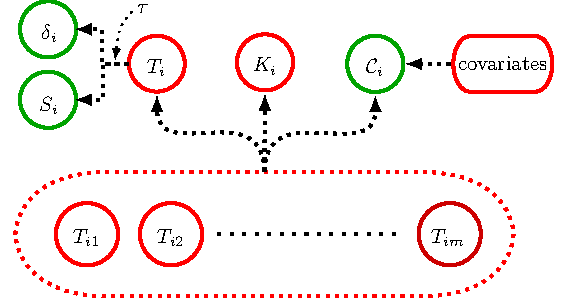
\includegraphics{./image/dep_model_standalone.pdf}

Figure 1: This figure showcases a dependency graph of the generative model for \(D_i = (S_i, \delta_i, \mathcal{C}_i)\). The elements in green are observed in the sample, while the elements in red are unobserved (latent). We see that \(\mathcal{C}_i\) is related to both the unobserved component lifetimes \(T_{i1},\ldots,T_{im}\) and other unknown and unobserved covariates, like ambient temperature or the particular diagnostician who generated the candidate set. These two complications for \(\mathcal{C}_i\) are why we seek a way to construct a reduced likelihood function in later sections that does not need to model the distribution of \(\mathcal{C}_i\).

An example of masked data \(D\) with a right-censoring time \(\tau = 5\) can be seen in Table 1
for a series system with \(3\) components.

\begin{longtable}[]{@{}llll@{}}
\caption{Right-censored lifetime data with masked component cause of failure.}\tabularnewline
\toprule
\begin{minipage}[b]{0.06\columnwidth}\raggedright
System\strut
\end{minipage} & \begin{minipage}[b]{0.32\columnwidth}\raggedright
Right-censored lifetime (\(S_i\))\strut
\end{minipage} & \begin{minipage}[b]{0.28\columnwidth}\raggedright
Event indicator (\(\delta_i\))\strut
\end{minipage} & \begin{minipage}[b]{0.22\columnwidth}\raggedright
Candidate set (\(\mathcal{C}_i\))\strut
\end{minipage}\tabularnewline
\midrule
\endfirsthead
\toprule
\begin{minipage}[b]{0.06\columnwidth}\raggedright
System\strut
\end{minipage} & \begin{minipage}[b]{0.32\columnwidth}\raggedright
Right-censored lifetime (\(S_i\))\strut
\end{minipage} & \begin{minipage}[b]{0.28\columnwidth}\raggedright
Event indicator (\(\delta_i\))\strut
\end{minipage} & \begin{minipage}[b]{0.22\columnwidth}\raggedright
Candidate set (\(\mathcal{C}_i\))\strut
\end{minipage}\tabularnewline
\midrule
\endhead
\begin{minipage}[t]{0.06\columnwidth}\raggedright
1\strut
\end{minipage} & \begin{minipage}[t]{0.32\columnwidth}\raggedright
\(1.1\)\strut
\end{minipage} & \begin{minipage}[t]{0.28\columnwidth}\raggedright
1\strut
\end{minipage} & \begin{minipage}[t]{0.22\columnwidth}\raggedright
\(\{1,2\}\)\strut
\end{minipage}\tabularnewline
\begin{minipage}[t]{0.06\columnwidth}\raggedright
2\strut
\end{minipage} & \begin{minipage}[t]{0.32\columnwidth}\raggedright
\(1.3\)\strut
\end{minipage} & \begin{minipage}[t]{0.28\columnwidth}\raggedright
1\strut
\end{minipage} & \begin{minipage}[t]{0.22\columnwidth}\raggedright
\(\{2\}\)\strut
\end{minipage}\tabularnewline
\begin{minipage}[t]{0.06\columnwidth}\raggedright
4\strut
\end{minipage} & \begin{minipage}[t]{0.32\columnwidth}\raggedright
\(2.6\)\strut
\end{minipage} & \begin{minipage}[t]{0.28\columnwidth}\raggedright
1\strut
\end{minipage} & \begin{minipage}[t]{0.22\columnwidth}\raggedright
\(\{2,3\}\)\strut
\end{minipage}\tabularnewline
\begin{minipage}[t]{0.06\columnwidth}\raggedright
5\strut
\end{minipage} & \begin{minipage}[t]{0.32\columnwidth}\raggedright
\(3.7\)\strut
\end{minipage} & \begin{minipage}[t]{0.28\columnwidth}\raggedright
1\strut
\end{minipage} & \begin{minipage}[t]{0.22\columnwidth}\raggedright
\(\{1,2,3\}\)\strut
\end{minipage}\tabularnewline
\begin{minipage}[t]{0.06\columnwidth}\raggedright
6\strut
\end{minipage} & \begin{minipage}[t]{0.32\columnwidth}\raggedright
\(5\)\strut
\end{minipage} & \begin{minipage}[t]{0.28\columnwidth}\raggedright
0\strut
\end{minipage} & \begin{minipage}[t]{0.22\columnwidth}\raggedright
\(\emptyset\)\strut
\end{minipage}\tabularnewline
\begin{minipage}[t]{0.06\columnwidth}\raggedright
3\strut
\end{minipage} & \begin{minipage}[t]{0.32\columnwidth}\raggedright
\(5\)\strut
\end{minipage} & \begin{minipage}[t]{0.28\columnwidth}\raggedright
0\strut
\end{minipage} & \begin{minipage}[t]{0.22\columnwidth}\raggedright
\(\emptyset\)\strut
\end{minipage}\tabularnewline
\bottomrule
\end{longtable}

In our model, we assume the data is governed by a pdf, which is determined by
a specific parameter, represented as \(\boldsymbol{\theta}\) within the parameter space \(\boldsymbol{\Omega}\).
The joint pdf of the data \(D\) can be represented as follows:
\[
f(D ; \boldsymbol{\theta}) = \prod_{i=1}^n f(D_i;\boldsymbol{\theta}) = \prod_{i=1}^n f(s_i,\delta_i,c_i;\boldsymbol{\theta}),
\]
where \(s_i\) is the observed system lifetime, \(\delta_i\) is the observed event
indicator, and \(c_i\) is the observed candidate set of the \(i\)\textsuperscript{th} system.

This joint pdf tells us how likely we are to observe the particular data, \(D\), given
the parameter \(\boldsymbol{\theta}\). When we keep the data constant and allow the parameter
\(\boldsymbol{\theta}\) to vary, we obtain what is called the likelihood function \(L\), defined as
\[
L(\boldsymbol{\theta}) = \prod_{i=1}^n L_i(\boldsymbol{\theta})
\]
where
\[
L_i(\boldsymbol{\theta}) = f(D_i;\boldsymbol{\theta})
\]
is the likelihood contribution of the \(i\)\textsuperscript{th} system.

For each type of data, right-censored data and masked component cause of
failure data, we will derive the \emph{likelihood contribution} \(L_i\), which refers
to the part of the likelihood function that this particular piece of data
contributes to. We present the following theorem for the likelihood contribution
model.

\begin{theorem}
\protect\hypertarget{thm:likelihood-contribution}{}\label{thm:likelihood-contribution}The likelihood contribution of the \(i\)\textsuperscript{th} system is given by
\begin{equation}
\label{eq:like}
L_i(\boldsymbol{\theta}) \propto \prod_{j=1}^m R_j(s_i;\boldsymbol{\theta_j}) \biggl(\sum_{j \in c_i} h_j(s_i;\boldsymbol{\theta_j}) \biggr)^{\delta_i}
\end{equation}
where \(\delta_i = 0\) indicates the \(i\)\textsuperscript{th} system is
right-censored at time \(s_i\) and \(\delta_i = 1\) indicates the \(i\)\textsuperscript{th} system
is observed to have failed at time \(s_i\) with a component cause of failure potentially masked
by the candidate set \(c_i\).
\end{theorem}

In the following subsections, we prove this result for each type of masked data,
right-censored system lifetime data \((\delta_i = 0)\) and masking of the
component cause of failure \((\delta_i = 1)\).

\hypertarget{candmod}{%
\subsection{Masked Component Cause of Failure}\label{candmod}}

When a system failure occurs, two types of data are observed in our data model:
the system's lifetime and a candidate set that is indicative of
the component cause of failure without necessarily precisely identifying the
failed component. This kind of masking of the true cause of failure is
especially prevalent in industrial settings. We will revisit this idea with a
real-world example to demonstrate its significance after introducing some
specific theoretical conditions.

The key goal of our analysis is to estimate the parameter \(\boldsymbol{\theta}\), which
maximizes the likelihood of the observed data, and to estimate the precision and
accuracy of this estimate using the Bootstrap method. To achieve this, we first
need to assess the joint distribution of the system's continuous lifetime,
\(T_i\), and the discrete candidate set, \(\mathcal{C}_i\), which can be written as
\[
f_{T_i,\mathcal{C}_i}(t_i,c_i;\boldsymbol{\theta}) = f_{T_i}(t_i;\boldsymbol{\theta})
    \Pr{}_{\!\boldsymbol{\theta}}\{\mathcal{C}_i = c_i | T_i = t_i\},
\]
where \(f_{T_i}(t_i;\boldsymbol{\theta})\) is the pdf of \(T_i\) and
\(\Pr{}_{\!\boldsymbol{\theta}}\{\mathcal{C}_i = c_i | T_i = t_i\}\) is the conditional
pmf of \(\mathcal{C}_i\) given \(T_i = t_i\).

We assume the pdf \(f_{T_i}(t_i;\boldsymbol{\theta})\) is known, but we do not have knowledge
of \(\Pr{}_{\!\boldsymbol{\theta}}\{\mathcal{C}_i = c_i | T_i = t_i\}\), i.e., the data generating
process for candidate sets is unknown. However, it is critical that the masked
data, \(\mathcal{C}_i\), is correlated with the \(i\)\textsuperscript{th} system.
This way, the conditional distribution of \(\mathcal{C}_i\) given \(T_i = t_i\) may
provide information about \(\boldsymbol{\theta}\), despite our statistical interest being
primarily in the series system rather than the candidate sets.

To make this problem tractable, we assume a set of conditions that make it
unnecessary to estimate the generative processes for candidate sets.
The most important way in which \(\mathcal{C}_i\) is correlated with the
\(i\)\textsuperscript{th} system is given by assuming the following condition.

\begin{condition}
\label{cond:c-contains-k}
The candidate set $\mathcal{C}_i$ contains the index of the failed component, i.e.,
$$
\Pr{}_{\!\boldsymbol{\theta}}\{K_i \in \mathcal{C}_i\} = 1,
$$
where $K_i$ is the random variable for the failed component index of the
$i$\textsuperscript{th} system.
\end{condition}

Assuming Condition \ref{cond:c-contains-k}, \(\mathcal{C}_i\) must contain the
index of the failed component, but we can say little else about what other
component indices may appear in \(\mathcal{C}_i\).
In order to derive the joint distribution of \(\mathcal{C}_i\) and \(T_i\) assuming
Condition \ref{cond:c-contains-k}, we take the following approach.
We notice that \(\mathcal{C}_i\) and \(K_i\) are statistically dependent.
We denote the conditional pmf of \(\mathcal{C}_i\) given \(T_i = t_i\) and
\(K_i = j\) as
\[
\Pr{}_{\!\boldsymbol{\theta}}\{\mathcal{C}_i = c_i | T_i = t_i, K_i = j\}.
\]

Even though \(K_i\) is not observable in our masked data model, we can still
consider the joint distribution of \(T_i\), \(K_i\), and \(\mathcal{C}_i\).
By Theorem \ref{thm:f-k-and-t}, the joint pdf of \(T_i\) and \(K_i\) is given by
\[
f_{T_i,K_i}(t_i,j;\boldsymbol{\theta}) = h_j(t_i;\boldsymbol{\theta_j}) \prod_{l=1}^m R_l(t_i;\boldsymbol{\theta_l}),
\]
where \(h_j(t_i;\boldsymbol{\theta_j})\) and \(R_j(s_i;\boldsymbol{\theta_j})\) are respectively the hazard
and reliability functions of the \(j\)\textsuperscript{th} component.
Thus, the joint pdf of \(T_i\), \(K_i\), and \(\mathcal{C}_i\) may be written as
\begin{equation}
\label{eq:joint-pdf-t-k-c}
\begin{split}
f_{T_i,K_i,\mathcal{C}_i}(t_i,j,c_i;\boldsymbol{\theta})
    &= f_{T_i,K_i}(t_i,k;\boldsymbol{\theta}) \Pr{}_{\!\boldsymbol{\theta}}\{\mathcal{C}_i=c_i|T_i=t_i,K_i=j\}\\
    &= h_j(t_i;\boldsymbol{\theta_j}) \prod_{l=1}^m R_l(t_i;\boldsymbol{\theta_l})
    \Pr{}_{\!\boldsymbol{\theta}}\{\mathcal{C}_i=c_i|T_i=t_i,K_i=j\}.
\end{split}
\end{equation}
We are going to need the joint pdf of \(T_i\) and \(\mathcal{C}_i\), which
may be obtained by summing over the support \(\{1,\ldots,m\}\) of \(K_i\) in
Equation \eqref{eq:joint-pdf-t-k-c},
\[
f_{T_i,\mathcal{C}_i}(t_i,c_i;\boldsymbol{\theta}) = \prod_{l=1}^m R_l(t_i;\boldsymbol{\theta_l})
    \sum_{j=1}^m \biggl\{
        h_j(t_i;\boldsymbol{\theta_j}) \Pr{}_{\!\boldsymbol{\theta}}\{\mathcal{C}_i=c_i|T_i=t_i,K_i=j\}
    \biggr\}.
\]
By Condition \ref{cond:c-contains-k},
\(\Pr{}_{\!\boldsymbol{\theta}}\{\mathcal{C}_i=c_i|T_i=t_i,K_i=j\} = 0\) when \(K_i = j\) and
\(j \notin c_i\), and so we may rewrite the joint pdf of \(T_i\) and
\(\mathcal{C}_i\) as
\begin{equation}
\label{eq:part1}
f_{T_i,\mathcal{C}_i}(t_i,c_i;\boldsymbol{\theta}) = \prod_{l=1}^m R_l(t_i;\boldsymbol{\theta_l})
    \sum_{j \in c_i} \biggl\{
        h_j(t_i;\boldsymbol{\theta_j}) \Pr{}_{\!\boldsymbol{\theta}}\{\mathcal{C}_i=c_i|T_i=t_i,K_i=j\}
    \biggr\}.
\end{equation}

When we try to find an MLE of \(\boldsymbol{\theta}\) (see Section \ref{mle}), we
solve the simultaneous equations of the MLE and choose a solution
\(\hat{\boldsymbol{\theta}}\) that is a maximum for the likelihood function.
When we do this, we find that \(\hat{\boldsymbol{\theta}}\) depends on the unknown
conditional pmf \(\Pr{}_{\!\boldsymbol{\theta}}\{\mathcal{C}_i=c_i|T_i=t_i,K_i=j\}\).
So, we are motivated to seek out more conditions (that approximately hold in
realistic situations) whose MLEs are independent of the pmf
\(\Pr{}_{\!\boldsymbol{\theta}}\{\mathcal{C}_i=c_i|T_i=t_i,K_i=j\}\).

\begin{condition}
\label{cond:equal-prob-failure-cause}
Given an observed system failure time $T_i=t_i$ and candidate set $c_i$,
the probability of the candidate set is the same when we condition on any
component cause of failure in the candidate set. That is,
$$
\Pr{}_{\!\boldsymbol{\theta}}\{\mathcal{C}_i=c_i|T_i=t_i,K_i=j'\} =
    \Pr{}_{\!\boldsymbol{\theta}}\{\mathcal{C}_i=c_i|T_i=t_i,K_i=j\}
$$
for all $j, j' \in c_i$.
\end{condition}

Assuming Conditions \ref{cond:c-contains-k} and
\ref{cond:equal-prob-failure-cause},
\(\Pr{}_{\!\boldsymbol{\theta}}\{\mathcal{C}_i=c_i|T_i=t_i,K_i=j\}\) may be factored out of the
summation in Equation \eqref{eq:part1}, and thus the joint pdf of \(T_i\) and
\(\mathcal{C}_i\) may be rewritten as
\[
f_{T_i,\mathcal{C}_i}(t_i,c_i;\boldsymbol{\theta}) =
    \Pr{}_{\!\boldsymbol{\theta}}\{\mathcal{C}_i=c_i|T_i=t_i,K_i=j'\} \prod_{l=1}^m R_l(t_i;\boldsymbol{\theta_l})
    \sum_{j \in c_i} h_j(t_i;\boldsymbol{\theta_j})
\]
where \(j' \in c_i\).

If \(\Pr{}_{\!\boldsymbol{\theta}}\{\mathcal{C}_i=c_i|T_i=t_i,K_i=j'\}\) is a function of
\(\boldsymbol{\theta}\), the MLEs are still dependent on the unknown
\(\Pr{}_{\!\boldsymbol{\theta}}\{\mathcal{C}_i=c_i|T_i=t_i,K_i=j'\}\).
This is a more tractable problem, but we are primarily interested in the
situation where we do not need to know or estimate
\(\Pr{}_{\!\boldsymbol{\theta}}\{\mathcal{C}_i=c_i|T_i=t_i,K_i=j'\}\) to find an MLE of
\(\boldsymbol{\theta}\). The last condition we assume achieves this result.

\begin{condition}
\label{cond:masked-indept-theta}
The masking probabilities conditioned on failure time $T_i$ and component cause
of failure $K_i$ are not functions of $\boldsymbol{\theta}$. In this case, the conditional
probability of $\mathcal{C}_i$ given $T_i=t_i$ and $K_i=j'$ is denoted by
$$
\beta_i = \Pr\{\mathcal{C}_i=c_i | T_i=t_i, K_i=j'\},
$$
where $\beta_i$ is not a function of $\boldsymbol{\theta}$.
\end{condition}

\hypertarget{real-world-relevance}{%
\subsubsection*{Real-World Relevance}\label{real-world-relevance}}
\addcontentsline{toc}{subsubsection}{Real-World Relevance}

According to \citep{Fran-1991}, many industrial problems feature masking due to time
constraints and the high costs associated with failure analysis. Crucially,
these industrial scenarios often fulfill Conditions \ref{cond:c-contains-k},
\ref{cond:equal-prob-failure-cause}, and \ref{cond:masked-indept-theta},
reinforcing the applicability of the results presented in this paper.

To elucidate, let's consider a diagnostic tool used for identifying failed components in an electronic device comprising three critical components
arranged in a series configuration. Two are on a common circuit board (labeled \(1\) and
\(2\)), while the third (labeled \(3\)) is separate.
Our diagnostic tool isolates the failure to either the circuit board or
the individual component but does not differentiate between components \(1\) and \(2\)
if the failure is on the shared board. In this case, we have the following
conditional probabilities for candidate sets:
\[
\Pr\{\mathcal{C}_i = c_i | T_i = t_i, K_i = j\}
\begin{cases}
  1 & \text{if $c_i = \{1,2\}$ and $j = 1$ or $j = 2$,}\\
  1 & \text{if $c_i = \{3\}$   and $j = 3$,}\\
  0 & \text{otherwise.}
\end{cases}
\]

Our diagnostic tool satisfies the conditions as follows:

\begin{itemize}
\item
  \textbf{Condition \ref{cond:c-contains-k}}: The candidate set \(c_i\) always
  contains the failed component \(j\). Our diagnostic tool is able to isolate the
  failure to either the circuit board or the individual component, and so the
  candidate set always contains the failed component.
\item
  \textbf{Condition \ref{cond:equal-prob-failure-cause}}: As we vary the cause of
  failure \(j\), we see that the conditional probability of the given candidate set \(c_i\) is the
  same for all \(j \in c_i\). Our diagnostic tool cannot distinguish between
  components \(1\) and \(2\) if the shared circuit board is the cause of failure, and
  therefore the probability of the candidate set is the same when we condition on
  either component \(1\) or \(2\) being the cause of failure.
\item
  \textbf{Condition \ref{cond:masked-indept-theta}}: The probabilities associated
  with our diagnostic tool are fixed and do not depend on the system parameter
  \(\boldsymbol{\theta}\).
\end{itemize}

By emphasizing that these conditions hold both in a general industrial context
and a specific real-world example, the paper enhances its applicability and
relevance to both theoreticians and practitioners.

\hypertarget{likelihood-contribution}{%
\subsubsection*{Likelihood Contribution}\label{likelihood-contribution}}
\addcontentsline{toc}{subsubsection}{Likelihood Contribution}

When Conditions \ref{cond:c-contains-k}, \ref{cond:equal-prob-failure-cause},
and \ref{cond:masked-indept-theta} are satisfied, the joint pdf of \(T_i\) and
\(\mathcal{C}_i\) is given by
\[
f_{T_i,\mathcal{C}_i}(t_i,c_i;\boldsymbol{\theta}) =
    \beta_i \prod_{l=1}^m R_l(t_i;\boldsymbol{\theta_l})
    \sum_{j \in c_i} h_j(t_i;\boldsymbol{\theta_j}).
\]
When we fix the sample and allow \(\boldsymbol{\theta}\) to vary, we obtain the
contribution to the likelihood \(L\) from the \(i\)\textsuperscript{th} observation
when the system lifetime is exactly known (\(\delta_i = 1\)) but the
component cause of failure is masked by a candidate set \(c_i\):
\begin{equation}
\label{eq:likelihood-contribution-masked}
L_i(\boldsymbol{\theta}) \propto \prod_{l=1}^m R_l(t_i;\boldsymbol{\theta_l})
    \sum_{j \in c_i} h_j(t_i;\boldsymbol{\theta_j}),
\end{equation}
where we dropped the factor \(\beta_i\) since it is not a function of \(\boldsymbol{\theta}\).\footnote{When doing maximum likelihood estimation, we are interested in the
  parameter values that maximize the likelihood function. Since \(\beta_i\) is not
  a function of \(\boldsymbol{\theta}\), it does not affect the location of the maximum of the
  likelihood function, and so we can drop it from the likelihood function.}

To summarize this result, assuming Conditions \ref{cond:c-contains-k},
\ref{cond:equal-prob-failure-cause}, and \ref{cond:masked-indept-theta},
if we observe an exact system failure time for the \(i\)\textsuperscript{th}
system (\(\delta_i = 1\)), but the component that failed is masked by a
candidate set \(c_i\), then its likelihood contribution is given by Equation
\eqref{eq:likelihood-contribution-masked}.

\hypertarget{right-censored-data}{%
\subsection{Right-Censored Data}\label{right-censored-data}}

As described in Section \ref{like-model}, we observe realizations of
\((S_i,\delta_i,\mathcal{C}_i)\) where \(S_i = \min\{T_i,\tau_i\}\) is the
right-censored system lifetime, \(\delta_i = 1_{T_i < \tau_i}\) is
the event indicator, and \(\mathcal{C}_i\) is the candidate set.

In the previous section, we discussed the likelihood contribution from an
observation of a masked component cause of failure, i.e., \(\delta_i = 1\).
We now derive the likelihood contribution of a \emph{right-censored} observation,
\(\delta_i = 0\), in our masked data model.

\begin{theorem}
\protect\hypertarget{thm:joint_s_d_c}{}\label{thm:joint_s_d_c}The likelihood contribution of a right-censored observation \((\delta_i = 0)\)
is given by
\begin{equation}
L_i(\boldsymbol{\theta}) = \prod_{l=1}^m R_l(s_i;\boldsymbol{\theta_l}).
\end{equation}
\end{theorem}

\begin{proof}
When right-censoring occurs, then \(S_i = \tau_i = s_i\), and we only know that
\(T_i > s_i\), and so we integrate over all possible values that it may have
obtained,
\[
L_i(\boldsymbol{\theta}) = \Pr\!{}_{\boldsymbol{\theta}}\{T_i > s_i\}.
\]
By definition, this is just the survival or reliability function of the series system
evaluated at \(s_i\),
\[
L_i(\boldsymbol{\theta}) = R_{T_i}(s_i;\boldsymbol{\theta}) = \prod_{l=1}^m R_l(s_i;\boldsymbol{\theta_l}).
\]
\end{proof}

When we combine the two likelihood contributions, we obtain the likelihood
contribution for the \(i\)\textsuperscript{th} system shown in Theorem
\ref{thm:likelihood-contribution},
\[
L_i(\boldsymbol{\theta}) \propto
\begin{cases}
    \prod_{l=1}^m R_l(s_i;\boldsymbol{\theta_l})         &\text{ if } \delta_i = 0\\
    \prod_{l=1}^m R_l(s_i;\boldsymbol{\theta_l})
        \sum_{j\in c_i} h_j(s_i;\boldsymbol{\theta_j})   &\text{ if } \delta_i = 1.
\end{cases}
\]
We use this result in Section \ref{mle} to derive the maximum likelihood
estimator (MLE) of \(\boldsymbol{\theta}\).

\hypertarget{identifiability}{%
\subsection{Identifiability and Convergence Issues}\label{identifiability}}

In our likelihood model, masking and right-censoring can lead to issues related
to identifiability and flat likelihood regions.
Identifiability refers to the unique mapping of the model parameters to the
likelihood function, and lack of identifiability can lead
to multiple sets of parameters that explain the data equally well, making inference
about the true parameters challenging \citep{lehmann1998theory}, while
flat likelihood regions can complicate convergence \citep{wu1983convergence}.

In our simulation study, we address these challenges in a pragmatic way. Specifically,
failure to converge to a solution within a maximum of 125 iterations is interpreted as
evidence of the aforementioned issues, leading to the discarding of the sample.\footnote{The choice of 125 iterations was also made for practical reasons.
  Since we are generating millions of samples and trying to find an MLE for
  each in our simulation study, if we did not limit the number of iterations, the
  simulation study would have taken too long to run.}
However, in Section \ref{boot}, where we discuss the bias-corrected and
accelerated (BCa) bootstrap method for constructing confidence intervals, we
do not discard any resamples. This strategy helps ensure the robustness of the
results, while acknowledging the inherent complexities of likelihood-based
estimation in models characterized by masking and right-censoring. In our
simulation study, we report the convergence rates, and find that for most
scenarios, the convergence rate is greater than \(95\%\) (\(100\%\) once
the sample is sufficiently large).

\hypertarget{mle}{%
\section{Maximum Likelihood Estimation}\label{mle}}

In our analysis, we use maximum likelihood estimation (MLE) to estimate the series
system parameter \(\boldsymbol{\theta}\) from the masked data \citep{bain1992, casella2002statistical}.
The MLE finds parameter values that maximize the likelihood of the observed data
under the assumed model. A maximum likelihood estimate, \(\hat{\boldsymbol{\theta}}\), is a
solution of
\begin{equation}
\label{eq:mle}
L(\hat{\boldsymbol{\theta}}) = \max_{\boldsymbol{\theta }\in \boldsymbol{\Omega}} L(\boldsymbol{\theta}),
\end{equation}
where \(L(\boldsymbol{\theta})\) is the likelihood function of the observed data. For computational
efficiency and analytical simplicity, we work with the log-likelihood function,
denoted as \(\ell(\boldsymbol{\theta})\), instead of the likelihood function \citep{casella2002statistical}.

\begin{theorem}
\protect\hypertarget{thm:loglike-total}{}\label{thm:loglike-total}The log-likelihood function, \(\ell(\boldsymbol{\theta})\), for our masked data model is the sum of the log-likelihoods for each observation,
\begin{equation}
\label{eq:loglike}
\ell(\boldsymbol{\theta}) = \sum_{i=1}^n \ell_i(\boldsymbol{\theta}),
\end{equation}
where \(\ell_i(\boldsymbol{\theta})\) is the log-likelihood contribution for the \(i\)\textsuperscript{th} observation:
\begin{equation}
\ell_i(\boldsymbol{\theta}) = \sum_{j=1}^m \log R_j(s_i;\boldsymbol{\theta_j}) +
    \delta_i \log \biggl(\sum_{j\in c_i} h_j(s_i;\boldsymbol{\theta_j}) \biggr).
\end{equation}
\end{theorem}

\begin{proof}
The log-likelihood function is the logarithm of the likelihood function,
\[
\ell(\boldsymbol{\theta}) = \log L(\boldsymbol{\theta}) = \log \prod_{i=1}^n L_i(\boldsymbol{\theta}) =
    \sum_{i=1}^n \log L_i(\boldsymbol{\theta}).
\]
Substituting \(L_i(\boldsymbol{\theta})\) from Equation \eqref{eq:like}, we consider these two
cases of \(\delta_i\) separately to obtain the result in Theorem
\ref{thm:loglike-total}.
\textbf{Case 1}: If the \(i\)\textsuperscript{th} system is right-censored (\(\delta_i = 0\)),
\[
\ell_i(\boldsymbol{\theta}) = \log \prod_{l=1}^m R_l(s_i;\boldsymbol{\theta_l}) =
    \sum_{l=1}^m \log R_l(s_i;\boldsymbol{\theta_l}).
\]
\textbf{Case 2}: If the \(i\)\textsuperscript{th} system's component cause of failure is masked but
the failure time is known (\(\delta_i = 1\)),
\[
\ell_i(\boldsymbol{\theta}) = \sum_{l=1}^m \log R_l(t_i;\boldsymbol{\theta_l}) + \log \beta_i +
    \log \biggl(\sum_{j\in c_i} h_j(s_i;\boldsymbol{\theta_j})\biggr).
\]
By Condition \ref{cond:masked-indept-theta},
we may discard the \(\log \beta_i\) term since it does not depend on \(\boldsymbol{\theta}\),
giving us the result
\[
\ell_i(\boldsymbol{\theta}) = \sum_{l=1}^m \log R_l(s_i;\boldsymbol{\theta_l}) +
    \log \biggl(\sum_{j\in c_i} h_j(s_i;\boldsymbol{\theta_j}) \biggr).
\]
Combining these two cases gives us the result in Theorem \ref{thm:loglike-total}.
\end{proof}

The MLE, \(\hat{\boldsymbol{\theta}}\), is often found by solving a system of equations
derived from setting the derivative of the log-likelihood function to zero
\citep{bain1992}, i.e.,
\begin{equation}
\label{eq:mle-eq}
\frac{\partial}{\partial \theta_j} \ell(\boldsymbol{\theta}) = 0,
\end{equation}
for each component \(\theta_j\) of the parameter \(\boldsymbol{\theta}\). When there's no
closed-form solution, we resort to numerical methods like the Newton-Raphson
method.

Assuming some regularity conditions, such as the likelihood function being
identifiable, the MLE has many desirable asymptotic properties that underpin
statistical inference, namely that it is an asymptotically unbiased estimator
of the parameter \(\boldsymbol{\theta}\) and it is normally distributed with a variance given
by the inverse of the Fisher Information Matrix (FIM) \citep{casella2002statistical}.
However, for smaller samples, these asymptotic properties may not yield accurate
approximations. We propose to use the bootstrap method to offer an empirical
approach for estimating the sampling distribution of the MLE, in particular for
computing confidence intervals.

\hypertarget{boot}{%
\section{Bias-Corrected and Accelerated Bootstrap Confidence Intervals}\label{boot}}

We utilize the non-parametric bootstrap to estimate the sampling distribution
of the MLE. In the non-parametric bootstrap, we resample from the observed data
with replacement to generate a bootstrap sample. The MLE is then computed for
the bootstrap sample. This process is repeated to generate numerous bootstrap
replicates of the MLE. The sampling distribution of the MLE is then estimated
by the empirical distribution of the bootstrap replicates of the MLE.

Our main focus is on generating confidence intervals for the MLE. The method we
use to generate confidence intervals is known as Bias-Corrected and Accelerated
Bootstrap Confidence Intervals (BCa) \citep{efron1987better}, which applies two
corrections to the standard bootstrap method:

\begin{itemize}
\item
  \textbf{Bias Correction}: This adjusts for bias in the bootstrap distribution itself.
  This bias is measured as the difference between the mean of the bootstrap
  distribution and the observed statistic. It works by transforming the
  percentiles of the bootstrap distribution to correct for these issues.\\
  This may be a useful adjustment in our case since we are dealing with
  small samples with two potential sources of bias: right-censoring and
  masking component cause of failure.
\item
  \textbf{Acceleration}: This adjusts for the rate of change of the statistic as a
  function of the true, unknown parameter. This correction is important when the
  shape of the statistic's distribution changes with the true parameter.
  Since we have a number of different shape parameters, \(k_1,\ldots,k_m\), we may
  expect the shape of the distribution of the MLE to change as a function of the
  true parameter, making this correction potentially useful.
\end{itemize}

\hypertarget{correctly-specified-confidence-intervals}{%
\paragraph*{Correctly Specified Confidence Intervals}\label{correctly-specified-confidence-intervals}}
\addcontentsline{toc}{paragraph}{Correctly Specified Confidence Intervals}

Since we are primarily interested in generating confidence intervals for small
samples for a biased MLE, the BCa method is a reasonable choice for our
simulation study. In our simulation study, we evaluate the performance of the
BCa confidence intervals by calculating their coverage probability. A \emph{correctly
specified} \(95\%\) confidence interval contains the true parameter value
approximately \(95\%\) of the time in repeated sampling.

In this study, we consider a coverage probability above \(90\%\) to be
satisfactory, as it offers a reasonable trade-off between precision and
reliability. A coverage probability below this would signify undue confidence in
the precision of the MLE. Conversely, a coverage probability near \(100\%\) may
indicate excessively wide intervals, thereby diminishing the precision of the
MLE. Our objective is to construct confidence intervals that are as narrow as
possible while achieving good empirical coverage close to the nominal level of
\(95\%\).

\hypertarget{challenges}{%
\subparagraph*{Challenges}\label{challenges}}
\addcontentsline{toc}{subparagraph}{Challenges}

While the bootstrap method provides a robust and flexible tool for statistical
estimation, its effectiveness can be influenced by many factors. A few of these
factors are particularly relevant to our study:

\begin{itemize}
\tightlist
\item
  \textbf{Convergence}: Instances of non-convergence in our bootstrap samples were
  observed, which can occur when the estimation method, like the MLE used in our
  analysis, fails to converge due to the specifics of the resampled data
  \citep{casella2002statistical}. This issue can potentially introduce bias or
  reduce the effective sample size of our bootstrap distribution.
\item
  \textbf{Small Samples}: The bootstrap's accuracy can be compromised with small
  sample sizes, as the method relies on the Law of Large Numbers to approximate
  the true sampling distribution. For small samples, the bootstrap resamples might
  not adequately represent the true variability in the data, leading to inaccurate
  results \citep{efron1994introduction}.
\item
  \textbf{Masking}: Our data involves right censoring and a masking of the component
  cause of failure when a system failure is observed. These aspects can cause
  certain data points or trends to be underrepresented or not represented at all
  in our data, introducing bias in the bootstrap distribution \citep{klein2005survival}.
\end{itemize}

Despite these challenges, we found the bootstrap method useful in constructing
correctly specified confidence intervals.

\hypertarget{weibull}{%
\section{Series System with Weibull Components}\label{weibull}}

The Weibull distribution, introduced by Waloddi Weibull in 1937, has been
instrumental in reliability analysis due to its ability to model a wide range
of failure behaviors. Reflecting on its utility, Weibull
modestly noted that it ``{[}\ldots{]} may sometimes render good service.'' \citep{Abernethy2006}
In the context of our study, we model a system as originating from components
with Weibull distributed lifetimes arranged in a series configuration,
producing a specific form of the likelihood model described in Section \ref{like-model},
which deals with challenges such as right censoring and masked component cause of failure.

The \(j\)\textsuperscript{th} component of the \(i\)\textsuperscript{th} system has a
lifetime distribution given by
\[
    T_{i j} \sim \operatorname{Weibull}(k_j,\lambda_j) \qquad \text{for } i = 1,\ldots,n \text{ and } j = 1,\ldots,m,
\]
where \(\lambda_j > 0\) is the scale parameter and \(k_j > 0\) is the shape parameter.
The \(j\)\textsuperscript{th} component has a reliability function, pdf, and hazard function
given respectively by
\begin{align}
    R_j(t;\lambda_j,k_j)
        &= \exp\biggl\{-\biggl(\frac{t}{\lambda_j}\biggr)^{k_j}\biggr\},\\
    f_j(t;\lambda_j,k_j)
        &= \frac{k_j}{\lambda_j}\biggl(\frac{t}{\lambda_j}\biggr)^{k_j-1}
        \exp\biggl\{-\left(\frac{t}{\lambda_j}\right)^{k_j} \biggr\},\\
    h_j(t;\lambda_j,k_j) \label{eq:weibull-haz}
        &= \frac{k_j}{\lambda_j}\biggl(\frac{t}{\lambda_j}\biggr)^{k_j-1}.
\end{align}

The shape parameter of the Weibull distribution is of particular importance:

\begin{itemize}
\tightlist
\item
  \(k_j < 1\) indicates infant mortality. An example of how this might arise is
  a result of defective components being weeded out early, and the remaining
  components surviving for a much longer time.
\item
  \(k_j = 1\) indicates random failures (independent of age). An example of how
  this might arise is a result of random shocks to the system, but otherwise
  the system is age-independent.\footnote{The exponential distribution is a special case of the Weibull distribution
    when \(k_j = 1\).}
\item
  \(k_j > 1\) indicates wear-out failures. An example of how this might arise is a
  result of components wearing as they age.
\end{itemize}

We show that the lifetime of the series system composed of \(m\) Weibull
components has a reliability, hazard, and probability density functions given by
the following theorem.

\begin{theorem}
\protect\hypertarget{thm:sys_weibull}{}\label{thm:sys_weibull}The lifetime of a series system composed of \(m\) Weibull components
has a reliability function, hazard function, and pdf respectively given by
\begin{align}
\label{eq:sys-weibull-reliability-fn}
R_{T_i}(t;\boldsymbol{\theta}) &= \exp\biggl\{-\sum_{j=1}^{m}\biggl(\frac{t}{\lambda_j}\biggr)^{k_j}\biggr\},\\
\label{eq:sys-weibull-failure-rate-fn}
h_{T_i}(t;\boldsymbol{\theta}) &= \sum_{j=1}^{m} \frac{k_j}{\lambda_j}\biggl(\frac{t}{\lambda_j}\biggr)^{k_j-1},\\
\label{eq:sys-weibull-pdf}
f_{T_i}(t;\boldsymbol{\theta}) &= \biggl\{
    \sum_{j=1}^m \frac{k_j}{\lambda_j}\left(\frac{t}{\lambda_j}\right)^{k_j-1}
\biggr\}
\exp
\biggl\{
    -\sum_{j=1}^m \bigl(\frac{t}{\lambda_j}\bigr)^{k_j}
\biggr\},
\end{align}
where \(\boldsymbol{\theta }= (k_1, \lambda_1, \ldots, k_m, \lambda_m)\) is the parameter
vector of the series system and \(\boldsymbol{\theta_j} = (k_j, \lambda_j)\) is the
parameter vector of the \(j\)\textsuperscript{th} component.
\end{theorem}

\begin{proof}
The proof for the reliability function follows from Theorem \ref{thm:sys-reliability-fn},
\[
R_{T_i}(t;\boldsymbol{\theta}) = \prod_{j=1}^{m} R_j(t;\lambda_j,k_j).
\]
Plugging in the Weibull component reliability functions obtains the result
\begin{align*}
R_{T_i}(t;\boldsymbol{\theta})
    = \prod_{j=1}^{m} \exp\biggl\{-\biggl(\frac{t}{\lambda_j}\biggr)^{k_j}\biggr\}
    = \exp\biggl\{-\sum_{j=1}^{m}\biggl(\frac{t}{\lambda_j}\biggr)^{k_j}\biggr\}.
\end{align*}
The proof for the hazard function follows from Theorem \ref{thm:sys-failure-rate},
\begin{align*}
h_{T_i}(t;\boldsymbol{\theta})
    = \sum_{j=1}^{m} h_j(t;\boldsymbol{\theta_j})
    = \sum_{j=1}^{m} \frac{k_j}{\lambda_j}\biggl(\frac{t}{\lambda_j}\biggr)^{k_j-1}.
\end{align*}
The proof for the pdf follows from Theorem \ref{thm:sys-pdf}. By definition,
\[
f_{T_i}(t;\boldsymbol{\theta}) = h_{T_i}(t;\boldsymbol{\theta}) R_{T_i}(t;\boldsymbol{\theta}).
\]
Plugging in the failure rate and reliability functions given respectively by
Equations \eqref{eq:sys-weibull-reliability-fn} and
\eqref{eq:sys-weibull-failure-rate-fn} completes the proof.
\end{proof}

In Section \ref{reliability}, we discussed the concept of reliability, with
the MTTF being a common measure of reliability. In the case of Weibull
components, the MTTF of the \(j\)\textsuperscript{th} component is given by
\begin{equation}
\label{eq:mttf-weibull}
\text{MTTF}_j = \lambda_j \Gamma\biggl(1 + \frac{1}{k_j}\biggr),
\end{equation}
where \(\Gamma\) is the gamma function. We mentioned that the MTTF can sometimes
be a poor measure of reliability, e.g., the MTTF and the probability of failing
early can \emph{both} be large. The Weibull is a good example of this phenomenon.
If \(k_j > 1\), the lifetime distribution of the \(j\)\textsuperscript{th} component
is fat-tailed and it can exhibit both a large MTTF and a high probability of
failing early. The probability of component failure given by Equation
\eqref{eq:prob-k} is a particularly useful measure of component reliability
relative to the other components in the system.

\hypertarget{sys-weibull-like}{%
\subsection{Likelihood Model}\label{sys-weibull-like}}

In Section \ref{like-model}, we discussed two separate kinds of likelihood
contributions, masked component cause of failure data (with exact system failure
times) and right-censored data. The likelihood contribution of the
\(i\)\textsuperscript{th} system is given by the following theorem.

\begin{theorem}
\protect\hypertarget{thm:weibull-likelihood-contribution}{}\label{thm:weibull-likelihood-contribution}Let \(\delta_i\) be an indicator variable that is 1 if the
\(i\)\textsuperscript{th} system fails and 0 (right-censored) otherwise.
Then the likelihood contribution of the \(i\)\textsuperscript{th} system is given by
\begin{equation}
\label{eq:weibull-likelihood-contribution}
L_i(\boldsymbol{\theta}) \propto
\begin{cases}
    \exp\biggl\{-\sum_{j=1}^{m}\bigl(\frac{t_i}{\lambda_j}\bigr)^{k_j}\biggr\}
        \sum_{j \in c_i} \frac{k_j}{\lambda_j}\bigl(\frac{t_i}{\lambda_j}\bigr)^{k_j-1}
    & \text{if } \delta_i = 1,\\
    \exp\bigl\{-\sum_{j=1}^{m}\bigl(\frac{t_i}{\lambda_j}\bigr)^{k_j}\biggr\} & \text{if } \delta_i = 0.
\end{cases}
\end{equation}
\end{theorem}

\begin{proof}
By Theorem \ref{thm:likelihood-contribution}, the likelihood contribution of the
\(i\)\textsuperscript{th} system is given by
\[
L_i(\boldsymbol{\theta}) \propto
\begin{cases}
    R_{T_i}(s_i;\boldsymbol{\theta})                       &\text{ if } \delta_i = 0\\
    R_{T_i}(s_i;\boldsymbol{\theta})
        \sum_{j\in c_i} h_j(s_i;\boldsymbol{\theta_j})   &\text{ if } \delta_i = 1.
\end{cases}
\]
By Equation \eqref{eq:sys-weibull-reliability-fn}, the system reliability
function is given by
\[
R_{T_i}(t_i;\boldsymbol{\theta}) = \exp\biggl\{-\sum_{j=1}^{m}\biggl(\frac{t_i}{\lambda_j}\biggr)^{k_j}\biggr\},
\]
where \(\boldsymbol{\theta }= (k_1,\lambda_1,\ldots,k_m,\lambda_m)\) is the parameter vector and by
Equation \eqref{eq:weibull-haz}, the hazard function of the \(j\)\textsuperscript{th}
component is given by
\[
h_j(t_i;\boldsymbol{\theta_j}) = \frac{k_j}{\lambda_j}\biggl(\frac{t_i}{\lambda_j}\biggr)^{k_j-1},
\]
where \(\boldsymbol{\theta_j} = (k_j,\lambda_j)\) is the parameter vector of the
\(j\)\textsuperscript{th} component. Plugging these into the likelihood contribution
function obtains the result.
\end{proof}

Taking the log of the likelihood contribution function obtains the following result.

\begin{corollary}
\protect\hypertarget{cor:cor:weibull-log-likelihood-contribution}{}\label{cor:cor:weibull-log-likelihood-contribution}The log-likelihood contribution of the \(i\)\textsuperscript{th} system is given by
\begin{equation}
\label{eq:weibull-log-likelihood-contribution}
\ell_i(\boldsymbol{\theta}) =
-\sum_{j=1}^{m}\biggl(\frac{t_i}{\lambda_j}\biggr)^{k_j} +
    \delta_i \log \!\Biggl(    
        \sum_{j \in c_i} \frac{k_j}{\lambda_j}\biggl(\frac{t_i}{\lambda_j}\biggr)^{k_j-1}
    \Biggr)
\end{equation}
where we drop any terms that do not depend on \(\boldsymbol{\theta}\) since they do not
affect the MLE.
\end{corollary}

See Appendix \ref{app-weibull-loglik-r} for the R code that implements the log-likelihood function
for the series system with Weibull components.

We find an MLE by solving \eqref{eq:mle-eq}, i.e., a point
\(\boldsymbol{\hat\theta} = (\hat{k}_1,\hat{\lambda}_1,\ldots,\hat{k}_m,\hat{\lambda}_m)\)
satisfying \(\nabla_{\boldsymbol{\theta}} \ell(\boldsymbol{\hat{\boldsymbol{\theta}}}) = \boldsymbol{0}\), where
\(\nabla_{\boldsymbol{\theta}} \ell\) is the gradient of the log-likelihood function (score) with
respect to \(\boldsymbol{\theta}\). To solve this system of equations, we use Newton-like
methods, which sometimes require both the gradient and the Hessian of the
log-likelihood function. We analytically derive the score but we do not do the
same for the Hessian of the log-likelihood function. Our reasoning is based on
the following two observations:

\begin{itemize}
\item
  The score function is relatively easy to derive, and it is useful to have for
  computing gradients efficiently and accurately, which will be useful for
  accurately numerically approximating the Hessian of the log-likelihood function.
\item
  The Hessian is tedious and error prone to derive, and Newton-like methods
  often do not require the Hessian to be explicitly computed.
\end{itemize}

The following theorem derives the score function.

\begin{theorem}
\protect\hypertarget{thm:weibull-score}{}\label{thm:weibull-score}The gradient of the log-likelihood contribution of the \(i\)\textsuperscript{th} system is given by
\begin{equation}
\label{eq:weibull-score}
\nabla \ell_i(\boldsymbol{\theta}) = \biggl(
    \frac{\partial \ell_i(\boldsymbol{\theta})}{\partial k_1},
    \frac{\partial \ell_i(\boldsymbol{\theta})}{\partial \lambda_1},
    \cdots, 
    \frac{\partial \ell_i(\boldsymbol{\theta})}{\partial k_m},
    \frac{\partial \ell_i(\boldsymbol{\theta})}{\partial \lambda_m} \biggr)',
\end{equation}
where
\begin{equation}
\frac{\partial \ell_i(\boldsymbol{\theta})}{\partial k_r} = 
    -\biggl(\frac{t_i}{\lambda_r}\biggr)^{k_r}    
        \!\!\log\biggl(\frac{t_i}{\lambda_r}\biggr) +
        \frac{\frac{1}{t_i} \bigl(\frac{t_i}{\lambda_r}\bigr)^{k_r}
            \bigl(1+ k_r \log\bigl(\frac{t_i}{\lambda_r}\bigr)\bigr)}
            {\sum_{j \in c_i} \frac{k_j}{\lambda_j}\bigl(\frac{t_i}{\lambda_j}\bigr)^{k_j-1}}
        1_{\delta_i = 1 \land r \in c_i}
\end{equation}
and
\begin{equation}
\frac{\partial \ell_i(\boldsymbol{\theta})}{\partial \lambda_r} = 
    \frac{k_r}{\lambda_r} \biggl(\frac{t_i}{\lambda_r}\biggr)^{k_r} -
    \frac{
        \bigl(\frac{k_r}{\lambda_r}\bigr)^2 \bigl(\frac{t_i}{\lambda_r}\bigr)^{k_r - 1}
    }
    {
        \sum_{j \in c_i} \frac{k_j}{\lambda_j}\bigl(\frac{t_i}{\lambda_j}\bigr)^{k_j-1}
    }
    1_{\delta_i = 1 \land r \in c_i}.
\end{equation}
\end{theorem}

The result follows from taking the partial derivatives of the log-likelihood
contribution of the \(i\)\textsuperscript{th} system given by Equation
\eqref{eq:weibull-likelihood-contribution}. It is a tedious calculation so the
proof has been omitted, but the result has been verified by using a very precise
numerical approximation of the gradient.

By the linearity of differentiation, the gradient of a sum of functions is
the sum of their gradients, and so the score function conditioned on the entire
sample is given by
\begin{equation}
\label{eq:weibull-series-score}
\nabla \ell(\boldsymbol{\theta}) = \sum_{i=1}^n \nabla \ell_i(\boldsymbol{\theta}).
\end{equation}

\hypertarget{reduced-weibull}{%
\subsection{Weibull Series System: Homogeneous Shape Parameters}\label{reduced-weibull}}

In a series system, the system is only as reliable as its weakest link
(weakest component). In a well-designed series system, there is no single
component that is much weaker than the others. In the case of components with
Weibull lifetimes, this implies the shape parameters are homogenous and the
scale parameters are homogenous. The shape parameters are particularly important
since they determine the failure behavior of the components.

When the shape parameters are homogenous, the lifetime of the series system with
components that are Weibull distributed is also Weibull distributed, as shown in
the following theorem.

\begin{theorem}
\protect\hypertarget{thm:weibull-series-system}{}\label{thm:weibull-series-system}If the shape parameters of the components are homogenous, then the lifetime
series system follows a Weibull distribution with a shape parameter \(k\) given by
the identical shape parameters of the components and a scale parameter \(\lambda\)
given by
\begin{equation}
\label{eq:sys-weibull-scale}
\lambda = \biggl(\sum_{j=1}^{m} \lambda_j^{-k}\biggr)^{-1/k},
\end{equation}
where \(\lambda_j\) is the scale parameter of the \(j\)\textsuperscript{th} component.
\end{theorem}

\begin{proof}
Given \(m\) Weibull lifetimes \(T_{i 1}, \ldots, T_{i m}\) with the same shape
parameter \(k\) and scale parameters \(\lambda_1, \ldots, \lambda_m\), the
reliability function of the series system is given by
\[
R_{T_i}(t;\boldsymbol{\theta}) =
    \exp\biggl\{-\sum_{j=1}^{m}\biggl(\frac{t}{\lambda_j}\biggr)^{k}\biggr\}.
\]
To show that the series system lifetime is Weibull, we need to find a single
scale parameter \(\lambda\) such that
\[
R_{T_i}(t;\boldsymbol{\theta}) = \exp\biggl\{-\biggl(\frac{t}{\lambda}\biggr)^{k}\biggr\},
\]
which has the solution
\[
\lambda = \frac{1}{\left(\frac{1}{\lambda_1^k} + \ldots +
    \frac{1}{\lambda_m^k}\right)^{\frac{1}{k}}}.
\]
\end{proof}

\begin{theorem}
If a series system has Weibull components with homogeneous shape parameters, the
component cause of failure is conditionally independent of the system failure
time:
\[
\Pr\{K_i = j | T_i = t_i \} = \Pr\{K_i = j\} =
    \frac{\lambda_j^{-k}}{\sum_{l=1}^{m} \lambda_l^{-k}}.
\]
\end{theorem}

\begin{proof}
By Theorem \ref{thm:prob-k-given-t}, the conditional probability of the
\(j\)\textsuperscript{th} component being the cause of failure given the system
failure time is given by
\begin{align*}
\Pr\{K_i = j | T_i = t\}
    &= \frac{f_{K_i, T_i}(j, t;\boldsymbol{\theta})}{f_{T_i}(t;\boldsymbol{\theta})}
    = \frac{h_j(t;k,\lambda_j) R_{T_i}(t;\boldsymbol{\theta})}
        {h_{T_i}(t;\boldsymbol{\theta_j}) R_{T_i}(t;\boldsymbol{\theta})}\\
    &= \frac{h_j(t;k,\lambda_j)}{\sum_{l=1}^m h_l(t;k,\lambda_l)}
    = \frac{\frac{k}{\lambda_j}\bigl(\frac{t}{\lambda_j}\bigr)^{k-1}}
        {\sum_{l=1}^m \frac{k}{\lambda_l}\bigl(\frac{t}{\lambda_l}\bigr)^{k-1}}
    = \frac{\bigl(\frac{1}{\lambda_j}\bigr)^k}
        {\sum_{l=1}^m \bigl(\frac{1}{\lambda_l}\bigr)^k}.
\end{align*}
\end{proof}

According to the bias-variance trade-off, we expect the MLE of the homogenous
model, which has \(m+1\) parameters (\(m\) being he number of components in the
series system), to be more biased but have less variance than the MLE of the
full model, which has \(2m\) parameters.

\hypertarget{sim-study}{%
\section{Simulation Study: Series System with Weibull Components}\label{sim-study}}

In this simulation study, we assess the sensitivity of the MLE and BCa
confidence intervals to various simulation scenarios for the likelihood model
defined in Section \ref{weibull}. We begin by specifying the parameters of the
series system that will be the central object of our simulation study. We
consider the data in \citep{Huairu-2013}, in which they study the reliability of a
series system with three components. They fit Weibull components in a series
configuration to the data, resulting in an MLE with shape and scale estimates
given by the first three components in Table \ref{tab:series-sys}. To make the
model slightly more complex, we add two more components to this series system,
with shape and scale parameters given by the last two components in Table
\ref{tab:series-sys}. We will refer to this system as the \textbf{base} system.

In Section \ref{reliability}, we defined a well-designed series system as one
that consists of components with similar reliabilities, where we define
reliability in three ways: the reliability function, MTTF, and probability that
a specific component will be the cause of failure (which is a measure of
relative reliability of the components). We will use these three measures of
reliability to assess the base system. The base system
defined in Table \ref{tab:series-sys} satisfies this definition of being a
well-designed system since there are no components that are significantly
less reliable than any of the others, component 1 being the most reliable and
component 3 being the least reliable.

The reliability function, unlike the other two measures of reliability, is not
a summary statistic of reliability, but is rather a function of time. Since most
of our simulations have the right-censoring time set to the \(82.5\%\) quantile of
the series system, which we denote here by \(\tau_{0.825}\), we can compare the
reliability functions of the components at this time. We see that the
reliability of the components at this right-censoring time are similar, with
component 1 being the most reliable and component 3 being the least reliable.
These results are consistent with the previous analysis based on the MTTF and
probability of component cause of failure being similar.

The shape parameters for each component is larger than \(1\), which means each
component has a failure characteristic that is more wear-out than infant
mortality. The system as a whole is therefore more likely to fail due to
wear-out failures than infant mortality. This too is consistent with a
well-designed system.

\hypertarget{homogenous-shape-parameters}{%
\paragraph*{Homogenous Shape Parameters}\label{homogenous-shape-parameters}}
\addcontentsline{toc}{paragraph}{Homogenous Shape Parameters}

The base system is a well-designed system, and so it is likely that the
likelihood model that assumes homogeneous shape parameters described in Section
\ref{reduced-weibull} would provide a good fit to any data generated from this
system. We performed a preliminary investigation into this by simulating data
from the base system, and deviations from the base system that make the system
less well-designed, and fitting the homogeneous model to the data. We found that
the MLE of the homogeneous model was very close to the true parameter values for
slight deviations from the base system, but the MLE was biased for larger
deviations from the base system. This is consistent with the bias-variance
trade-off, where the MLE of the homogeneous model is more biased but has less
variance than the MLE of the full model. We do not explore this further in this
simulation study, but it is an interesting avenue for future research.

\begin{table}

\caption{\label{tab:series-sys}Weibull Components in Series Configuration}
\centering
\begin{tabular}[t]{l|r|r|r|r|r}
\hline
  & Shape ($k_j$) & Scale ($\lambda_j$) & MTTF$_j$ & $\Pr\{K_i = j\}$ & $R_j(\tau_{0.825};k_j,\lambda_j)$\\
\hline
Component 1 & 1.2576 & 994.3661 & 924.869 & 0.169 & 0.744\\
\hline
Component 2 & 1.1635 & 908.9458 & 862.157 & 0.207 & 0.698\\
\hline
Component 3 & 1.1308 & 840.1141 & 803.564 & 0.234 & 0.667\\
\hline
Component 4 & 1.1802 & 940.1342 & 888.237 & 0.196 & 0.711\\
\hline
Component 5 & 1.2034 & 923.1631 & 867.748 & 0.195 & 0.711\\
\hline
Series System & NA & NA & 222.884 & NA & 0.175\\
\hline
\end{tabular}
\end{table}

\hypertarget{performance-metrics}{%
\subsection{Performance Metrics}\label{performance-metrics}}

In this section, we describe the measures we use to assess the performance of
the MLE and the BCa confidence intervals in our simulation study. We assess two
important properties of the MLE for each simulation scenario:

\begin{itemize}
\item
  \textbf{Accuracy (Bias)}: A pivotal metric is the proximity of the MLE's expected
  value to the true parameter value. Higher accuracy is demonstrated by a
  closer proximity. We estimate the accuracy in our simulation study by plotting
  the mean of the MLE.
\item
  \textbf{Precision}: Another essential measure is the variability of the MLE across
  samples. Higher precision is demonstrated by smaller variability. We estimate
  this in our simulation study by plotting the quantiles of the sampling
  distribution of the MLE.
\end{itemize}

In parallel, we assess the following properties of the BCa confidence intervals
described in Section \ref{boot}:

\begin{itemize}
\item
  \textbf{Accuracy (Coverage Probability)}: In Section \ref{boot}, we discussed
  the importance of the coverage probability of the confidence intervals. The
  coverage probability is the proportion of the computed confidence intervals
  that contain the true parameter values. Ideally, we would like the CIs to
  contain the true parameter values around \(95\%\) of the time, which is the
  nominal coverage probability. In this case, the CIs are said to be
  correctly specified, but we consider anything over \(90\%\) satisfactory.
\item
  \textbf{Precision}: A useful measure of the precision of the confidence intervals
  are their widths. Narrower, consistent intervals across samples indicate
  higher precision. We measure this in our simulation study by plotting the
  \emph{median-aggregated} CIs, where we aggregate the CIs by taking the medians of
  the upper and lower bounds. This gives us a sense of the central tendency
  of the CIs. There is a trade-off between accuracy and precision, where we
  want the CIs to be as narrow as possible with nominal coverage probability.
\end{itemize}

If the confidence intervals are not accurate, then we cannot be sure that the
intervals contain the true parameters. If the confidence intervals are not
precise, then there is significant uncertainty in the locations of the true
parameters. In either case, we cannot be confident in the results of the
analysis, and we should consider alternative methods for estimating the
parameters of the series system. However, we will see that the BCa confidence
intervals are accurate and precise for most of the simulation scenarios we
consider, providing a reliable method for estimating the parameters of the
series system.

Finally, we also consider the convergence rate of the MLE, discussed in
Section \ref{identifiability}. We take a convergence rate less than \(95\%\) to
be evidence that the MLE is not a robust or reliable estimator in these cases,
due to the insufficient information.

\hypertarget{data-gen-proc}{%
\subsection{Data Generating Process}\label{data-gen-proc}}

In this section, we describe the data generating process for our simulation studies.
It consists of three parts: the series system, the candidate set model, and the
right-censoring model.

\hypertarget{series-system-lifetime}{%
\paragraph*{Series System Lifetime}\label{series-system-lifetime}}
\addcontentsline{toc}{paragraph}{Series System Lifetime}

We generate data from a series system with \(m = 5\) components with Weibull
lifetimes. As described in Section \ref{weibull}, the \(j\)\textsuperscript{th}
component of the \(i\)\textsuperscript{th} system has a lifetime distribution
given by
\[
    T_{i j} \sim \operatorname{Weibull}(k_j, \lambda_j)
\]
and the lifetime of the series system composed of \(m\) Weibull components
is defined as
\[
    T_i = \min\{T_{i 1}, \ldots, T_{i m}\}.
\]
To generate a data set, we first generate the \(m\) component failure times,
by efficiently sampling from their respective distributions, and we then set
the failure time \(t_i\) of the system to the minimum of the component failure times.

\hypertarget{right-censoring-model}{%
\paragraph*{Right-Censoring Model}\label{right-censoring-model}}
\addcontentsline{toc}{paragraph}{Right-Censoring Model}

We employ a simple right-censoring model, where the right-censoring time
is fixed at some known value, e.g., an experiment is run for a fixed
amount of time \(\tau\), and all systems that have not failed by the end of the
experiment are right-censored. The censoring time \(S_i\) of the
\(i\)\textsuperscript{th} system is thus given by
\[
    S_i = \min\{T_i, \tau\}.
\]
So, after we generate the system failure time \(T_i\), we generate the censoring
time \(S_i\) by taking the minimum of \(T_i\) and \(\tau\).

In the simulation study, we parameterize instead by a right-censoring quantile
\(q\) for the series system, where \(q\) is the proportion of systems that are
expected to fail before the right-censoring time, denoted by \(\tau_q\). This is
given by
\[
    \tau_q = F_{T_i}^{-1}(q;\boldsymbol{\theta}),
\]
where \(F_{T_i}^{-1}\) is the inverse CDF of the series system. To solve for the
right-censoring time \(\tau_q\) of the series system, we define a function \(g\) as
\[
g(\tau_q) = F_{T_i}(\tau_q;\boldsymbol{\theta}) - q
\]
and find its root using the Newton's method. See Appendix
\ref{app-series-quantile} for the R code that implements this procedure.

For instance, if \(q = 0.825\) (which is what we set it to in some of
simulation scenarios), then \(82.5\%\) of the series systems are expected to fail
before the corresponding right-censoring time \(\tau_q\) and \(17.5\%\) of the systems are expected
to be right-censored.

\hypertarget{masking-model-for-component-cause-of-failure}{%
\paragraph*{Masking Model for Component Cause of Failure}\label{masking-model-for-component-cause-of-failure}}
\addcontentsline{toc}{paragraph}{Masking Model for Component Cause of Failure}

We must generate data that satisfies the masking conditions described in
Section \ref{candmod}.
There are many ways to satisfy the masking conditions. We choose a simple
method, which we call the \emph{Bernoulli masking model}. In this model, we
satisfy Conditions \ref{cond:c-contains-k}, \ref{cond:equal-prob-failure-cause},
and \ref{cond:masked-indept-theta} by generating a candidate set \(c_i\) for
each system \(i\) as follows:

\begin{itemize}
\item
  If the \(j\)\textsuperscript{th} component fails, it is deterministically
  placed in the candidate set. This satisfies Condition \ref{cond:c-contains-k},
  \(\Pr\{K_i \in \mathcal{C}_i\} = 1\).
\item
  For each of the \(m-1\) components that did not fail, we generate a Bernoulli
  random variable \(X_j\) with probability \(p\) of being \(1\), where \(p\) is a fixed
  probability. If \(X_j = 1\), the \(j\)\textsuperscript{th} component is placed in
  the candidate set, which satisfies Condition \ref{cond:masked-indept-theta},
  since the Bernoulli random variables are not a function of \(\boldsymbol{\theta}\).
\item
  Condition \ref{cond:equal-prob-failure-cause} may be the least intuitive of
  the three conditions. It states that
  \[
  \Pr\{\mathcal{C}_i = c_i | K_i = j, T_i = t_i\} = \Pr\{\mathcal{C}_i = c_i | K_i = j', T_i = t_i\}
  \]
  for all \(j,j' \in c_i\). In words, this means that the probability of the
  candidate set \(\mathcal{C}_i\) being equal to some set \(c_i\) is the same when
  conditioned on any component in \(c_i\) being the cause of failure and the
  system failure time \(t_i\). This is satisfied by the Bernoulli masking model
  since, first, it is independent of the system failure time \(t_i\), and second,
  the probability that a non-failed component is in the candidate set is fixed
  at some constant \(p\) for all components. To see this, consider the following
  example. Suppose we have a system with \(m = 3\) components, and the first
  component is the cause of failure. Then the probability of the candidate set
  being equal to some set \(c_i\) is given by
  \begin{align}
  \Pr\{\mathcal{C}_i = c_i | K_i = 1, T_i = t_i\} =
  \begin{cases}
     (1-p)^2  & \text{if } c_i = \{1\}\\
     p(1-p)   & \text{if } c_i = \{1,2\}\\
     (1-p)p   & \text{if } c_i = \{1,3\}\\
     p^2      & \text{if } c_i = \{1,2,3\},
  \end{cases}
  \end{align}
  where a non-failed component is in the candidate set with probability \(p\)
  and otherwise it is not placed in the candidate set with probability \(1-p\).
  Now, let's change the component cause of failure to the second component:
  \begin{align}
  \Pr\{\mathcal{C}_i = c_i | K_i = 2, T_i = t_i\} =
  \begin{cases}
     (1-p)^2  & \text{if } c_i = \{2\}\\
     p(1-p)   & \text{if } c_i = \{1,2\}\\
     (1-p)p   & \text{if } c_i = \{2,3\}\\
     p^2      & \text{if } c_i = \{1,2,3\}.
  \end{cases}
  \end{align}
  The same pattern holds for the third component. We see that the probability
  of the candidate set being equal to some set \(c_i\) is the same for all
  components in that \(c_i\) and for all system failure times \(t_i\), e.g., if
  the probability that \(c_i = \{1,2\}\) is \(p(1-p)\) when we condition in either
  component \(1\) or component \(2\) being the cause of failure, which satisfies
  Condition \ref{cond:equal-prob-failure-cause}.

  There are many more ways to satisfy the masking conditions, but we choose
  the Bernoulli masking model because it is simple to understand and
  allows us to easily vary the masking probability \(p\) for our simulation
  study.
\end{itemize}

See Appendix \ref{app-cand-model-r} for the R code that implements this model.

\hypertarget{overview-of-simulations}{%
\subsection{Overview of Simulations}\label{overview-of-simulations}}

We define a simulation scenario to be some combination of \(n\) (sample size),
\(p\) (masking probability in our Bernoulli masking model), and \(q\)
(right-censoring quantile). We are interested in choosing a small number of
scenarios that are representative of real-world scenarios and that are
interesting to analyze. For how we run a simulation scenario, see Appendix
\ref{app-sim-study-r}, but here is an outline of the process:

\begin{enumerate}
\def\labelenumi{\arabic{enumi}.}
\item
  \textbf{Parameter Initialization}: Fix a combination of simulation parameters to
  some value, and vary the remaining parameters. For example, if we want to
  assess how the sampling distribution of the MLE changes with respect to
  sample size, we might choose some particular values for \(p\) and \(q\) and then
  vary the sample size \(n\) over the desired range.
\item
  \textbf{Data Generation}: Simulate \(R \geq 300\) datasets from the Data Generating
  Process (DGP) described in Section \ref{data-gen-proc}.
\item
  \textbf{MLE Computation}: Compute an MLE for each of the \(R\) datasets.
\item
  \textbf{Statistical Evaluation}: For each of these \(R\) MLEs, compute some function
  of the MLE, like the BCa confidence intervals. This will give us \(R\)
  statistics as a Monte-carlo estimate of the sampling distribution of the
  statistic.
\item
  \textbf{Distribution Property Estimation}: Use the \(R\) statistics to estimate some
  property of the sampling distribution of the statistic, e.g., the mean of the
  MLE or the coverage probability of the BCa confidence intervals, with respect
  to the parameter we are varying in the scenario, e.g., assess how the
  coverage probability of the BCa confidence intervals changes with respect to
  sample size.
\end{enumerate}

In this study, we are focusing on three distinct scenarios.
Section \ref{effect-censoring} explores how varying the right-censoring affects
the estimator with the masking and sample size fixed. Section \ref{p-vs-mttf}
explores how varying the masking affects the estimator with the right-censoring
and sample size fixed. Section \ref{effect-samp-size} explores how varying
the sample size affects the estimator with the right-censoring and masking fixed.
Each scenario aims to provide insights into how these parameters influence the
behavior of MLEs, which is crucial for understanding their performance in
real-world applications.

\hypertarget{effect-censoring}{%
\subsection{Scenario: Assessing the Impact of Right-Censoring}\label{effect-censoring}}

In this scenario, we use the well-designed series system described in Table \ref{tab:series-sys}
and we use the following simulation scenario values:

\begin{itemize}
\tightlist
\item
  We vary the right-censoring quantile (\(q\)) from \(60\%\) to \(100\%\)
  (no right-censoring). We denote the corresponding right-censoring time by \(\tau_q\).
\item
  We fix the Bernoulli masking probability \(p\) to \(21.5\%\) based on estimates from
  masked data.\footnote{See `Table 2: Example Data for a Series System' in \citep{Huairu-2013} for details on the masked data.}
\item
  We fix the sample size \(n\) to \(90\), which is small enough to show the impact of
  right-censoring on the MLE, but large enough to obtain reasonable convergence
  rates.
\end{itemize}

\begin{figure}

{\centering 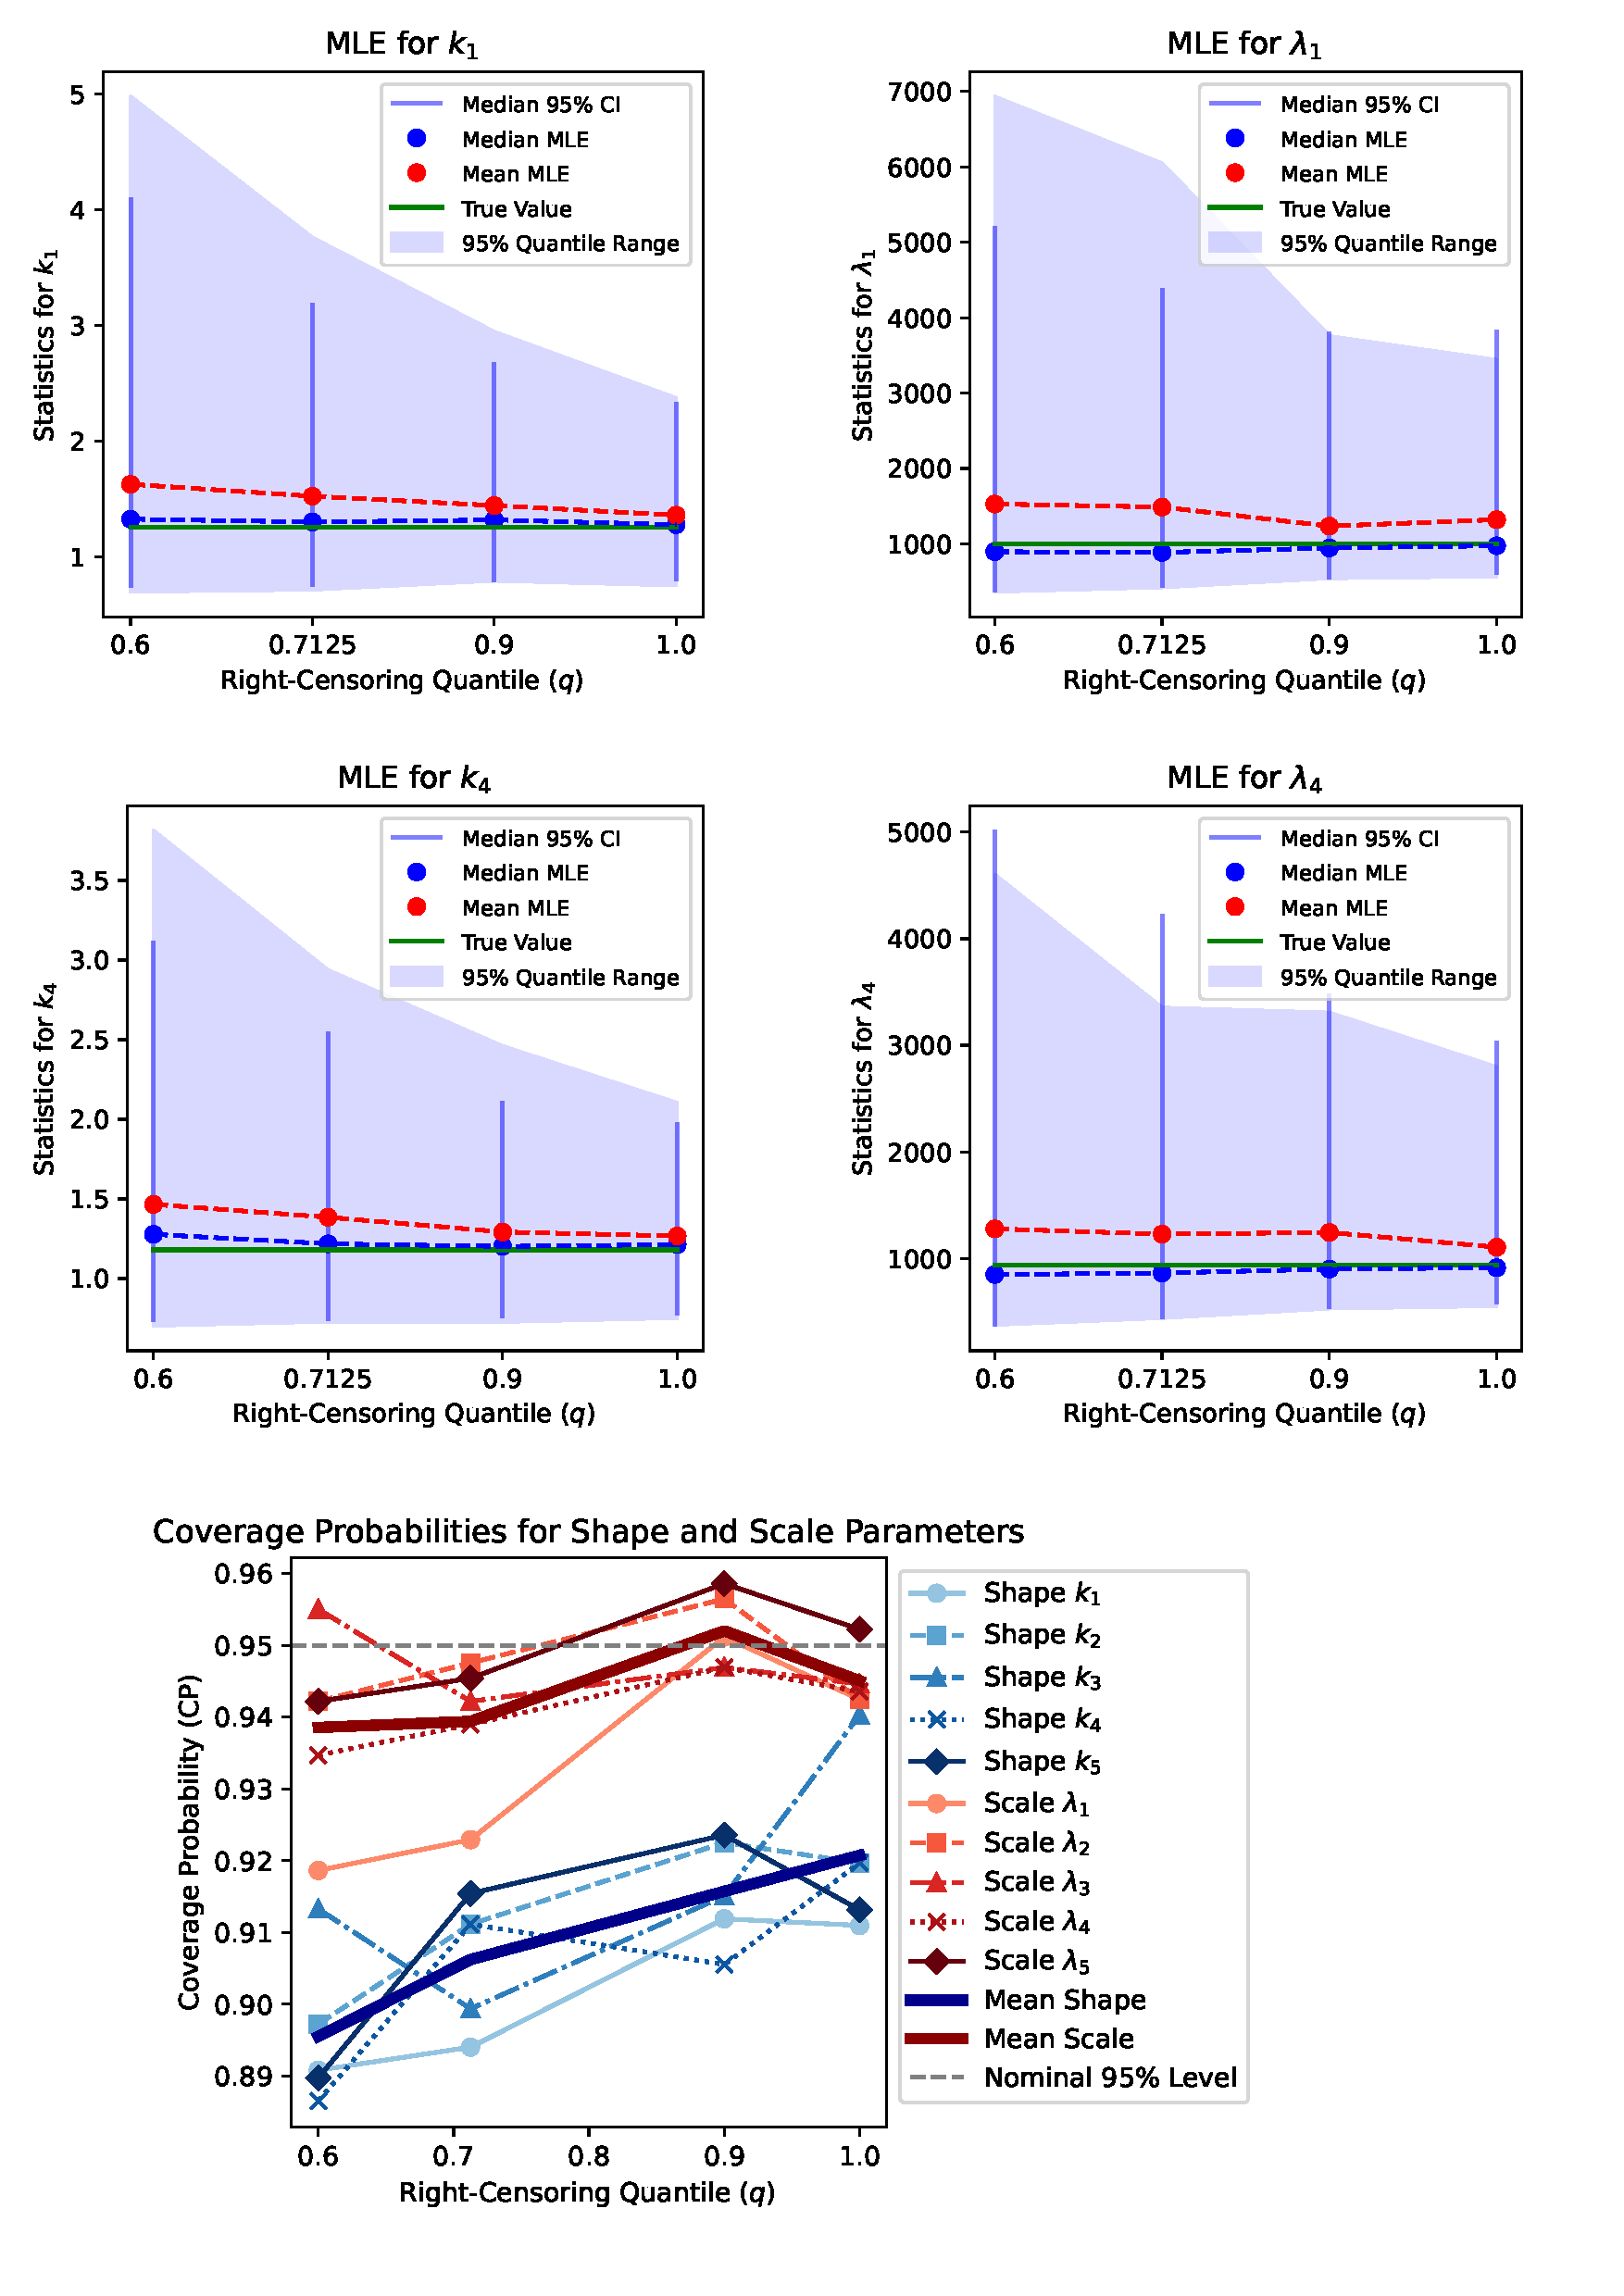
\includegraphics[width=1\linewidth]{image/5_system_tau_fig} 

}

\caption{Right-Censoring Quantile ($q$) vs MLE ($p = 0.215, n = 90$)}\label{fig:q-vs-stats}
\end{figure}

In Figure \ref{fig:q-vs-stats}, we show the effect of right-censoring on the
MLEs for the shape and scale parameters. The top four plots only show the effect
on the MLEs for the shape and scale parameters of components \(1\) and \(3\).
We chose these components because they are the most and least reliable
components, respectively, and so we expect them to be the most and least
sensitive to right-censoring. The bottom two plots show the coverage
probabilities for all parameters.

\hypertarget{background}{%
\subsubsection{Background}\label{background}}

When a right-censoring event occurs, in order to increase the likelihood of the data, the MLE
is nudged in a direction that increases the probability of a right-censoring event at time \(\tau\),
which is given by \(R_{T_i}(t;\boldsymbol{\theta})\), representing a source of bias in the estimate.

To increase \(R_{T_i}(\tau_q)\), we move in the direction (gradient) of these partial derivatives.
The partial derivatives of \(R_{T_i}(\tau_q)\) are given by
\begin{align*}
\frac{\partial R_{T_i}(\tau_q)}{\partial \lambda_j} &= R_{T_i}(\tau_q;\boldsymbol{\theta}) \left(\frac{\tau}{\lambda_j}\right)^{k_j} \frac{k_j}{\lambda_j},\\
\frac{\partial R_{T_i}(\tau_q)}{\partial k_j}       &= R_{T_i}(\tau_q;\boldsymbol{\theta}) \left(\frac{\tau}{\lambda_j}\right)^{k_j} \left(\log \lambda_j - \log \tau_q\right),
\end{align*}
for \(j = 1, \ldots, m\). We see that these partial derivatives are related to the score of a right-censored likelihood contribution in
Theorem \ref{thm:weibull-score}. Let us analyze the implications these
partial derivatives have on the MLE:

\begin{itemize}
\item
  \textbf{Effect of Increasing Right-Censoring Quantile}: As the right-censoring
  quantile \(q\) increases (\(\tau_q\) increases), \(R_{T_i}(\tau_q;\boldsymbol{\theta})\) decreases,
  reducing the impact of right-censoring on the MLE. This behavior is evident in
  Figure \ref{fig:q-vs-stats}.
\item
  \textbf{Positive Bias in Scale Parameters}: The partial derivatives with respect to
  the scale parameters are always positive. This means that right-censoring
  introduces a positive bias in the scale parameter estimates, making
  right-censoring events more likely. The extent of this bias is related
  to the amount of right-censoring (\(1-q\)), as seen in Figure \ref{fig:q-vs-stats}.
\item
  \textbf{Conditional Bias in Shape Parameters}: The partial derivative with respect
  to the shape parameter of the \(j\)\textsuperscript{th} component, \(k_j\), is
  non-negative if \(\lambda_j \geq \tau_q\) and otherwise negative. In our
  well-designed series system, the scale parameters are large compared to most of
  the right-censoring times \(\tau_q\), so the MLE nudges the shape parameter
  estimates in a positive direction to increase the probability \(R_{T_i}(\tau_q)\) of a
  right-censoring event at time \(\tau_q\). We see this in Figure
  \ref{fig:q-vs-stats}, where the shape parameter estimates are positively biased
  for most of the quantiles \(q\).
\end{itemize}

\hypertarget{key-observations}{%
\subsubsection{Key Observations}\label{key-observations}}

\hypertarget{coverage-probability-cp}{%
\subparagraph*{Coverage Probability (CP)}\label{coverage-probability-cp}}
\addcontentsline{toc}{subparagraph}{Coverage Probability (CP)}

The confidence intervals are generally correctly specified, obtaining coverages
above \(90\%\) for most of the parameters across the entire range of right-censoring
quantiles, and they are converging to the nominal \(95\%\) level as the
right-censoring quantile increases. This suggests that the bootstrapped CIs will
contain the true value of the parameters with the specified confidence level
with high probability. The CIs are neither too wide nor too narrow.

However, the scale parameters are better calibrated than the shape parameters.
The scale parameters are consistently around the nominal \(95\%\) level for all
right-censoring quantiles, but the shape parameters are consistently less
correctly specified, suggesting that the shape parameters are more difficult to
estimate than the scale parameters.

We also see that the coverage probabilities for \(k_1\) and \(\lambda_1\) generally
have worse coverage than the other parameters. This is likely due to the fact
that component 1 is the most reliable component, and so it is less likely to
fail before the right-censoring time \(\tau_q\). This means that the likelihood
contribution of component 1 is less informative than the other components.
Conversely, we see that \(k_3\) and \(\lambda_3\) generally have better coverage
than the other parameters. This is likely due to the fact that component 3 is
the least reliable component, and so it is more likely to fail before the
right-censoring time. This means that the likelihood contribution of component
3 is more informative than the other components in the presence of
right-censoring.

\hypertarget{dispersion-of-mles}{%
\subparagraph*{Dispersion of MLEs}\label{dispersion-of-mles}}
\addcontentsline{toc}{subparagraph}{Dispersion of MLEs}

The shaded regions representing the 95\% probability range of the MLEs get
narrower as the right-censoring quantile increases. This is an indicator of the
increased precision in the estimates as more data is available due to decreased
censoring.

We see that the dispersion of the MLEs for \(k_1\) and \(\lambda_1\) are much
larger than the dispersion of the MLEs for \(k_3\) and \(\lambda_3\). This is
consistent with the previous analysis for the coverage probabilities.

\hypertarget{median-aggregated-cis}{%
\subparagraph*{Median-Aggregated CIs}\label{median-aggregated-cis}}
\addcontentsline{toc}{subparagraph}{Median-Aggregated CIs}

The median CI (vertical blue bars) decreases in length as the right-censoring
quantile increases. This suggests that the bootstrapped CIs become more
consistent and centered around a tighter range as the right-censoring quantile
increases, while maintaining a good coverage probability. As right-censoring
events become less likely, the bootstrapped CIs gravitate closer to each other
and the true parameter values.

For small right-censoring quantiles, the CIs are quite large, which was
necessary to maintain good coverage. The estimator is sensitive to the data,
and so the bootstrapped CIs are wide to account for this sensitivity when the
sample contains insufficient information due to censoring. Again, we see
that the median-aggregated CIs for \(k_1\) and \(\lambda_1\) are much wider than
the median-aggregated CIs for \(k_3\) and \(\lambda_3\).

\hypertarget{bias-of-mles}{%
\subparagraph*{Bias of MLEs}\label{bias-of-mles}}
\addcontentsline{toc}{subparagraph}{Bias of MLEs}

The red dashed line indicating the mean of MLEs initially is quite biased
for the shape parameters, but quickly diminishes to negligible levels as the
right-censoring quantile increases. The bias for the shape parameters never
reach zero, but this is potentially due to masking.

The bias for the scale parameters is quite small and remains stable across
different right-censoring quantiles, suggesting that the scale MLEs are
reasonably unbiased. It could be the case that masking or other factors are
counteracting the bias due to right-censoring.

Again, we see that the bias for \(k_1\) and \(\lambda_1\) is much greater than the
bias for \(k_3\) and \(\lambda_3\), which is consistent with the previous analysis.

\hypertarget{convergence-rate}{%
\subparagraph*{Convergence Rate}\label{convergence-rate}}
\addcontentsline{toc}{subparagraph}{Convergence Rate}

The convergence rate increases as the right-censoring quantile \(q\)
increases. This is consistent with the expectation that more censoring
reduces the information in a sample, making the likelihood function less
informative and more difficult to identify the parameters that maximize it. We
see that the convergence rate is around \(95\%\) or greater for right-censoring
quantiles \(q \geq 0.7\), but drops below \(95\%\) for \(q < 0.7\).

\hypertarget{summary}{%
\subsubsection{Summary}\label{summary}}

In this scenario, we find that right-censoring significantly influences the MLEs
of shape and scale parameters. As the degree of right-censoring decreases, the
precision of these estimates improves, and the bias in the shape parameters
diminishes, although it never fully disappears, possibly due to masking effects.
Additionally, Bootstrapped (BCa) confidence intervals generally show good
coverage probabilities, particularly for scale parameters, and become more
focused as right-censoring decreases. As expected, the estimates for the most
reliable component are more sensitive to right-censoring than the least
reliable component. We also find that the convergence rate of the MLE decreases
as the degree of right-censoring increases, suggesting that the MLE is less
reliable in these cases.

These insights set the stage for the subsequent scenario on masking probability,
where we will explore how masking adds another layer of complexity to parameter
estimation and how these effects might be mitigated.

\hypertarget{p-vs-mttf}{%
\subsection{Scenario: Assessing the Impact of Masking Probability for Component Cause of Failure}\label{p-vs-mttf}}

In this scenario, we use the well-designed series system described in Table \ref{tab:series-sys}
and we use the following simulation scenario values:

\begin{itemize}
\tightlist
\item
  We vary the Bernoulli masking probability \(p\) from \(10\%\) to \(70\%\).\footnote{The probability that the component cause of failure is masked is the
    probability that at least one functional component will be in the
    candidate set, which is given by \(1 - (1 - p)^{m-1}\), where \(m\) denotes the number
    of components in the system and \(p\) is the Bernoulli masking probability. So, for
    \(m = 5\) and \(p\) ranges from \(10\%\) to \(70\%\), the probability that the component cause of
    failure is masked ranges from \(34.4\%\) to \(99.2\%\).}
\item
  We fix the right-censoring quantile \(q\) to \(82.5\%\), which means the probability
  of a right-censoring event is \(17.5\%\). This is less than the masking probability,
  making the masking probability the dominant source of uncertainty.
\item
  We fix the sample size to \(n\) to \(90\), which is small enough to show the impact of
  masking on the MLE, but large enough to obtain reasonable convergence rates.
\end{itemize}

In Figure \ref{fig:masking-prob-vs-stats}, we show the effect of the masking
probability \(p\) on the MLE for the shape and scale parameters. The top four
plots only show the effect on the MLE for the shape and scale parameters of
components \(1\) and \(3\), since the rest demonstrated similar results. The bottom
left plot shows the coverage probabilities for all parameters and the bottom
right plot shows the convergence rate of the MLE.

\begin{figure}

{\centering 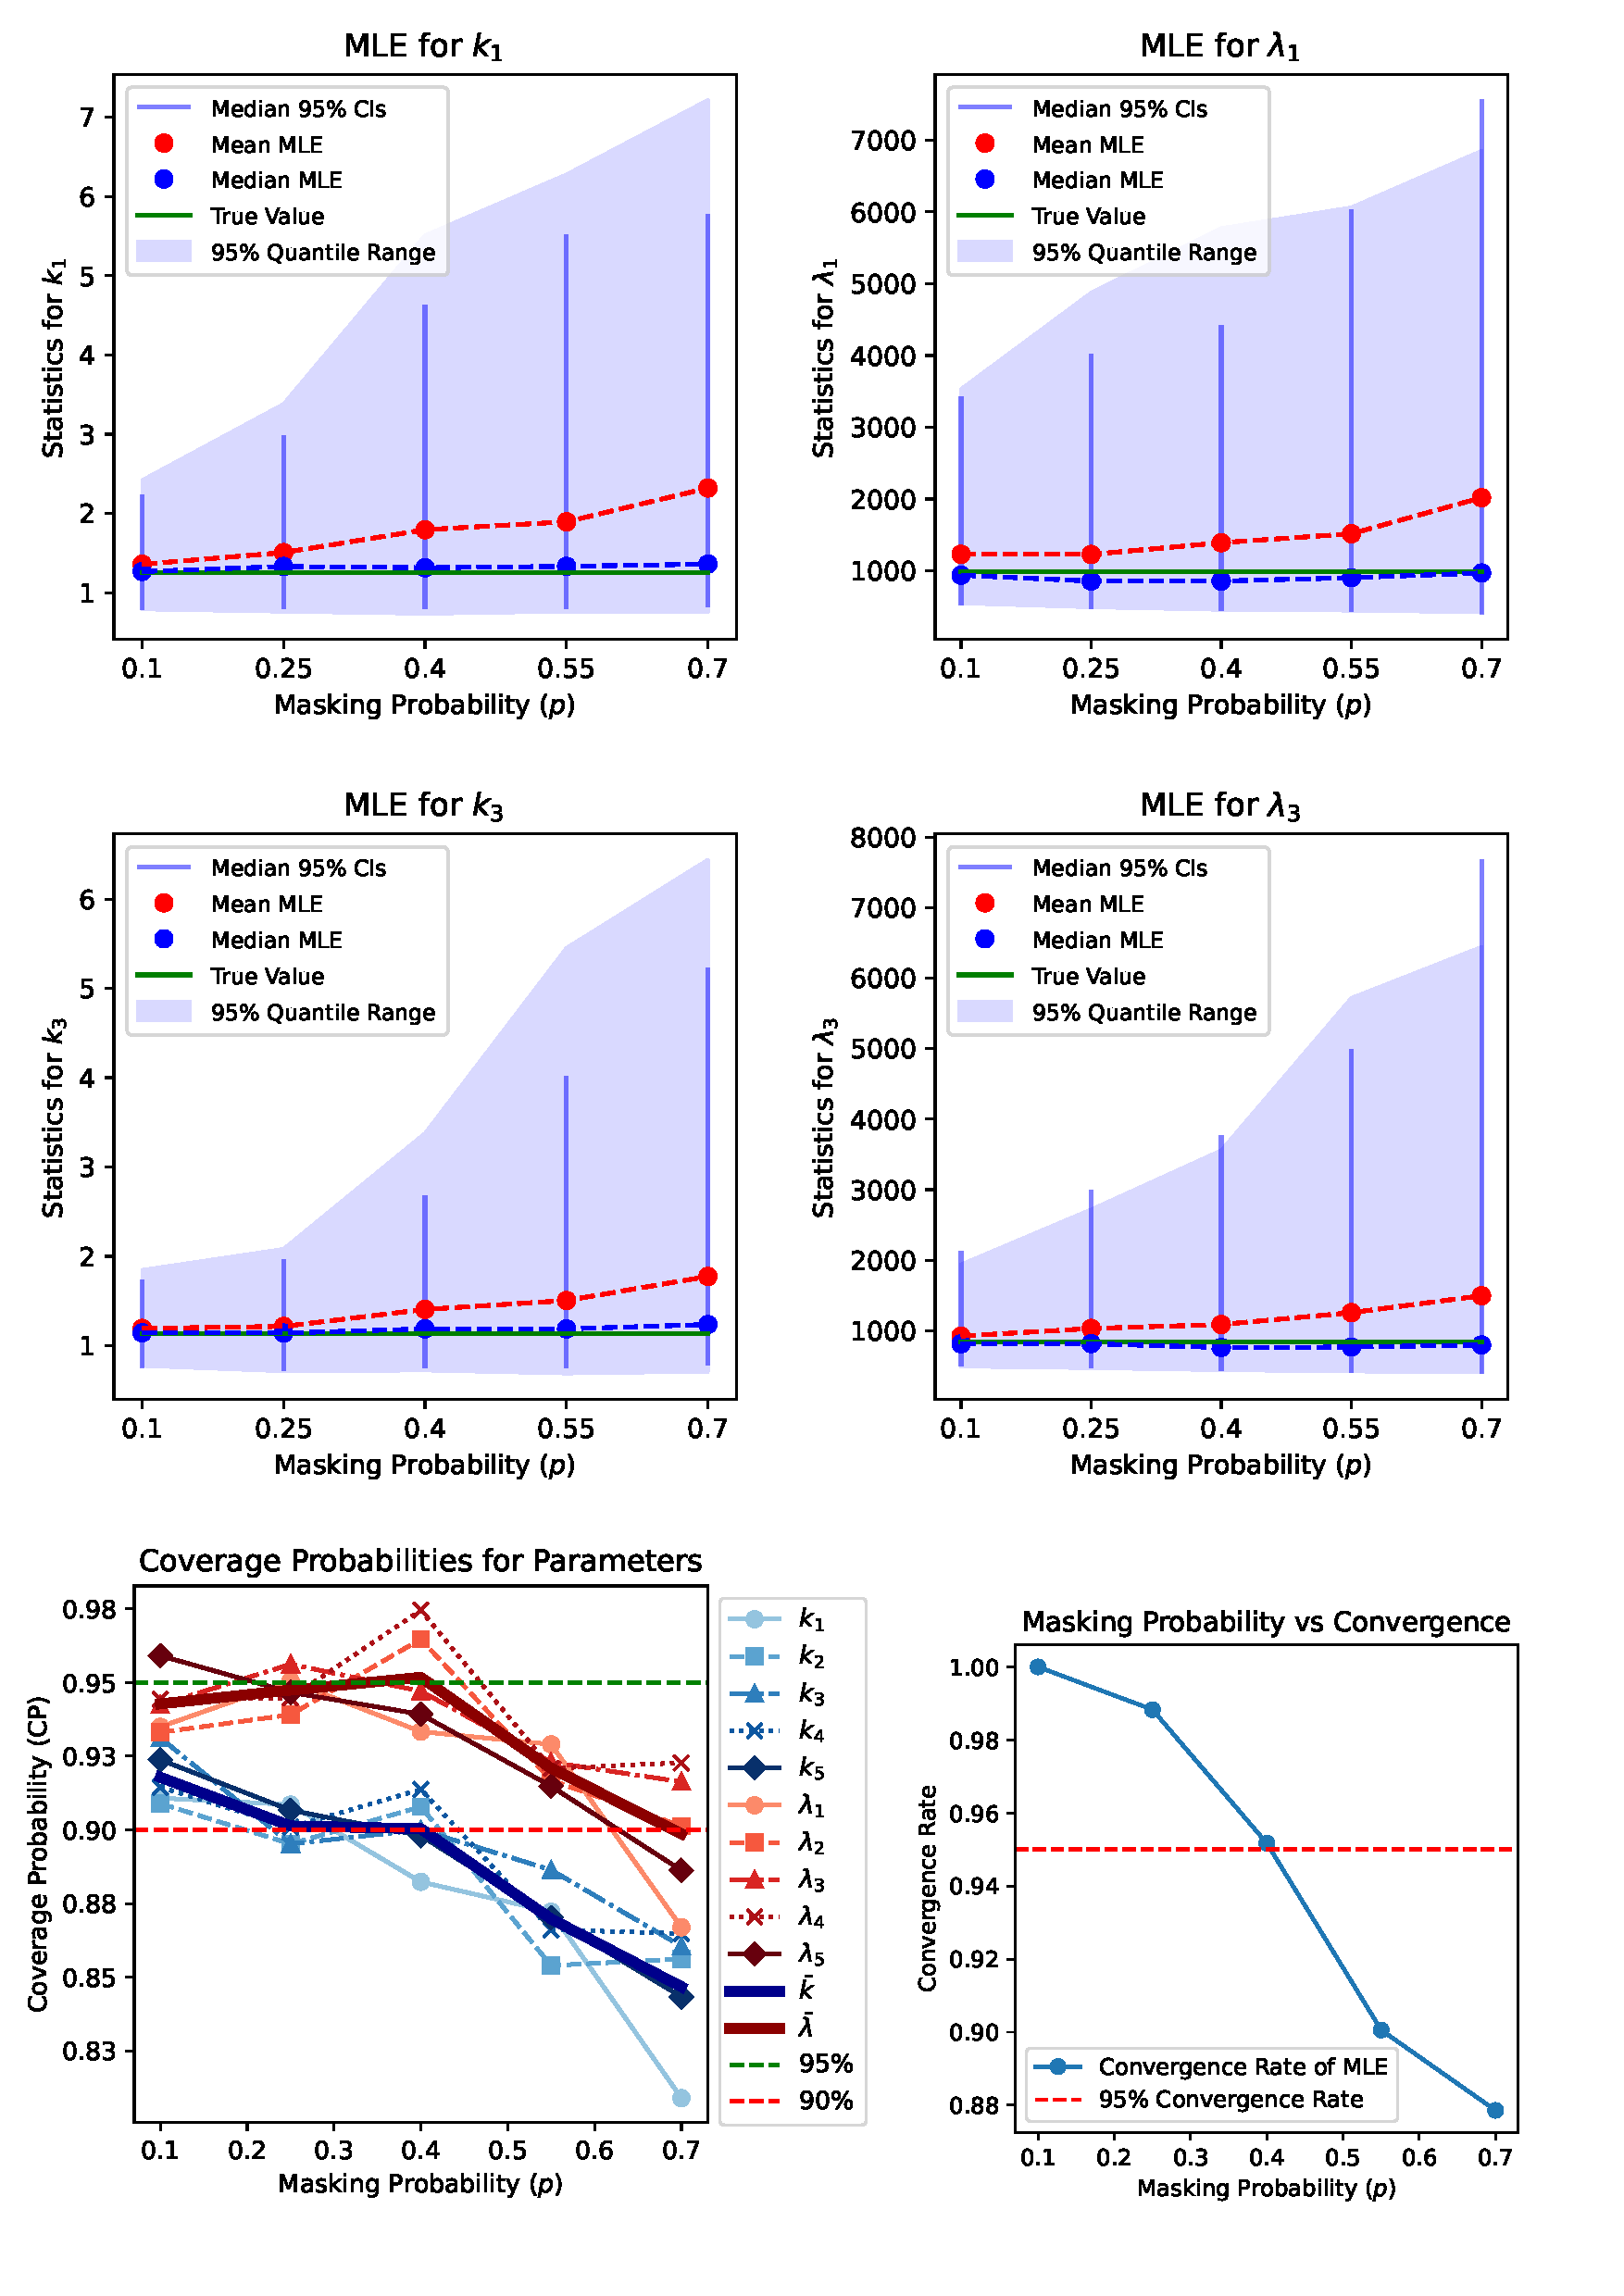
\includegraphics{image/5_system_prob_fig} 

}

\caption{Component Cause of Failure Masking ($p$) vs MLE ($q = 0.825, n = 90$)}\label{fig:masking-prob-vs-stats}
\end{figure}

\hypertarget{background-1}{%
\subsubsection{Background}\label{background-1}}

Masking introduces a layer of complexity that is different from right-censoring.
While right-censoring deals with the uncertainty in the timing of failure,
masking adds ambiguity in identifying which component actually failed. In the
Bernoulli masking model, the failed component is guaranteed to be in the
candidate set and each non-failed component is included with a probability \(p\).
This has the following implications on the MLE:

\begin{itemize}
\item
  \textbf{Ambiguity}: A higher \(p\) makes larger candidate sets more probable, making
  it less clear which parameter estimates should be adjusted to make the data
  more likely in the MLE. This is particularly problematic for components that are
  not the cause of failure, since the MLE will adjust their parameters to make
  them more likely to be the cause of failure, which is not necessarily correct.
\item
  \textbf{Bias}: In an ideal scenario, knowing which component failed would allow
  the MLE to make that component's failure more likely and a right-censoring
  effect would be applied to the non-failed components. However, a larger masking
  probability \(p\) introduces uncertainty, causing the MLE to adjust the estimates
  for the parameters of the non-failed components to be more likely to fail at the
  observed failure time while simultaneously applying a right-censoring effect to
  the other components, including the failed component. This introduces a bias
  similar to the bias introduced by right-censoring, and the greater the masking
  probability \(p\), the greater the bias.
\item
  \textbf{Precision}: As the masking probability \(p\) increases, the likelihood
  function becomes less informative, reducing the precision of the estimates.
\end{itemize}

\hypertarget{key-observations-1}{%
\subsubsection{Key Observations}\label{key-observations-1}}

\hypertarget{coverage-probability-cp-1}{%
\subparagraph*{Coverage Probability (CP)}\label{coverage-probability-cp-1}}
\addcontentsline{toc}{subparagraph}{Coverage Probability (CP)}

For the scale parameters, the \(95\%\) CI is correctly specified for Bernoulli
masking probabilities up to \(p = 0.7\), which is quite significant,
obtaining coverages over \(90\%\). For the shape parameters, the \(95\%\) CI is
correctly specified for masking probabilities only up to \(p = 0.4\), which is still
large. At \(p = 0.4\), the coverage probability is around \(90%
\), but continues to
drop after that point well below \(90\%\). This suggests that the shape parameters
are more difficult to estimate than the scale parameters, which is consistent
with the previous scenario where we varied the amount of right-censoring.

The BCa confidence intervals are correctly specified for most realistic masking
probabilities, constructing CIs that are neither too wide nor too narrow, but
when the masking is severe and the sample size is small, one should take the CIs
with a grain of salt.

\hypertarget{dispersion-of-mles-1}{%
\subparagraph*{Dispersion of MLEs}\label{dispersion-of-mles-1}}
\addcontentsline{toc}{subparagraph}{Dispersion of MLEs}

The shaded regions representing the \(95\%\) quantile of the MLEs become wider as
the masking probability increases. This is an indicator of the decreased
precision in the estimates when provided with more ambiguous data about the
component cause of failure.

\hypertarget{median-aggregated-cis-1}{%
\subparagraph*{Median-Aggregated CIs}\label{median-aggregated-cis-1}}
\addcontentsline{toc}{subparagraph}{Median-Aggregated CIs}

The median-aggregated CIs (vertical dark blue bars) show that the BCa CIs are
becoming more spread out as the masking probability increases. They are also
asymmetric, with the lower bound being more spread out than the upper-bound,
which is consistent with the behavior of the dispersion of the MLEs. The width
of the CIs consistently increase as the masking probability increases, which we
intuitively expected given the increased uncertainty about the component cause
of failure.

\hypertarget{bias-of-mles-1}{%
\subparagraph*{Bias of MLEs}\label{bias-of-mles-1}}
\addcontentsline{toc}{subparagraph}{Bias of MLEs}

The mean of the MLE (red dashed lines) demonstrates a steadily increasing
positive bias as the masking probability increases. This is consistent with the
expectation that the MLE will apply an increasing right-censoring effect to the
estimates as the masking probability increases.

\hypertarget{convergence-rate-1}{%
\subparagraph*{Convergence Rate}\label{convergence-rate-1}}
\addcontentsline{toc}{subparagraph}{Convergence Rate}

The convergence rate decreases as the Bernoulli masking probability \(p\)
increases. This is consistent with the expectation that a higher masking
probability decreases the information the sample contains about the
parameters. We see that the convergence rate remains above \(95\%\) for masking
probabilities up to \(p = 0.4\), but drops below \(95\%\) for \(p > 0.4\). This is
consistent with behavior of the CPs, which drop below \(90\%\) for \(p > 0.4\).

\hypertarget{summary-1}{%
\subsubsection{Summary}\label{summary-1}}

In this scenario, we examine the influence of masking probability \(p\) on the
MLE, keeping the sample size and right-censoring constant. As the masking
probability increases, the precision of the MLEs decreases,
and the coverage probability of the CIs begins to drop. However, even at fairly
significant Bernoulli masking probabilities, particularly for the scale
parameters, the CIs have good coverage. These observations highlight the
challenges of parameter estimation under varying degrees of masking and set the
stage for the subsequent scenario on sample size, which shows how increasing the
sample size can mitigate the effects of both right-censoring and masking.

\hypertarget{effect-samp-size}{%
\subsection{Scenario: Assessing the Impact of Sample Size}\label{effect-samp-size}}

In this scenario, we want to assess how the sample size can mitigate the affects of
right-censoring and masking previously discussed. We use the well-designed series
system described in Table \ref{tab:series-sys} and we use the following
simulation scenario values:

\begin{itemize}
\tightlist
\item
  We vary the sample size \(n\) from \(50\) (small sample size) to \(500\) (large sample size).
\item
  We fix the right-censoring quantile \(q\) to \(82.5\%\).
\item
  We fix the masking probability \(p\) to \(21.5\%\).
\end{itemize}

\begin{figure}

{\centering 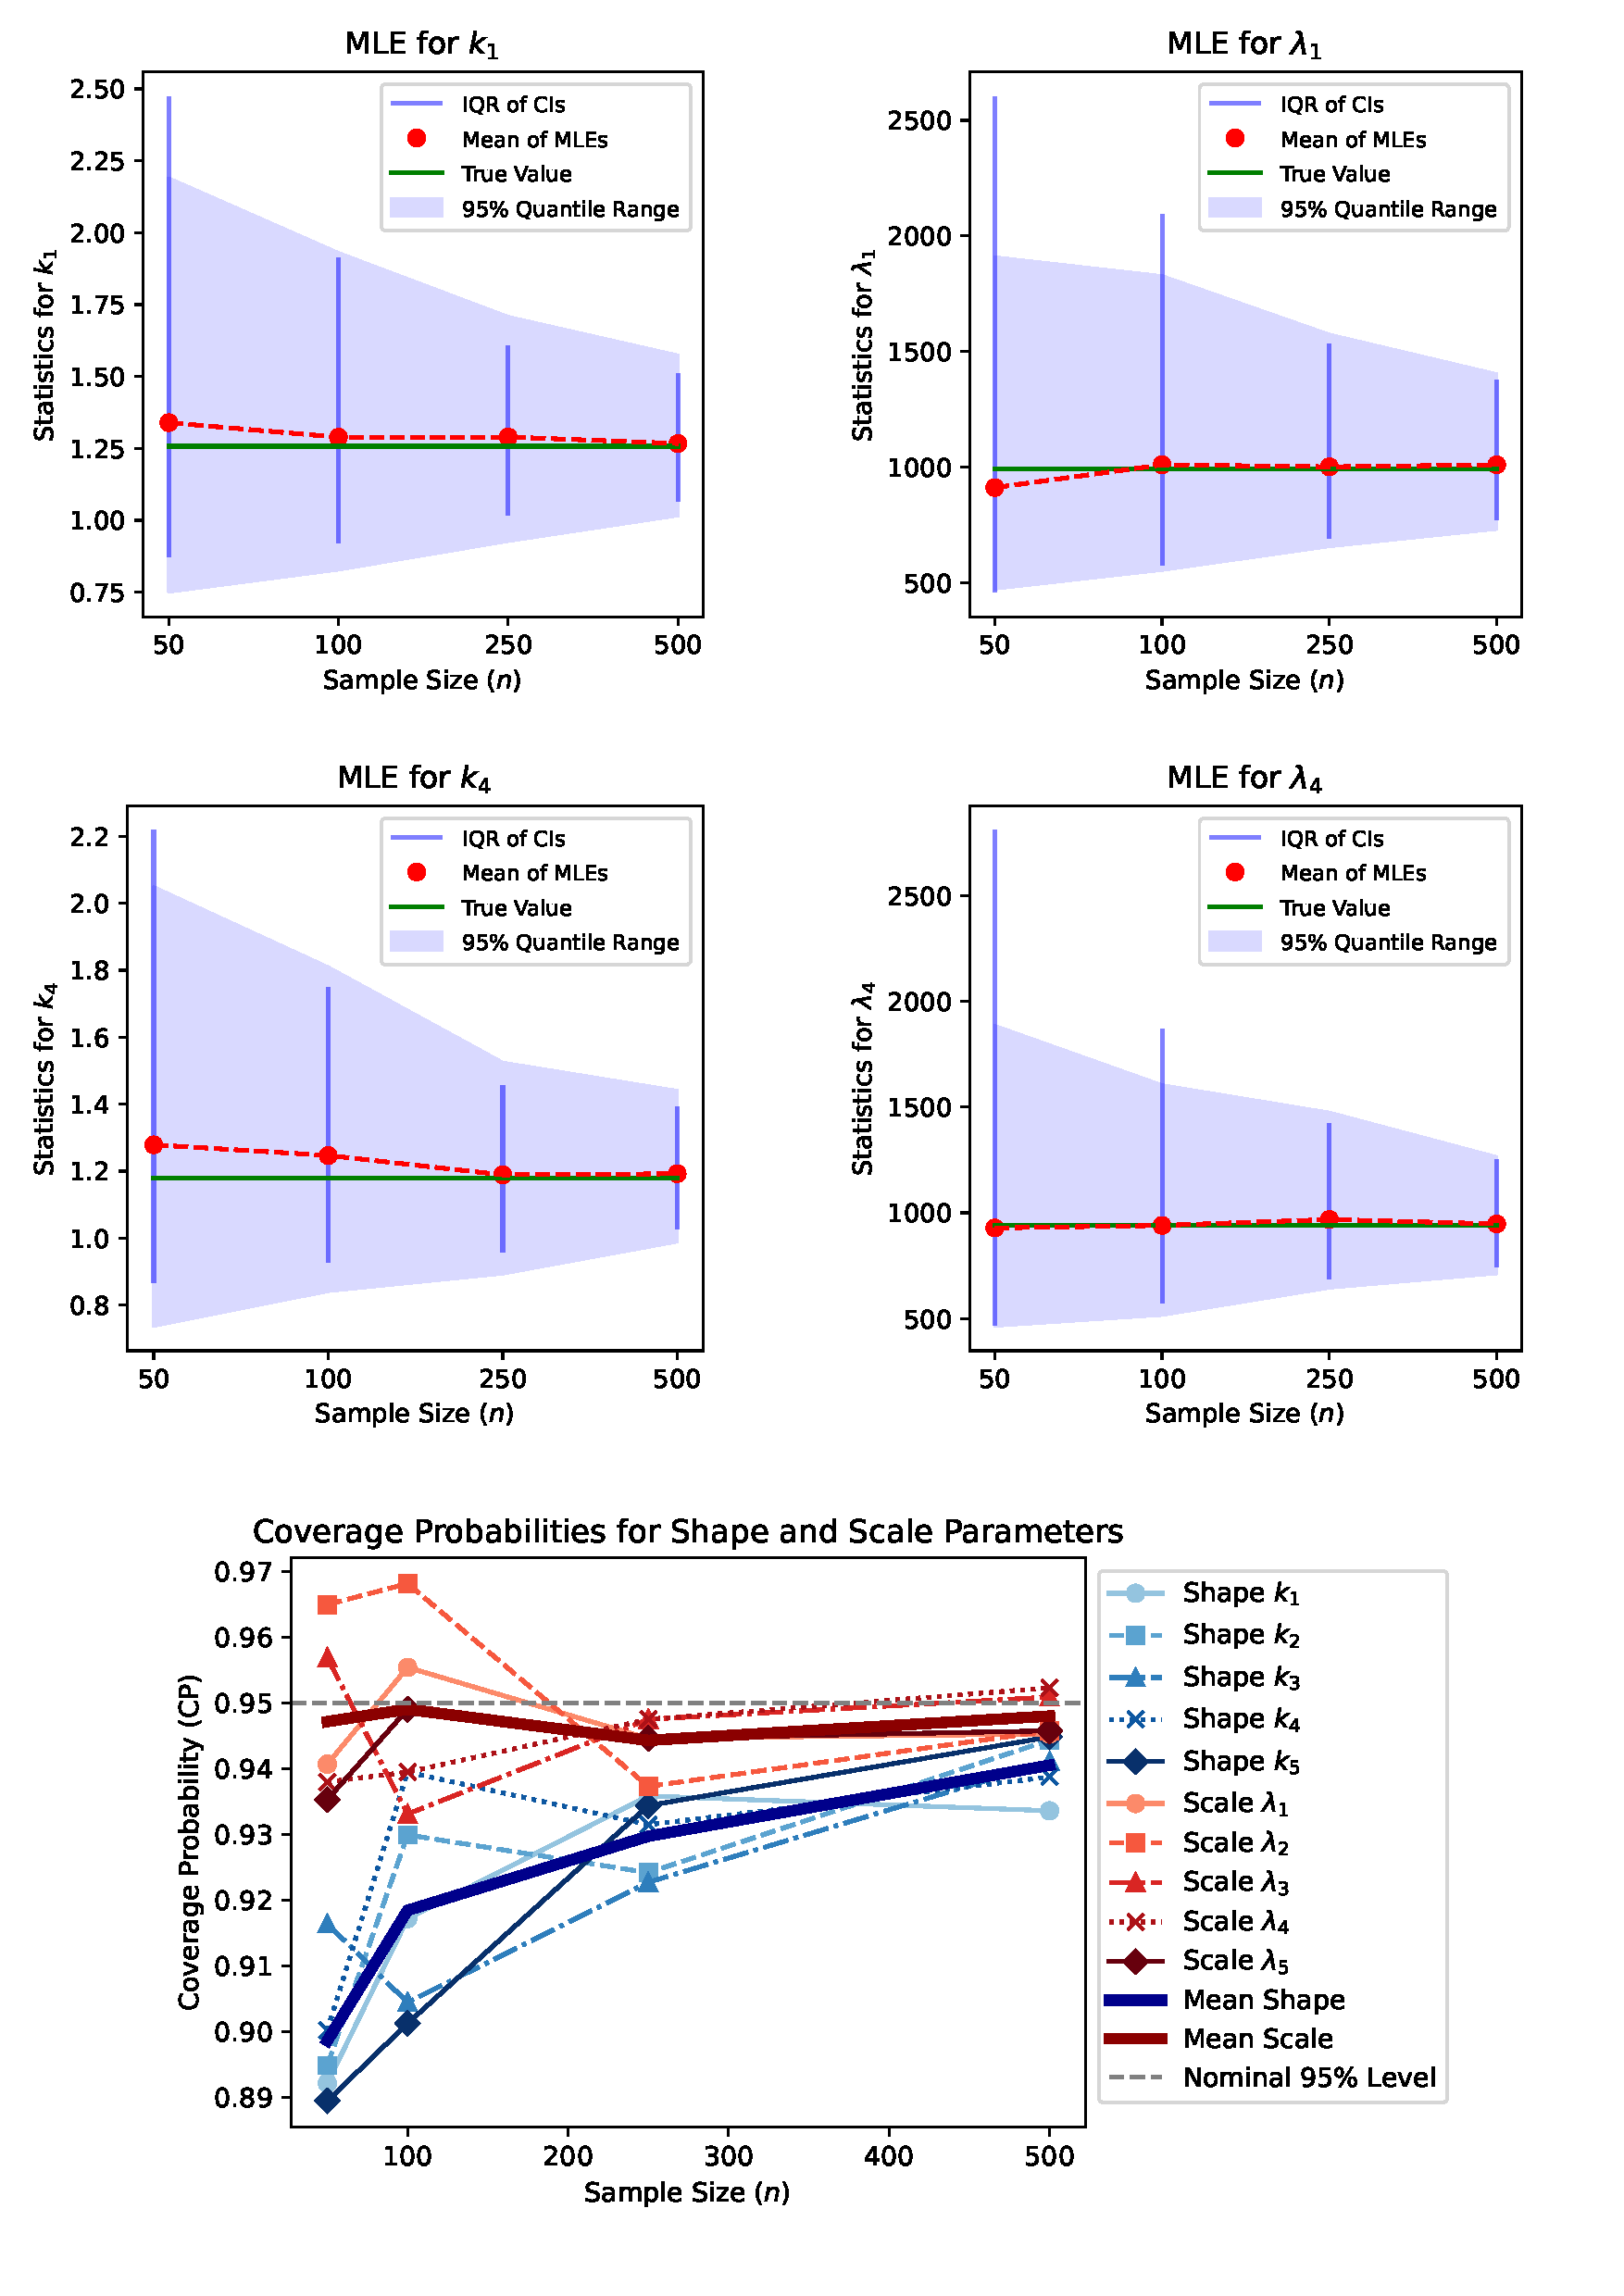
\includegraphics[width=1\linewidth]{image/5_system_samp_size_fig} 

}

\caption{Sample Size ($n$) vs MLEs ($p = 0.215, q = 0.825$)}\label{fig:samp-size-n-vs-stats}
\end{figure}

In Figure \ref{fig:samp-size-n-vs-stats}, we show the effect of the sample size
\(n\) on the MLEs for the shape and scale parameters. The top four plots only show
the effect on the MLEs for the shape and scale parameters of components \(1\) and
\(3\), component 1 being the most reliable component in the system and component 3
being the least reliable component. The bottom left plot shows the coverage
probabilities of the confidence intervals for all parameters and the bottom
right plot shows the convergence rate of the MLE.

\hypertarget{key-observations-2}{%
\subsubsection{Key Observations}\label{key-observations-2}}

\hypertarget{coverage-probability-cp-2}{%
\subparagraph*{Coverage Probability (CP)}\label{coverage-probability-cp-2}}
\addcontentsline{toc}{subparagraph}{Coverage Probability (CP)}

The confidence intervals are correctly specified, obtaining coverages
above \(90\%\) for most of the parameters across the entire sample size range,
and they are converging to the nominal \(95\%\) level as the sample size
increases. The BCa CIs contain the true value of the parameters with the
specified confidence level, and the CIs neither too wide nor too narrow.

However, as in the previous scenario where we varied the right-censoring
amount, the scale parameters have better coverage than the shape parameters.
The scale parameters are consistently around the nominal \(95\%\) level for all
sample sizes, but the shape parameters lag behind, suggesting that the shape
parameters are more difficult to estimate than the scale parameters.

\hypertarget{dispersion-of-mles-2}{%
\subparagraph*{Dispersion of MLEs}\label{dispersion-of-mles-2}}
\addcontentsline{toc}{subparagraph}{Dispersion of MLEs}

The shaded regions representing the \(95\%\) quantile range of the MLEs become
more narrow as the sample size increases. This is an indicator of the increased
precision in the estimates when provided with more data.

We also see that the dispersion of the MLEs for \(k_1\) and \(\lambda_1\) are much
larger than the dispersion of the MLEs for \(k_3\) and \(\lambda_3\). This is
consistent with the previous analysis in the right-censoring scenario.

\hypertarget{median-aggregated-cis-2}{%
\subparagraph*{Median-Aggregated CIs}\label{median-aggregated-cis-2}}
\addcontentsline{toc}{subparagraph}{Median-Aggregated CIs}

The median-aggregated CIs (vertical dark blue bars) show that the CIs are
becoming less spread out as the sample size increases, indicating that they are
becoming more consistent and centered around a tighter range while maintaining
good coverage probability. The end result is that we can construct more precise
and accurate CIs with larger samples and thus we can make more confident
inferences about the true parameter value.

The estimator is quite sensitive to the data, and so the CIs are wide to account
for this sensitivity when the sample size is small and not necessarily
representative of the true distribution.

We also observe that the upper bound of the CI is more spread out than the lower
bound. This is consistent with the behavior of the dispersion of the MLEs, which
have a positive bias. Thus, the CIs are accounting for this bias by being
more spread out in the direction of the bias.

\hypertarget{bias-of-mles-2}{%
\subparagraph*{Bias of MLEs}\label{bias-of-mles-2}}
\addcontentsline{toc}{subparagraph}{Bias of MLEs}

The mean of the MLE (red dashed lines) initially has a large positive
bias, but diminishes to negligible levels as the sample size increases. In the
previous right-censoring scenario, the bias never reached zero, but we see that
in this scenario, at around a sample size of \(250\), the estimator is essentially
unbiased, suggesting that there is enough information in the sample to overcome
the bias from the right-censoring (\(q = 0.825\)) and masking (\(p = 0.215\))
effects.

\hypertarget{convergence-rate-2}{%
\subparagraph*{Convergence Rate}\label{convergence-rate-2}}
\addcontentsline{toc}{subparagraph}{Convergence Rate}

The convergence rate increases as the sample size \(n\) increases. This is
consistent with the expectation that more data provides more information about
the parameters, making the likelihood function more informative and easier to
identify the parameters that maximize it. We see that the convergence rate is
\(95\%\) or greater for sample sizes \(n \geq 100\) given moderate right-censoring
and masking. Given how quickly the convergence rate increased, we anticipate
that even for extreme censoring and masking, the convergence rate would likely
rapidly increase to over \(95\%\) as the sample size increases. However, for
sample sizes \(n < 100\), at least for series systems with \(m = 5\) components with
Weibull lifetimes, the convergence rate is low. For small samples, any estimates
should be taken with a grain of salt.

\hypertarget{summary-2}{%
\subsubsection{Summary}\label{summary-2}}

In this scenario, we delve into the mitigating effects of sample size on the
challenges identified in previous scenarios concerning right-censoring and
masking. The precision and accuracy of the MLE rapidly improves with a bias
approaching zero. This is consistent with statistical theory and suggests that
increasing the sample size can mitigate the effects of right-censoring and
masking. The BCa CIs also narrow and become more reliable (with coverage
probabilities approaching the nominal \(95\%\) level) with larger samples,
reinforcing the role of sample size in achieving robust estimates.

\hypertarget{future-work}{%
\section{Future Work}\label{future-work}}

This paper developed maximum likelihood techniques and simulation studies to
estimate component reliability from masked failure data in series systems. The
key results were:

\begin{itemize}
\tightlist
\item
  The likelihood model enabled rigorous inference from masked data via
  right-censoring and candidate sets.
\item
  Despite masking and censoring, the MLE demonstrated accurate and robust
  performance in simulation studies.
\item
  BCa confidence intervals had good coverage probability even for small samples.
\item
  Estimation of shape parameters was more challenging than scale parameters.
\end{itemize}

Building on these findings, next we consider promising areas for future work.

\hypertarget{relaxing-masking-conditions}{%
\paragraph*{Relaxing Masking Conditions}\label{relaxing-masking-conditions}}
\addcontentsline{toc}{paragraph}{Relaxing Masking Conditions}

To further generalize the likelihood model, we can relax conditions
\ref{cond:c-contains-k}, \ref{cond:equal-prob-failure-cause}, and
\ref{cond:masked-indept-theta} on the masking model. We could perform
a sensitivity analysis to violations of these conditions, which would provide
insights into the robustness of the likelihood model, or we could develop
alternative likelihood models that are less stringent.

\hypertarget{deviations-from-well-designed-series-systems}{%
\paragraph*{Deviations from Well-Designed Series Systems}\label{deviations-from-well-designed-series-systems}}
\addcontentsline{toc}{paragraph}{Deviations from Well-Designed Series Systems}

Assess the sensitivity of the estimator to deviations from well-designed
series systems, in which there are no components that are significantly more
likely to fail than others. We could vary the probabilities of component failure
(while keeping the system reliability constant) to assess how the estimator
behaves when the system deviates from the well-designed system criteria. We did
some preliminary investigation of this, and we found that the estimator was
quite sensitive to deviations in system design.

\hypertarget{homogenous-shape-parameter}{%
\paragraph*{Homogenous Shape Parameter}\label{homogenous-shape-parameter}}
\addcontentsline{toc}{paragraph}{Homogenous Shape Parameter}

Assess the trade-off between using the homogenous shape parameter model and the
full model. The homogenous shape parameter model assumes that the shape
parameters are equal, which is a simplification of the full model. We could
assess the sensitivity of the estimator to deviations in the homogenous shape
parameter assumption. By the bias-variance trade-off, we expect that
the homogenous shape parameter model will have less variance but more bias than
the full model.\footnote{The bias-variance trade-off is a fundamental trade-off in statistics
  that states that as the bias of an estimator decreases, its variance
  increases, and vice versa. An estimator with more variance is
  more sensitive to the data, while an estimator with more bias is less
  sensitive to the data. If the assumption of homogeneity is reasonable, then
  the bias can be quite small while the variance is also small, potentially
  making the homogenous shape parameter model a good choice in such cases.} We did some preliminary investigation of this, and we
found that the homogenous shape parameter model worked quite well for
moderate masking and censoring when the true system was a reasonably
well-designed series system, and only had more bias than the full model when
the sample size was extremely large.

\hypertarget{semi-parametric-bootstrap}{%
\paragraph*{Semi-Parametric Bootstrap}\label{semi-parametric-bootstrap}}
\addcontentsline{toc}{paragraph}{Semi-Parametric Bootstrap}

We used the non-parametric bootstrap to construct confidence intervals, but we
could also investigate the semi-parametric bootstrap. In the semi-parametric
bootstrap, instead of resampling from the original data, we sample component
lifetimes from the parametric distribution fitted to the original data and
sample candidate sets from the conditional empirical distribution of the
candidate sets in the original data. This is a compromise between the
non-parametric bootstrap and the fully parametric bootstrap.\footnote{The fully parametric bootstrap is not appropriate for our likelihood
  model because we do not assume a parametric form for the distribution of the
  candidate sets.}

\hypertarget{regularization-methods}{%
\paragraph*{Regularization Methods}\label{regularization-methods}}
\addcontentsline{toc}{paragraph}{Regularization Methods}

Investigate regularization methods like data augmentation and penalized
likelihood to improve parameter estimates, in particular shape parameter
estimates.

\hypertarget{extending-the-likelihood-model-with-predictors}{%
\paragraph*{Extending the Likelihood Model with Predictors}\label{extending-the-likelihood-model-with-predictors}}
\addcontentsline{toc}{paragraph}{Extending the Likelihood Model with Predictors}

Our research is based on a general likelihood model. A straightforward extension
is to integrate predictors, allowing each observation's hazard function to be
influenced by specific variables, such as in the Cox proportional hazards model
\citep{cox1972regression}, but any function that satisfies the fundamental
mathematical principles of a hazard function could be used. This would allow
the likelihood model to be more flexible and adaptable to a wider range of
applications.

\hypertarget{bootstrapped-prediction-intervals}{%
\paragraph*{Bootstrapped Prediction Intervals}\label{bootstrapped-prediction-intervals}}
\addcontentsline{toc}{paragraph}{Bootstrapped Prediction Intervals}

In this paper, we applied the bootstrap method to construct confidence
intervals for the parameter \(\boldsymbol{\theta}\), which generated correctly specified
confidence intervals in our simulation study. We could do a similar analysis for
other statistics, in particular prediction intervals, which are useful for
predicting the reliability of a system or a component at a future time.

The current results provide a solid foundation for extensions like these that
can further refine the methods and expand their applicability. By leveraging the
rigorous likelihood framework and simulation techniques validated in this study,
future work can continue advancing the capability for statistical learning from
masked reliability data.

\hypertarget{conclusion}{%
\section{Conclusion}\label{conclusion}}

This work presented maximum likelihood techniques to estimate component
reliability from masked failure data in series systems. The methods demonstrated
accurate and robust performance despite significant challenges introduced by
masking and right-censoring.

Simulation studies revealed that for our well-designed series system with
Weibull component lifetimes, right-censoring and masking positively biased the
estimates and the more reliable components were more sensitive to these effects.
Additionally, the shape parameters were more difficult to estimate than the
scale parameters. However, with sufficiently large sample sizes, these
difficulties were overcome, suggesting enough information existed in the data to
mitigate censoring and masking effects.

Despite the challenges, the bootstrapped bias-corrected and accelerated
confidence intervals were generally correctly specified with good overall
coverage probabilities, even for relatively small sample sizes. This good
empirical coverage demonstrates the reliability of these intervals for
statistical inference, striking a balance between precision and robustness. The
modeling framework offers a statistically rigorous method for estimating latent
component properties based on limited observational data concerning system
reliability. The simulation studies validate these techniques and provide
practical insights into their efficacy under diverse real-world scenarios. This
enhances our capacity for statistical learning from obscured system failure
data.

\hypertarget{appendices}{%
\section*{Appendices}\label{appendices}}
\addcontentsline{toc}{section}{Appendices}

\hypertarget{appendix-appendix}{%
\appendix}


\hypertarget{series-system-with-weibull-component-lifetimes}{%
\section{Series System with Weibull Component Lifetimes}\label{series-system-with-weibull-component-lifetimes}}

These functions are implemented in the R library \texttt{wei.series.md.c1.c2.c3}, which
is available on GitHub at
\href{https://github.com/queelius/wei.series.md.c1.c2.c3}{\texttt{github.com/queelius/wei.series.md.c1.c2.c3}}
\citep{towell2023weibull}.
They are for series systems with Weibull component lifetimes with masked data
described in Section \ref{like-model}. For clarity and brevity, we
removed some of the functionality and safeguards in the actual code, but we
provide the full code in the R package.

\hypertarget{app-weibull-loglik-r}{%
\subsection{Log-likelihood Function}\label{app-weibull-loglik-r}}

The log-likelihood function is the sum of the log-likelihood contributions for
each system. For our series system with Weibull component lifetimes, we
analytically derived the log-likelihood function in Theorem
\ref{thm:weibull-likelihood-contribution} and implemented it in the
\texttt{loglik\_wei\_series\_md\_c1\_c2\_c3} R function below.

\begin{Shaded}
\begin{Highlighting}[]
\CommentTok{\#\textquotesingle{} Generates a log{-}likelihood function for a series system with Weibull}
\CommentTok{\#\textquotesingle{} component lifetimes for masked data.}
\CommentTok{\#\textquotesingle{}}
\CommentTok{\#\textquotesingle{} @param df masked data frame}
\CommentTok{\#\textquotesingle{} @param theta parameter vector}
\CommentTok{\#\textquotesingle{} @returns log{-}likelihood function}
\NormalTok{loglik\_wei\_series\_md\_c1\_c2\_c3 \textless{}{-}}\StringTok{ }\ControlFlowTok{function}\NormalTok{(df, theta) \{}
\NormalTok{  n \textless{}{-}}\StringTok{ }\KeywordTok{nrow}\NormalTok{(df)}
\NormalTok{  C \textless{}{-}}\StringTok{ }\KeywordTok{md\_decode\_matrix}\NormalTok{(df, }\StringTok{"x"}\NormalTok{)}
\NormalTok{  m \textless{}{-}}\StringTok{ }\KeywordTok{ncol}\NormalTok{(C)}
\NormalTok{  delta \textless{}{-}}\StringTok{ }\NormalTok{df[[}\StringTok{"delta"}\NormalTok{]]}
\NormalTok{  shapes \textless{}{-}}\StringTok{ }\NormalTok{theta[}\KeywordTok{seq}\NormalTok{(}\DecValTok{1}\NormalTok{, }\KeywordTok{length}\NormalTok{(theta), }\DecValTok{2}\NormalTok{)]}
\NormalTok{  scales \textless{}{-}}\StringTok{ }\NormalTok{theta[}\KeywordTok{seq}\NormalTok{(}\DecValTok{2}\NormalTok{, }\KeywordTok{length}\NormalTok{(theta), }\DecValTok{2}\NormalTok{)]}
\NormalTok{  t \textless{}{-}}\StringTok{ }\NormalTok{df[[lifetime]]}
\NormalTok{  s \textless{}{-}}\StringTok{ }\DecValTok{0}
  \ControlFlowTok{for}\NormalTok{ (i }\ControlFlowTok{in} \DecValTok{1}\OperatorTok{:}\NormalTok{n) \{}
\NormalTok{    s \textless{}{-}}\StringTok{ }\NormalTok{s }\OperatorTok{{-}}\StringTok{ }\KeywordTok{sum}\NormalTok{((t[i] }\OperatorTok{/}\StringTok{ }\NormalTok{scales)}\OperatorTok{\^{}}\NormalTok{shapes)}
    \ControlFlowTok{if}\NormalTok{ (delta[i]) \{}
\NormalTok{      s \textless{}{-}}\StringTok{ }\NormalTok{s }\OperatorTok{+}\StringTok{ }\KeywordTok{log}\NormalTok{(}\KeywordTok{sum}\NormalTok{(shapes[C[i, ]] }\OperatorTok{/}\StringTok{ }\NormalTok{scales[C[i, ]] }\OperatorTok{*}
\StringTok{        }\NormalTok{(t[i] }\OperatorTok{/}\StringTok{ }\NormalTok{scales[C[i, ]])}\OperatorTok{\^{}}\NormalTok{(shapes[C[i, ]] }\OperatorTok{{-}}\StringTok{ }\DecValTok{1}\NormalTok{)))}
\NormalTok{    \}}
\NormalTok{  \}}
  \KeywordTok{return}\NormalTok{(s)}
\NormalTok{\}}
\end{Highlighting}
\end{Shaded}

\hypertarget{app-score-fn-r}{%
\subsection{Score Function}\label{app-score-fn-r}}

The score function is the gradient of the log-likelihood function. For our
series system with Weibull component lifetimes, we analytically derived the
score function in Theorem \ref{thm:weibull-score} and implemented it in
the \texttt{score\_wei\_series\_md\_c1\_c2\_c3} R function below.

\begin{Shaded}
\begin{Highlighting}[]
\CommentTok{\#\textquotesingle{} Computes the score function for a series system with Weibull component}
\CommentTok{\#\textquotesingle{} lifetimes for masked data.}
\CommentTok{\#\textquotesingle{}}
\CommentTok{\#\textquotesingle{} @param df masked data frame}
\CommentTok{\#\textquotesingle{} @param theta parameter vector}
\CommentTok{\#\textquotesingle{} @returns score function}
\NormalTok{score\_wei\_series\_md\_c1\_c2\_c3 \textless{}{-}}\StringTok{ }\ControlFlowTok{function}\NormalTok{(df, theta) \{}
\NormalTok{  n \textless{}{-}}\StringTok{ }\KeywordTok{nrow}\NormalTok{(df)}
\NormalTok{  C \textless{}{-}}\StringTok{ }\KeywordTok{md\_decode\_matrix}\NormalTok{(df, }\StringTok{"x"}\NormalTok{)}
\NormalTok{  m \textless{}{-}}\StringTok{ }\KeywordTok{ncol}\NormalTok{(C)}
\NormalTok{  delta \textless{}{-}}\StringTok{ }\NormalTok{df[[}\StringTok{"delta"}\NormalTok{]]}
\NormalTok{  t \textless{}{-}}\StringTok{ }\NormalTok{df[[lifetime]]}
\NormalTok{  shapes \textless{}{-}}\StringTok{ }\NormalTok{theta[}\KeywordTok{seq}\NormalTok{(}\DecValTok{1}\NormalTok{, }\KeywordTok{length}\NormalTok{(theta), }\DecValTok{2}\NormalTok{)]}
\NormalTok{  scales \textless{}{-}}\StringTok{ }\NormalTok{theta[}\KeywordTok{seq}\NormalTok{(}\DecValTok{2}\NormalTok{, }\KeywordTok{length}\NormalTok{(theta), }\DecValTok{2}\NormalTok{)]}
\NormalTok{  shapes.scr \textless{}{-}}\StringTok{ }\NormalTok{scales.scr \textless{}{-}}\StringTok{ }\KeywordTok{rep}\NormalTok{(}\DecValTok{0}\NormalTok{, m)}

  \ControlFlowTok{for}\NormalTok{ (i }\ControlFlowTok{in} \DecValTok{1}\OperatorTok{:}\NormalTok{n) \{}
\NormalTok{    shapes.rt \textless{}{-}}\StringTok{ }\OperatorTok{{-}}\NormalTok{(t[i] }\OperatorTok{/}\StringTok{ }\NormalTok{scales)}\OperatorTok{\^{}}\NormalTok{shapes }\OperatorTok{*}\StringTok{ }\KeywordTok{log}\NormalTok{(t[i] }\OperatorTok{/}\StringTok{ }\NormalTok{scales)}
\NormalTok{    scales.rt \textless{}{-}}\StringTok{ }\NormalTok{(shapes }\OperatorTok{/}\StringTok{ }\NormalTok{scales) }\OperatorTok{*}\StringTok{ }\NormalTok{(t[i] }\OperatorTok{/}\StringTok{ }\NormalTok{scales)}\OperatorTok{\^{}}\NormalTok{shapes}
\NormalTok{    shapes.trm \textless{}{-}}\StringTok{ }\NormalTok{scales.trm \textless{}{-}}\StringTok{ }\KeywordTok{rep}\NormalTok{(}\DecValTok{0}\NormalTok{, m)}

    \ControlFlowTok{if}\NormalTok{ (delta[i]) \{}
\NormalTok{      c \textless{}{-}}\StringTok{ }\NormalTok{C[i, ]}
\NormalTok{      denom \textless{}{-}}\StringTok{ }\KeywordTok{sum}\NormalTok{(shapes[c] }\OperatorTok{/}\StringTok{ }\NormalTok{scales[c] }\OperatorTok{*}
\StringTok{        }\NormalTok{(t[i] }\OperatorTok{/}\StringTok{ }\NormalTok{scales[c])}\OperatorTok{\^{}}\NormalTok{(shapes[c] }\OperatorTok{{-}}\StringTok{ }\DecValTok{1}\NormalTok{))}

\NormalTok{      shapes.num \textless{}{-}}\StringTok{ }\NormalTok{(t[i] }\OperatorTok{/}\StringTok{ }\NormalTok{scales[c])}\OperatorTok{\^{}}\NormalTok{shapes[c] }\OperatorTok{/}\StringTok{ }\NormalTok{t[i] }\OperatorTok{*}
\StringTok{        }\NormalTok{(}\DecValTok{1} \OperatorTok{+}\StringTok{ }\NormalTok{shapes[c] }\OperatorTok{*}\StringTok{ }\KeywordTok{log}\NormalTok{(t[i] }\OperatorTok{/}\StringTok{ }\NormalTok{scales[c]))}
\NormalTok{      shapes.trm[c] \textless{}{-}}\StringTok{ }\NormalTok{shapes.num }\OperatorTok{/}\StringTok{ }\NormalTok{denom}

\NormalTok{      scales.num \textless{}{-}}\StringTok{ }\NormalTok{(shapes[c] }\OperatorTok{/}\StringTok{ }\NormalTok{scales[c])}\OperatorTok{\^{}}\DecValTok{2} \OperatorTok{*}
\StringTok{        }\NormalTok{(t[i] }\OperatorTok{/}\StringTok{ }\NormalTok{scales[c])}\OperatorTok{\^{}}\NormalTok{(shapes[c] }\OperatorTok{{-}}\StringTok{ }\DecValTok{1}\NormalTok{)}
\NormalTok{      scales.trm[c] \textless{}{-}}\StringTok{ }\NormalTok{scales.num }\OperatorTok{/}\StringTok{ }\NormalTok{denom}
\NormalTok{    \}}

\NormalTok{    shapes.scr \textless{}{-}}\StringTok{ }\NormalTok{shapes.scr }\OperatorTok{+}\StringTok{ }\NormalTok{shapes.rt }\OperatorTok{+}\StringTok{ }\NormalTok{shapes.trm}
\NormalTok{    scales.scr \textless{}{-}}\StringTok{ }\NormalTok{scales.scr }\OperatorTok{+}\StringTok{ }\NormalTok{scales.rt }\OperatorTok{{-}}\StringTok{ }\NormalTok{scales.trm}
\NormalTok{  \}}

\NormalTok{  scr \textless{}{-}}\StringTok{ }\KeywordTok{rep}\NormalTok{(}\DecValTok{0}\NormalTok{, }\KeywordTok{length}\NormalTok{(theta))}
\NormalTok{  scr[}\KeywordTok{seq}\NormalTok{(}\DecValTok{1}\NormalTok{, }\KeywordTok{length}\NormalTok{(theta), }\DecValTok{2}\NormalTok{)] \textless{}{-}}\StringTok{ }\NormalTok{shapes.scr}
\NormalTok{  scr[}\KeywordTok{seq}\NormalTok{(}\DecValTok{2}\NormalTok{, }\KeywordTok{length}\NormalTok{(theta), }\DecValTok{2}\NormalTok{)] \textless{}{-}}\StringTok{ }\NormalTok{scales.scr}
  \KeywordTok{return}\NormalTok{(scr)}
\NormalTok{\}}
\end{Highlighting}
\end{Shaded}

\hypertarget{app-series-quantile}{%
\subsection{Quantile Function}\label{app-series-quantile}}

For our series system with Weibull component lifetimes, the quantile function is
the inverse of the cdf \(F_{T_i}\). By definition, the quantile \(p\) for the strictly
monotonically increasing cdf \(F_{T_i}\) is the value \(t\) that satisfies
\(F_{T_i}(t;\boldsymbol{\theta}) - p = 0\), and so we solve for \(t\) using Newton's method,
in which the \(k\)\textsuperscript{th} iteration is given by
\[
t^{(k+1)} = t^{(k)} - \frac{F_{T_i}(t^{(k)};\boldsymbol{\theta}) - p}{f_{T_i}(t^{(k)};\boldsymbol{\theta})}.
\]
We have derived a slightly more efficient method in the \texttt{qwei\_series} R function
below.

\begin{Shaded}
\begin{Highlighting}[]
\CommentTok{\#\textquotesingle{} Quantile function for a series system with Weibull component lifetimes.}
\CommentTok{\#\textquotesingle{}}
\CommentTok{\#\textquotesingle{} @param p quantile}
\CommentTok{\#\textquotesingle{} @param shapes shape parameters}
\CommentTok{\#\textquotesingle{} @param scales scale parameters}
\CommentTok{\#\textquotesingle{} @returns p{-}th quantile}
\NormalTok{qwei\_series \textless{}{-}}\StringTok{ }\ControlFlowTok{function}\NormalTok{(p, shapes, scales) \{}
\NormalTok{  t0 \textless{}{-}}\StringTok{ }\DecValTok{1}
  \ControlFlowTok{repeat}\NormalTok{ \{}
\NormalTok{    t1 \textless{}{-}}\StringTok{ }\NormalTok{t0 }\OperatorTok{{-}}\StringTok{ }\KeywordTok{sum}\NormalTok{((t0 }\OperatorTok{/}\StringTok{ }\NormalTok{scales)}\OperatorTok{\^{}}\NormalTok{shapes) }\OperatorTok{+}\StringTok{ }\KeywordTok{log}\NormalTok{(}\DecValTok{1} \OperatorTok{{-}}\StringTok{ }\NormalTok{p) }\OperatorTok{/}
\StringTok{      }\KeywordTok{sum}\NormalTok{(shapes }\OperatorTok{*}\StringTok{ }\NormalTok{t0}\OperatorTok{\^{}}\NormalTok{(shapes }\OperatorTok{{-}}\StringTok{ }\DecValTok{1}\NormalTok{) }\OperatorTok{/}\StringTok{ }\NormalTok{scales}\OperatorTok{\^{}}\NormalTok{shapes)}
    \ControlFlowTok{if}\NormalTok{ (}\KeywordTok{abs}\NormalTok{(t1 }\OperatorTok{{-}}\StringTok{ }\NormalTok{t0) }\OperatorTok{\textless{}}\StringTok{ }\NormalTok{tol) \{}
      \ControlFlowTok{break}
\NormalTok{    \}}
\NormalTok{    t0 \textless{}{-}}\StringTok{ }\NormalTok{t1}
\NormalTok{  \}}
  \KeywordTok{return}\NormalTok{(t1)}
\NormalTok{\}}
\end{Highlighting}
\end{Shaded}

\hypertarget{app-mle-r}{%
\subsection{Maximum Likelihood Estimation}\label{app-mle-r}}

We use the Newton-Raphson method for Maximum Likelihood Estimation (MLE) in a
series system with Weibull component lifetimes. Numerical optimization is
carried out using R's \texttt{optim} package and the \textbf{L-BFGS-B} method \citep{byrd1995}.
This quasi-Newton method approximates the Hessian using the gradient of the
log-likelihood function (see Appendices \ref{app-weibull-loglik-r} and
\ref{app-score-fn-r}). Bound constraints are applied to maintain positive
shape and scale parameters.

\begin{Shaded}
\begin{Highlighting}[]
\CommentTok{\#\textquotesingle{} L{-}BFGS{-}B solver for the series system with Weibull component lifetimes}
\CommentTok{\#\textquotesingle{} given masked data.}
\CommentTok{\#\textquotesingle{}}
\CommentTok{\#\textquotesingle{} @param df masked data frame}
\CommentTok{\#\textquotesingle{} @param theta0 initial guess}
\CommentTok{\#\textquotesingle{} @return MLE solution}
\NormalTok{mle\_lbfgsb\_wei\_series\_md\_c1\_c2\_c3 \textless{}{-}}\StringTok{ }\ControlFlowTok{function}\NormalTok{(df, theta0) \{}
  \KeywordTok{optim}\NormalTok{(theta0,}
    \DataTypeTok{fn =} \ControlFlowTok{function}\NormalTok{(theta) }\KeywordTok{loglik\_wei\_series\_md\_c1\_c2\_c3}\NormalTok{(df,}
\NormalTok{      theta[}\KeywordTok{seq}\NormalTok{(}\DecValTok{1}\NormalTok{, }\KeywordTok{length}\NormalTok{(theta), }\DecValTok{2}\NormalTok{)], theta[}\KeywordTok{seq}\NormalTok{(}\DecValTok{2}\NormalTok{, }\KeywordTok{length}\NormalTok{(theta), }\DecValTok{2}\NormalTok{)]),}
    \DataTypeTok{gr =} \ControlFlowTok{function}\NormalTok{(theta) }\KeywordTok{score\_wei\_series\_md\_c1\_c2\_c3}\NormalTok{(df,}
\NormalTok{      theta[}\KeywordTok{seq}\NormalTok{(}\DecValTok{1}\NormalTok{, }\KeywordTok{length}\NormalTok{(theta), }\DecValTok{2}\NormalTok{)], theta[}\KeywordTok{seq}\NormalTok{(}\DecValTok{2}\NormalTok{, }\KeywordTok{length}\NormalTok{(theta), }\DecValTok{2}\NormalTok{)]),}
    \DataTypeTok{lower =} \KeywordTok{rep}\NormalTok{(}\FloatTok{1e{-}9}\NormalTok{, }\KeywordTok{length}\NormalTok{(theta0)),}
    \DataTypeTok{method =} \StringTok{"L{-}BFGS{-}B"}\NormalTok{,}
    \DataTypeTok{control =} \KeywordTok{list}\NormalTok{(}\DataTypeTok{fnscale =} \DecValTok{{-}1}\NormalTok{, }\DataTypeTok{maxit =}\NormalTok{ 125L))}
\NormalTok{\}}
\end{Highlighting}
\end{Shaded}

\hypertarget{app-cand-model-r}{%
\subsection{Bernoulli Masking Model}\label{app-cand-model-r}}

In the Bernoulli masking model, the failed component is guaranteed to be in the
candidate set and each non-failed component is included with some fixed
probability \(p\).

\begin{Shaded}
\begin{Highlighting}[]
\CommentTok{\#\textquotesingle{} Bernoulli masking model is a particular type of *uninformed* model.}
\CommentTok{\#\textquotesingle{} Note that we do not generate candidate sets with this function. See}
\CommentTok{\#\textquotesingle{} \textasciigrave{}md\_cand\_sampler\textasciigrave{} for that.}
\CommentTok{\#\textquotesingle{}}
\CommentTok{\#\textquotesingle{} @param df masked data frame.}
\CommentTok{\#\textquotesingle{} @param p Bernoulli masking probability}
\CommentTok{\#\textquotesingle{} @returns masked data frame with Bernoulli candidate set probabilities}
\NormalTok{md\_bernoulli\_cand\_c1\_c2\_c3 \textless{}{-}}\StringTok{ }\ControlFlowTok{function}\NormalTok{(df, p) \{}
\NormalTok{  n \textless{}{-}}\StringTok{ }\KeywordTok{nrow}\NormalTok{(df)}
\NormalTok{  p \textless{}{-}}\StringTok{ }\KeywordTok{rep}\NormalTok{(p, }\DataTypeTok{length.out =}\NormalTok{ n)}
\NormalTok{  Tm \textless{}{-}}\StringTok{ }\KeywordTok{md\_decode\_matrix}\NormalTok{(df, }\StringTok{"t"}\NormalTok{)}
\NormalTok{  m \textless{}{-}}\StringTok{ }\KeywordTok{ncol}\NormalTok{(Tm)}
\NormalTok{  Q \textless{}{-}}\StringTok{ }\KeywordTok{matrix}\NormalTok{(p, }\DataTypeTok{nrow =}\NormalTok{ n, }\DataTypeTok{ncol =}\NormalTok{ m)}
\NormalTok{  Q[}\KeywordTok{cbind}\NormalTok{(}\DecValTok{1}\OperatorTok{:}\NormalTok{n, }\KeywordTok{apply}\NormalTok{(Tm, }\DecValTok{1}\NormalTok{, which.min))] \textless{}{-}}\StringTok{ }\DecValTok{1}
\NormalTok{  Q[}\OperatorTok{!}\NormalTok{df[[}\StringTok{"delta"}\NormalTok{]], ] \textless{}{-}}\StringTok{ }\DecValTok{0}
\NormalTok{  df }\OperatorTok{\%\textgreater{}\%}\StringTok{ }\KeywordTok{bind\_cols}\NormalTok{(}\KeywordTok{md\_encode\_matrix}\NormalTok{(Q, prob))}
\NormalTok{\}}
\end{Highlighting}
\end{Shaded}

\hypertarget{simulation}{%
\section{Simulation}\label{simulation}}

This appendix showcases select Python and R code instrumental in generating
this paper. The entire source code can be found on GitHub:
\href{https://github.com/queelius/reliability-estimation-in-series-systems}{\texttt{github.com/queelius/reliability-estimation-in-series-systems}}
\citep{towell2023reliability}. For clarity and brevity, certain functionalities and
safeguards from the original code have been omitted. However, the full, unedited
code, as well as the methods to reproduce this paper, are available in the
GitHub repository.

\hypertarget{app-sim-study-r}{%
\subsection{Scenario Simulation}\label{app-sim-study-r}}

Below, you'll find the R code for the Monte-Carlo simulation, tailored to run
the scenarios discussed in Section \ref{sim-study}.

\begin{Shaded}
\begin{Highlighting}[]
\CommentTok{\# A function to simulate the effects of various parameters on the sampling}
\CommentTok{\# distribution of the MLE}
\NormalTok{simulate\_scenario \textless{}{-}}\StringTok{ }\ControlFlowTok{function}\NormalTok{(}
\NormalTok{    csv\_file,            }\CommentTok{\# Destination file to save simulation results}
\NormalTok{    N,                   }\CommentTok{\# Vector of sample sizes}
\NormalTok{    P,                   }\CommentTok{\# Vector of masking probabilities}
\NormalTok{    Q,                   }\CommentTok{\# Vector of quantiles of the series system}
\NormalTok{    R,                   }\CommentTok{\# Number of simulation replicates}
\NormalTok{    B,                   }\CommentTok{\# Number of bootstrap samples}
\NormalTok{    theta                }\CommentTok{\# True parameters for the Weibull distribution}
\NormalTok{) \{}
\NormalTok{  shapes \textless{}{-}}\StringTok{ }\NormalTok{theta[}\KeywordTok{seq}\NormalTok{(}\DecValTok{1}\NormalTok{, }\KeywordTok{length}\NormalTok{(theta), }\DecValTok{2}\NormalTok{)]}
\NormalTok{  scales \textless{}{-}}\StringTok{ }\NormalTok{theta[}\KeywordTok{seq}\NormalTok{(}\DecValTok{2}\NormalTok{, }\KeywordTok{length}\NormalTok{(theta), }\DecValTok{2}\NormalTok{)]}
\NormalTok{  m \textless{}{-}}\StringTok{ }\KeywordTok{length}\NormalTok{(scales)}
\NormalTok{  cname \textless{}{-}}\StringTok{ }\KeywordTok{c}\NormalTok{(}\StringTok{"n"}\NormalTok{, }\StringTok{"p"}\NormalTok{, }\StringTok{"q"}\NormalTok{, }\StringTok{"tau"}\NormalTok{, }\StringTok{"B"}\NormalTok{,}
             \KeywordTok{paste0}\NormalTok{(}\StringTok{"shape."}\NormalTok{, }\DecValTok{1}\OperatorTok{:}\NormalTok{m), }\KeywordTok{paste0}\NormalTok{(}\StringTok{"scale."}\NormalTok{, }\DecValTok{1}\OperatorTok{:}\NormalTok{m),}
             \KeywordTok{paste0}\NormalTok{(}\StringTok{"shape.mle."}\NormalTok{, }\DecValTok{1}\OperatorTok{:}\NormalTok{m), }\KeywordTok{paste0}\NormalTok{(}\StringTok{"scale.mle."}\NormalTok{, }\DecValTok{1}\OperatorTok{:}\NormalTok{m),}
             \KeywordTok{paste0}\NormalTok{(}\StringTok{"shape.lower."}\NormalTok{, }\DecValTok{1}\OperatorTok{:}\NormalTok{m), }\KeywordTok{paste0}\NormalTok{(}\StringTok{"shape.upper."}\NormalTok{, }\DecValTok{1}\OperatorTok{:}\NormalTok{m),}
             \KeywordTok{paste0}\NormalTok{(}\StringTok{"scale.lower."}\NormalTok{, }\DecValTok{1}\OperatorTok{:}\NormalTok{m), }\KeywordTok{paste0}\NormalTok{(}\StringTok{"scale.upper."}\NormalTok{, }\DecValTok{1}\OperatorTok{:}\NormalTok{m),}
             \StringTok{"convergence"}\NormalTok{, }\StringTok{"loglik"}\NormalTok{)}

  \ControlFlowTok{for}\NormalTok{ (n }\ControlFlowTok{in}\NormalTok{ N) \{}
    \ControlFlowTok{for}\NormalTok{ (p }\ControlFlowTok{in}\NormalTok{ P) \{}
      \ControlFlowTok{for}\NormalTok{ (q }\ControlFlowTok{in}\NormalTok{ Q) \{}
\NormalTok{        tau \textless{}{-}}\StringTok{ }\KeywordTok{qwei\_series}\NormalTok{(}\DataTypeTok{p =}\NormalTok{ q, }\DataTypeTok{scales =}\NormalTok{ scales, }\DataTypeTok{shapes =}\NormalTok{ shapes)}
        \ControlFlowTok{for}\NormalTok{ (iter }\ControlFlowTok{in} \DecValTok{1}\OperatorTok{:}\NormalTok{R) \{}
\NormalTok{          df \textless{}{-}}\StringTok{ }\KeywordTok{generate\_guo\_weibull\_table\_2\_data}\NormalTok{(shapes, scales, n, p, tau)}
\NormalTok{          sol \textless{}{-}}\StringTok{ }\KeywordTok{mle\_lbfgsb\_wei\_series\_md\_c1\_c2\_c3}\NormalTok{(}\DataTypeTok{theta0 =}\NormalTok{ theta, }\DataTypeTok{df =}\NormalTok{ df)}

\NormalTok{          mle\_solver \textless{}{-}}\StringTok{ }\ControlFlowTok{function}\NormalTok{(df, i) \{}
            \KeywordTok{mle\_lbfgsb\_wei\_series\_md\_c1\_c2\_c3}\NormalTok{(}\DataTypeTok{theta0 =}\NormalTok{ sol}\OperatorTok{$}\NormalTok{par, }\DataTypeTok{df =}\NormalTok{ df[i, ])}
\NormalTok{          \}}
\NormalTok{          sol.boot \textless{}{-}}\StringTok{ }\NormalTok{boot}\OperatorTok{::}\KeywordTok{boot}\NormalTok{(df, mle\_solver, }\DataTypeTok{R =}\NormalTok{ B)}
\NormalTok{          ci \textless{}{-}}\StringTok{ }\KeywordTok{confint}\NormalTok{(}\KeywordTok{mle\_boot}\NormalTok{(sol.boot))}

\NormalTok{          result \textless{}{-}}\StringTok{ }\KeywordTok{c}\NormalTok{(n, p, q, tau, B, shapes, scales,}
\NormalTok{                      sol}\OperatorTok{$}\NormalTok{par[}\KeywordTok{seq}\NormalTok{(}\DecValTok{1}\NormalTok{, }\KeywordTok{length}\NormalTok{(theta), }\DecValTok{2}\NormalTok{)],}
\NormalTok{                      sol}\OperatorTok{$}\NormalTok{par[}\KeywordTok{seq}\NormalTok{(}\DecValTok{2}\NormalTok{, }\KeywordTok{length}\NormalTok{(theta), }\DecValTok{2}\NormalTok{)],}
\NormalTok{                      ci[}\KeywordTok{seq}\NormalTok{(}\DecValTok{1}\NormalTok{, }\KeywordTok{length}\NormalTok{(theta), }\DecValTok{2}\NormalTok{), }\DecValTok{1}\OperatorTok{:}\DecValTok{2}\NormalTok{],}
\NormalTok{                      ci[}\KeywordTok{seq}\NormalTok{(}\DecValTok{2}\NormalTok{, }\KeywordTok{length}\NormalTok{(theta), }\DecValTok{2}\NormalTok{), }\DecValTok{1}\OperatorTok{:}\DecValTok{2}\NormalTok{],}
\NormalTok{                      sol}\OperatorTok{$}\NormalTok{convergence, sol}\OperatorTok{$}\NormalTok{value)}
          
\NormalTok{          result\_df \textless{}{-}}\StringTok{ }\KeywordTok{setNames}\NormalTok{(}\KeywordTok{data.frame}\NormalTok{(}\KeywordTok{t}\NormalTok{(result)), cname)}
          \KeywordTok{write.table}\NormalTok{(result\_df, }\DataTypeTok{file =}\NormalTok{ csv\_file, }\DataTypeTok{sep =} \StringTok{","}\NormalTok{, }\DataTypeTok{append =} \OtherTok{TRUE}\NormalTok{)}
\NormalTok{        \}}
\NormalTok{      \}}
\NormalTok{    \}}
\NormalTok{  \}}
\NormalTok{\}}
\end{Highlighting}
\end{Shaded}

For example, to run the simulation study for the effect of masking probability,
we would run the following code:

\begin{Shaded}
\begin{Highlighting}[]
\KeywordTok{source}\NormalTok{(}\StringTok{"sim{-}scenario.R"}\NormalTok{)}
\KeywordTok{library}\NormalTok{(wei.series.md.c1.c2.c3)}
\KeywordTok{simulate\_scenario}\NormalTok{(}
    \DataTypeTok{theta =}\NormalTok{ alex\_weibull\_series}\OperatorTok{$}\NormalTok{theta, }\CommentTok{\# the well{-}designed system}
    \DataTypeTok{N =} \KeywordTok{c}\NormalTok{(90L), }\CommentTok{\# sample size}
    \DataTypeTok{P =} \KeywordTok{c}\NormalTok{(}\FloatTok{0.1}\NormalTok{, }\FloatTok{0.215}\NormalTok{, }\FloatTok{0.4}\NormalTok{, }\FloatTok{0.55}\NormalTok{, }\FloatTok{0.7}\NormalTok{), }\CommentTok{\# vary masking probability}
    \DataTypeTok{Q =} \KeywordTok{c}\NormalTok{(}\FloatTok{0.825}\NormalTok{), }\CommentTok{\# right{-}censoring quantile}
    \DataTypeTok{R =}\NormalTok{ 400L, }\DataTypeTok{B =}\NormalTok{ 1000L,}
    \DataTypeTok{max\_iter =}\NormalTok{ 125L, }\DataTypeTok{max\_boot\_iter =}\NormalTok{ 125L,}
    \DataTypeTok{n\_cores =}\NormalTok{ 2L, }\DataTypeTok{csv\_file =} \StringTok{"masking{-}prob{-}sim.csv"}\NormalTok{,}
    \DataTypeTok{ci\_method =} \StringTok{"bca"}\NormalTok{, }\DataTypeTok{ci\_level =} \FloatTok{.95}\NormalTok{)}
\end{Highlighting}
\end{Shaded}

Please see the GitHub repository for the full code, since the code as presented
will not run without supporting functions.

\hypertarget{app-plot-r}{%
\subsection{Plot Generation Code}\label{app-plot-r}}

The following Python code generates the plots for the simulation study,
\texttt{plot\_cp} for the coverage probabilities and \texttt{plot\_mle} for the
the sampling distribution of the MLE, both with respect to some simulation
parameter, like sample size (\(n\)) or masking probability (\(p\)).

\begin{Shaded}
\begin{Highlighting}[]
\KeywordTok{def}\NormalTok{ plot\_cp(data, x\_col, x\_col\_label):}
\NormalTok{  rel\_cols }\OperatorTok{=}\NormalTok{ [x\_col] }\OperatorTok{+}\NormalTok{ [}\SpecialStringTok{f\textquotesingle{}shape.}\SpecialCharTok{\{i\}}\SpecialStringTok{\textquotesingle{}} \ControlFlowTok{for}\NormalTok{ i }\KeywordTok{in} \BuiltInTok{range}\NormalTok{(}\DecValTok{1}\NormalTok{, }\DecValTok{6}\NormalTok{)] }\OperatorTok{+} \OperatorTok{\textbackslash{}}
\NormalTok{    [}\SpecialStringTok{f\textquotesingle{}scale.}\SpecialCharTok{\{i\}}\SpecialStringTok{\textquotesingle{}} \ControlFlowTok{for}\NormalTok{ i }\KeywordTok{in} \BuiltInTok{range}\NormalTok{(}\DecValTok{1}\NormalTok{, }\DecValTok{6}\NormalTok{)] }\OperatorTok{+} \OperatorTok{\textbackslash{}}
\NormalTok{    [}\SpecialStringTok{f\textquotesingle{}shape.lower.}\SpecialCharTok{\{i\}}\SpecialStringTok{\textquotesingle{}} \ControlFlowTok{for}\NormalTok{ i }\KeywordTok{in} \BuiltInTok{range}\NormalTok{(}\DecValTok{1}\NormalTok{, }\DecValTok{6}\NormalTok{)] }\OperatorTok{+} \OperatorTok{\textbackslash{}}
\NormalTok{    [}\SpecialStringTok{f\textquotesingle{}shape.upper.}\SpecialCharTok{\{i\}}\SpecialStringTok{\textquotesingle{}} \ControlFlowTok{for}\NormalTok{ i }\KeywordTok{in} \BuiltInTok{range}\NormalTok{(}\DecValTok{1}\NormalTok{, }\DecValTok{6}\NormalTok{)] }\OperatorTok{+} \OperatorTok{\textbackslash{}}
\NormalTok{    [}\SpecialStringTok{f\textquotesingle{}scale.lower.}\SpecialCharTok{\{i\}}\SpecialStringTok{\textquotesingle{}} \ControlFlowTok{for}\NormalTok{ i }\KeywordTok{in} \BuiltInTok{range}\NormalTok{(}\DecValTok{1}\NormalTok{, }\DecValTok{6}\NormalTok{)] }\OperatorTok{+} \OperatorTok{\textbackslash{}}
\NormalTok{    [}\SpecialStringTok{f\textquotesingle{}scale.upper.}\SpecialCharTok{\{i\}}\SpecialStringTok{\textquotesingle{}} \ControlFlowTok{for}\NormalTok{ i }\KeywordTok{in} \BuiltInTok{range}\NormalTok{(}\DecValTok{1}\NormalTok{, }\DecValTok{6}\NormalTok{)]}
\NormalTok{  rel\_data }\OperatorTok{=}\NormalTok{ data[rel\_cols].copy()}

  \KeywordTok{def}\NormalTok{ compute\_coverage(row, j):}
\NormalTok{    shape\_in }\OperatorTok{=}\NormalTok{ row[}\SpecialStringTok{f\textquotesingle{}shape.lower.}\SpecialCharTok{\{j\}}\SpecialStringTok{\textquotesingle{}}\NormalTok{] }\OperatorTok{\textless{}=}\NormalTok{ row[}\SpecialStringTok{f\textquotesingle{}shape.}\SpecialCharTok{\{j\}}\SpecialStringTok{\textquotesingle{}}\NormalTok{] }\OperatorTok{\textless{}=}\NormalTok{ row[}\SpecialStringTok{f\textquotesingle{}shape.upper.}\SpecialCharTok{\{j\}}\SpecialStringTok{\textquotesingle{}}\NormalTok{]}
\NormalTok{    scale\_in }\OperatorTok{=}\NormalTok{ row[}\SpecialStringTok{f\textquotesingle{}scale.lower.}\SpecialCharTok{\{j\}}\SpecialStringTok{\textquotesingle{}}\NormalTok{] }\OperatorTok{\textless{}=}\NormalTok{ row[}\SpecialStringTok{f\textquotesingle{}scale.}\SpecialCharTok{\{j\}}\SpecialStringTok{\textquotesingle{}}\NormalTok{] }\OperatorTok{\textless{}=}\NormalTok{ row[}\SpecialStringTok{f\textquotesingle{}scale.upper.}\SpecialCharTok{\{j\}}\SpecialStringTok{\textquotesingle{}}\NormalTok{]}
    \ControlFlowTok{return}\NormalTok{ pd.Series([shape\_in, scale\_in], index}\OperatorTok{=}\NormalTok{[}\SpecialStringTok{f\textquotesingle{}shape.cov.}\SpecialCharTok{\{j\}}\SpecialStringTok{\textquotesingle{}}\NormalTok{, }\SpecialStringTok{f\textquotesingle{}scale.cov.}\SpecialCharTok{\{j\}}\SpecialStringTok{\textquotesingle{}}\NormalTok{])}

  \ControlFlowTok{for}\NormalTok{ j }\KeywordTok{in} \BuiltInTok{range}\NormalTok{(}\DecValTok{1}\NormalTok{, }\DecValTok{6}\NormalTok{):}
\NormalTok{    rel\_data[[}\SpecialStringTok{f\textquotesingle{}shape.cov.}\SpecialCharTok{\{j\}}\SpecialStringTok{\textquotesingle{}}\NormalTok{, }\SpecialStringTok{f\textquotesingle{}scale.cov.}\SpecialCharTok{\{j\}}\SpecialStringTok{\textquotesingle{}}\NormalTok{]] }\OperatorTok{=} \OperatorTok{\textbackslash{}}
\NormalTok{      rel\_data.}\BuiltInTok{apply}\NormalTok{(}\KeywordTok{lambda}\NormalTok{ row: compute\_coverage(row, j), axis}\OperatorTok{=}\DecValTok{1}\NormalTok{)}

\NormalTok{  cols.cov }\OperatorTok{=}\NormalTok{ [}\SpecialStringTok{f\textquotesingle{}shape.cov.}\SpecialCharTok{\{j\}}\SpecialStringTok{\textquotesingle{}} \ControlFlowTok{for}\NormalTok{ j }\KeywordTok{in} \BuiltInTok{range}\NormalTok{(}\DecValTok{1}\NormalTok{, }\DecValTok{6}\NormalTok{)] }\OperatorTok{+} \OperatorTok{\textbackslash{}}
\NormalTok{             [}\SpecialStringTok{f\textquotesingle{}scale.cov.}\SpecialCharTok{\{j\}}\SpecialStringTok{\textquotesingle{}} \ControlFlowTok{for}\NormalTok{ j }\KeywordTok{in} \BuiltInTok{range}\NormalTok{(}\DecValTok{1}\NormalTok{, }\DecValTok{6}\NormalTok{)]}
\NormalTok{  cps }\OperatorTok{=}\NormalTok{ rel\_data.groupby(x\_col)[cols.cov].mean().reset\_index()}

  \CommentTok{\# Mean coverage probabilities}
\NormalTok{  mean\_shape\_cp }\OperatorTok{=}\NormalTok{ cps[[}\SpecialStringTok{f\textquotesingle{}shape.cov.}\SpecialCharTok{\{j\}}\SpecialStringTok{\textquotesingle{}} \ControlFlowTok{for}\NormalTok{ j }\KeywordTok{in} \BuiltInTok{range}\NormalTok{(}\DecValTok{1}\NormalTok{, }\DecValTok{6}\NormalTok{)]].mean(axis}\OperatorTok{=}\DecValTok{1}\NormalTok{)}
\NormalTok{  mean\_scale\_cp }\OperatorTok{=}\NormalTok{ cps[[}\SpecialStringTok{f\textquotesingle{}scale.cov.}\SpecialCharTok{\{j\}}\SpecialStringTok{\textquotesingle{}} \ControlFlowTok{for}\NormalTok{ j }\KeywordTok{in} \BuiltInTok{range}\NormalTok{(}\DecValTok{1}\NormalTok{, }\DecValTok{6}\NormalTok{)]].mean(axis}\OperatorTok{=}\DecValTok{1}\NormalTok{)}
\NormalTok{  cps[}\StringTok{\textquotesingle{}mean\_shape\_cp\textquotesingle{}}\NormalTok{] }\OperatorTok{=}\NormalTok{ mean\_shape\_cp}
\NormalTok{  cps[}\StringTok{\textquotesingle{}mean\_scale\_cp\textquotesingle{}}\NormalTok{] }\OperatorTok{=}\NormalTok{ mean\_scale\_cp}

\NormalTok{  plt.figure(figsize}\OperatorTok{=}\NormalTok{[}\DecValTok{5}\NormalTok{, }\DecValTok{4}\NormalTok{])}
\NormalTok{  shape\_cmap }\OperatorTok{=}\NormalTok{ plt.get\_cmap(}\StringTok{\textquotesingle{}Blues\textquotesingle{}}\NormalTok{)}
\NormalTok{  scale\_cmap }\OperatorTok{=}\NormalTok{ plt.get\_cmap(}\StringTok{\textquotesingle{}Reds\textquotesingle{}}\NormalTok{)}

\NormalTok{  shape.ls }\OperatorTok{=}\NormalTok{ [}\StringTok{\textquotesingle{}{-}\textquotesingle{}}\NormalTok{, }\StringTok{\textquotesingle{}{-}{-}\textquotesingle{}}\NormalTok{, }\StringTok{\textquotesingle{}{-}.\textquotesingle{}}\NormalTok{, }\StringTok{\textquotesingle{}:\textquotesingle{}}\NormalTok{, }\StringTok{\textquotesingle{}{-}\textquotesingle{}}\NormalTok{]}
\NormalTok{  shape.mk }\OperatorTok{=}\NormalTok{ [}\StringTok{\textquotesingle{}o\textquotesingle{}}\NormalTok{, }\StringTok{\textquotesingle{}s\textquotesingle{}}\NormalTok{, }\StringTok{\textquotesingle{}\^{}\textquotesingle{}}\NormalTok{, }\StringTok{\textquotesingle{}x\textquotesingle{}}\NormalTok{, }\StringTok{\textquotesingle{}D\textquotesingle{}}\NormalTok{]}

  \ControlFlowTok{for}\NormalTok{ j, color, ls, mk }\KeywordTok{in} \BuiltInTok{zip}\NormalTok{(}\BuiltInTok{range}\NormalTok{(}\DecValTok{1}\NormalTok{, }\DecValTok{6}\NormalTok{), }\OperatorTok{\textbackslash{}}
\NormalTok{      shape\_cmap(np.linspace(}\FloatTok{0.4}\NormalTok{, }\DecValTok{1}\NormalTok{, }\DecValTok{5}\NormalTok{)), shape.ls, shape.mk):}
\NormalTok{    plt.plot(cps[x\_col], cps[}\SpecialStringTok{f\textquotesingle{}shape.cov.}\SpecialCharTok{\{j\}}\SpecialStringTok{\textquotesingle{}}\NormalTok{], label}\OperatorTok{=}\SpecialStringTok{f\textquotesingle{}$k\_}\SpecialCharTok{\{j\}}\SpecialStringTok{$\textquotesingle{}}\NormalTok{, }\OperatorTok{\textbackslash{}}
\NormalTok{      color}\OperatorTok{=}\NormalTok{color, linestyle}\OperatorTok{=}\NormalTok{ls, marker}\OperatorTok{=}\NormalTok{mk)}

\NormalTok{  scale.ls }\OperatorTok{=}\NormalTok{ [}\StringTok{\textquotesingle{}{-}\textquotesingle{}}\NormalTok{, }\StringTok{\textquotesingle{}{-}{-}\textquotesingle{}}\NormalTok{, }\StringTok{\textquotesingle{}{-}.\textquotesingle{}}\NormalTok{, }\StringTok{\textquotesingle{}:\textquotesingle{}}\NormalTok{, }\StringTok{\textquotesingle{}{-}\textquotesingle{}}\NormalTok{]}
\NormalTok{  scale.mk }\OperatorTok{=}\NormalTok{ [}\StringTok{\textquotesingle{}o\textquotesingle{}}\NormalTok{, }\StringTok{\textquotesingle{}s\textquotesingle{}}\NormalTok{, }\StringTok{\textquotesingle{}\^{}\textquotesingle{}}\NormalTok{, }\StringTok{\textquotesingle{}x\textquotesingle{}}\NormalTok{, }\StringTok{\textquotesingle{}D\textquotesingle{}}\NormalTok{]}

  \ControlFlowTok{for}\NormalTok{ j, color, ls, mk }\KeywordTok{in} \BuiltInTok{zip}\NormalTok{(}\BuiltInTok{range}\NormalTok{(}\DecValTok{1}\NormalTok{, }\DecValTok{6}\NormalTok{), }\OperatorTok{\textbackslash{}}
\NormalTok{      scale\_cmap(np.linspace(}\FloatTok{0.4}\NormalTok{, }\DecValTok{1}\NormalTok{, }\DecValTok{5}\NormalTok{)), scale.ls, scale.mk):}
\NormalTok{    plt.plot(cps[x\_col], cps[}\SpecialStringTok{f\textquotesingle{}scale.cov.}\SpecialCharTok{\{j\}}\SpecialStringTok{\textquotesingle{}}\NormalTok{], label}\OperatorTok{=}\SpecialStringTok{f\textquotesingle{}$\textbackslash{}lambda\_}\SpecialCharTok{\{j\}}\SpecialStringTok{$\textquotesingle{}}\NormalTok{, }\OperatorTok{\textbackslash{}}
\NormalTok{      color}\OperatorTok{=}\NormalTok{color, linestyle}\OperatorTok{=}\NormalTok{ls, marker}\OperatorTok{=}\NormalTok{mk)}

\NormalTok{  plt.plot(cps[x\_col], cps[}\StringTok{\textquotesingle{}mean\_shape\_cp\textquotesingle{}}\NormalTok{], color}\OperatorTok{=}\StringTok{\textquotesingle{}darkblue\textquotesingle{}}\NormalTok{, linewidth}\OperatorTok{=}\DecValTok{4}\NormalTok{, }\OperatorTok{\textbackslash{}}
\NormalTok{    linestyle}\OperatorTok{=}\StringTok{\textquotesingle{}{-}\textquotesingle{}}\NormalTok{, label}\OperatorTok{=}\StringTok{\textquotesingle{}$}\CharTok{\textbackslash{}\textbackslash{}}\StringTok{bar}\SpecialCharTok{\{k\}}\StringTok{$\textquotesingle{}}\NormalTok{)}
\NormalTok{  plt.plot(cps[x\_col], cps[}\StringTok{\textquotesingle{}mean\_scale\_cp\textquotesingle{}}\NormalTok{], color}\OperatorTok{=}\StringTok{\textquotesingle{}darkred\textquotesingle{}}\NormalTok{, linewidth}\OperatorTok{=}\DecValTok{4}\NormalTok{, }\OperatorTok{\textbackslash{}}
\NormalTok{    linestyle}\OperatorTok{=}\StringTok{\textquotesingle{}{-}\textquotesingle{}}\NormalTok{, label}\OperatorTok{=}\StringTok{\textquotesingle{}$}\CharTok{\textbackslash{}\textbackslash{}}\StringTok{bar\{\textbackslash{}lambda\}$\textquotesingle{}}\NormalTok{)}

\NormalTok{  plt.axhline(y}\OperatorTok{=}\FloatTok{0.95}\NormalTok{, color}\OperatorTok{=}\StringTok{\textquotesingle{}green\textquotesingle{}}\NormalTok{, linestyle}\OperatorTok{=}\StringTok{\textquotesingle{}{-}{-}\textquotesingle{}}\NormalTok{, label}\OperatorTok{=}\StringTok{\textquotesingle{}$95}\CharTok{\textbackslash{}\textbackslash{}}\StringTok{\%$\textquotesingle{}}\NormalTok{)}
\NormalTok{  plt.axhline(y}\OperatorTok{=}\FloatTok{0.90}\NormalTok{, color}\OperatorTok{=}\StringTok{\textquotesingle{}red\textquotesingle{}}\NormalTok{, linestyle}\OperatorTok{=}\StringTok{\textquotesingle{}{-}{-}\textquotesingle{}}\NormalTok{, label}\OperatorTok{=}\StringTok{\textquotesingle{}$90}\CharTok{\textbackslash{}\textbackslash{}}\StringTok{\%$\textquotesingle{}}\NormalTok{)}
\NormalTok{  plt.xlabel(}\SpecialStringTok{f\textquotesingle{}}\SpecialCharTok{\{}\NormalTok{x\_col\_label}\SpecialCharTok{\}}\SpecialStringTok{ ($}\SpecialCharTok{\{}\NormalTok{x\_col}\SpecialCharTok{\}}\SpecialStringTok{$)\textquotesingle{}}\NormalTok{)}
\NormalTok{  plt.ylabel(}\StringTok{\textquotesingle{}Coverage Probability (CP)\textquotesingle{}}\NormalTok{)}
\NormalTok{  plt.gca().yaxis.set\_major\_formatter(}
\NormalTok{      FuncFormatter(}\KeywordTok{lambda}\NormalTok{ y, \_: }\StringTok{\textquotesingle{}}\SpecialCharTok{\{:.2f\}}\StringTok{\textquotesingle{}}\NormalTok{.}\BuiltInTok{format}\NormalTok{(y)))}
\NormalTok{  plt.title(}\StringTok{\textquotesingle{}Coverage Probabilities for Parameters\textquotesingle{}}\NormalTok{)}
\NormalTok{  plt.legend(loc}\OperatorTok{=}\StringTok{\textquotesingle{}best\textquotesingle{}}\NormalTok{, bbox\_to\_anchor}\OperatorTok{=}\NormalTok{(}\DecValTok{1}\NormalTok{, }\DecValTok{1}\NormalTok{))}
\NormalTok{  plt.tight\_layout()}
\NormalTok{  plt.savefig(}\SpecialStringTok{f\textquotesingle{}plot{-}}\SpecialCharTok{\{}\NormalTok{x\_col}\SpecialCharTok{\}}\SpecialStringTok{{-}vs{-}cp.pdf\textquotesingle{}}\NormalTok{)}

\KeywordTok{def}\NormalTok{ plot\_mle(raw\_data, x\_col, par, par\_label, label, k}\OperatorTok{=}\DecValTok{100}\NormalTok{, loc}\OperatorTok{=}\StringTok{\textquotesingle{}upper left\textquotesingle{}}\NormalTok{):}
\NormalTok{  ps }\OperatorTok{=}\NormalTok{ par.split(}\StringTok{\textquotesingle{}.\textquotesingle{}}\NormalTok{)}
\NormalTok{  par\_low }\OperatorTok{=} \SpecialStringTok{f\textquotesingle{}}\SpecialCharTok{\{ps}\NormalTok{[}\DecValTok{0}\NormalTok{]}\SpecialCharTok{\}}\SpecialStringTok{.lower.}\SpecialCharTok{\{ps}\NormalTok{[}\DecValTok{1}\NormalTok{]}\SpecialCharTok{\}}\SpecialStringTok{\textquotesingle{}}
\NormalTok{  par\_up }\OperatorTok{=} \SpecialStringTok{f\textquotesingle{}}\SpecialCharTok{\{ps}\NormalTok{[}\DecValTok{0}\NormalTok{]}\SpecialCharTok{\}}\SpecialStringTok{.upper.}\SpecialCharTok{\{ps}\NormalTok{[}\DecValTok{1}\NormalTok{]}\SpecialCharTok{\}}\SpecialStringTok{\textquotesingle{}}
\NormalTok{  par\_mle }\OperatorTok{=} \SpecialStringTok{f\textquotesingle{}}\SpecialCharTok{\{ps}\NormalTok{[}\DecValTok{0}\NormalTok{]}\SpecialCharTok{\}}\SpecialStringTok{.mle.}\SpecialCharTok{\{ps}\NormalTok{[}\DecValTok{1}\NormalTok{]}\SpecialCharTok{\}}\SpecialStringTok{\textquotesingle{}}
\NormalTok{  x\_vals }\OperatorTok{=} \BuiltInTok{sorted}\NormalTok{(raw\_data[x\_col].unique())}

\NormalTok{  median\_mles }\OperatorTok{=}\NormalTok{ []}
\NormalTok{  true\_vals }\OperatorTok{=}\NormalTok{ []}
\NormalTok{  mean\_mles }\OperatorTok{=}\NormalTok{ []}
\NormalTok{  low\_q }\OperatorTok{=}\NormalTok{ []}
\NormalTok{  up\_q }\OperatorTok{=}\NormalTok{ []}
\NormalTok{  plt.figure(figsize}\OperatorTok{=}\NormalTok{(}\DecValTok{4}\NormalTok{, }\DecValTok{4}\NormalTok{))}

  \ControlFlowTok{for}\NormalTok{ i, x }\KeywordTok{in} \BuiltInTok{enumerate}\NormalTok{(x\_vals):}
\NormalTok{    data }\OperatorTok{=}\NormalTok{ raw\_data[raw\_data[x\_col] }\OperatorTok{==}\NormalTok{ x]}
\NormalTok{    low\_med, up\_med }\OperatorTok{=}\NormalTok{ np.percentile(}
\NormalTok{      data[par\_low], }\DecValTok{50}\NormalTok{), np.percentile(data[par\_up], }\DecValTok{50}\NormalTok{)}
\NormalTok{    mean\_mle }\OperatorTok{=}\NormalTok{ data[par\_mle].mean()}
\NormalTok{    true\_val }\OperatorTok{=}\NormalTok{ data[par].mean()}
\NormalTok{    median\_mle }\OperatorTok{=}\NormalTok{ data[par\_mle].median()}
\NormalTok{    mean\_mles.append(mean\_mle)}
\NormalTok{    median\_mles.append(median\_mle)}
\NormalTok{    low\_q.append(np.percentile(data[par\_mle], }\FloatTok{2.5}\NormalTok{))}
\NormalTok{    up\_q.append(np.percentile(data[par\_mle], }\FloatTok{97.5}\NormalTok{))}
\NormalTok{    true\_vals.append(true\_val)}

\NormalTok{    plt.vlines(i, low\_med, up\_med, color}\OperatorTok{=}\StringTok{\textquotesingle{}blue\textquotesingle{}}\NormalTok{,}
\NormalTok{      label}\OperatorTok{=}\StringTok{\textquotesingle{}Median 95\% CI\textquotesingle{}} \ControlFlowTok{if}\NormalTok{ i }\OperatorTok{==} \DecValTok{0} \ControlFlowTok{else} \StringTok{""}\NormalTok{)}
\NormalTok{    plt.plot(i, mean\_mle, }\StringTok{\textquotesingle{}ro\textquotesingle{}}\NormalTok{, label}\OperatorTok{=}\StringTok{\textquotesingle{}Mean MLE\textquotesingle{}} \ControlFlowTok{if}\NormalTok{ i }\OperatorTok{==} \DecValTok{0} \ControlFlowTok{else} \StringTok{""}\NormalTok{)}
\NormalTok{    plt.plot(i, median\_mle, }\StringTok{\textquotesingle{}bo\textquotesingle{}}\NormalTok{, label}\OperatorTok{=}\StringTok{\textquotesingle{}Median MLE\textquotesingle{}} \ControlFlowTok{if}\NormalTok{ i }\OperatorTok{==} \DecValTok{0} \ControlFlowTok{else} \StringTok{""}\NormalTok{)}

\NormalTok{  plt.plot(np.arange(}\BuiltInTok{len}\NormalTok{(x\_vals)), mean\_mles, }\StringTok{\textquotesingle{}r{-}{-}\textquotesingle{}}\NormalTok{)}
\NormalTok{  plt.plot(np.arange(}\BuiltInTok{len}\NormalTok{(x\_vals)), median\_mles, }\StringTok{\textquotesingle{}b{-}{-}\textquotesingle{}}\NormalTok{)}
\NormalTok{  plt.plot(np.arange(}\BuiltInTok{len}\NormalTok{(x\_vals)), true\_vals,}
    \StringTok{\textquotesingle{}g{-}\textquotesingle{}}\NormalTok{, label}\OperatorTok{=}\StringTok{\textquotesingle{}True Value\textquotesingle{}}\NormalTok{, linewidth}\OperatorTok{=}\DecValTok{2}\NormalTok{)}

\NormalTok{  plt.fill\_between(np.arange(}\BuiltInTok{len}\NormalTok{(x\_vals)), low\_q, up\_q,}
\NormalTok{    color}\OperatorTok{=}\StringTok{\textquotesingle{}blue\textquotesingle{}}\NormalTok{, alpha}\OperatorTok{=}\FloatTok{0.15}\NormalTok{, label}\OperatorTok{=}\StringTok{\textquotesingle{}95\% Quantile Range\textquotesingle{}}\NormalTok{)}

\NormalTok{  plt.xticks(np.arange(}\BuiltInTok{len}\NormalTok{(x\_vals)), x\_vals)}
\NormalTok{  plt.xlabel(}\SpecialStringTok{f\textquotesingle{}}\SpecialCharTok{\{}\NormalTok{label}\SpecialCharTok{\}}\SpecialStringTok{ ($}\SpecialCharTok{\{}\NormalTok{x\_col}\SpecialCharTok{\}}\SpecialStringTok{$)\textquotesingle{}}\NormalTok{)}
\NormalTok{  plt.ylabel(}\SpecialStringTok{f\textquotesingle{}Statistics for }\SpecialCharTok{\{}\NormalTok{par\_label}\SpecialCharTok{\}}\SpecialStringTok{\textquotesingle{}}\NormalTok{)}
\NormalTok{  plt.title(}\SpecialStringTok{f\textquotesingle{}MLE for }\SpecialCharTok{\{}\NormalTok{par\_label}\SpecialCharTok{\}}\SpecialStringTok{\textquotesingle{}}\NormalTok{)}
\NormalTok{  plt.legend(loc}\OperatorTok{=}\NormalTok{loc)}

\NormalTok{  leg }\OperatorTok{=}\NormalTok{ plt.gca().get\_legend()}
  \ControlFlowTok{for}\NormalTok{ text }\KeywordTok{in}\NormalTok{ leg.get\_texts():}
\NormalTok{    plt.setp(text, fontsize}\OperatorTok{=}\StringTok{\textquotesingle{}small\textquotesingle{}}\NormalTok{)}

\NormalTok{  plt.tight\_layout(h\_pad}\OperatorTok{=}\FloatTok{4.0}\NormalTok{, w\_pad}\OperatorTok{=}\FloatTok{2.5}\NormalTok{)}
\NormalTok{  plt.savefig(}\SpecialStringTok{f\textquotesingle{}plot{-}}\SpecialCharTok{\{}\NormalTok{x\_col}\SpecialCharTok{\}}\SpecialStringTok{{-}vs{-}}\SpecialCharTok{\{}\NormalTok{par}\SpecialCharTok{\}}\SpecialStringTok{{-}mle.pdf\textquotesingle{}}\NormalTok{)}
\end{Highlighting}
\end{Shaded}

For example, to generate a plot of the coverage probabilities with respect
to sample size (\(n\)) for the CSV file \texttt{data.csv}, we would run the following
code:

\begin{Shaded}
\begin{Highlighting}[]
\ImportTok{from}\NormalTok{ plot\_utils }\ImportTok{import}\NormalTok{ plot\_cp}
\ImportTok{import}\NormalTok{ pandas }\ImportTok{as}\NormalTok{ pd}
\NormalTok{plot\_cp(pd.read\_csv(}\StringTok{"data.csv"}\NormalTok{), }\StringTok{\textquotesingle{}n\textquotesingle{}}\NormalTok{, }\StringTok{\textquotesingle{}Sample Size\textquotesingle{}}\NormalTok{)}
\end{Highlighting}
\end{Shaded}

Please see the GitHub repository for the full code, since the code as presented
will not run without supporting functions.

\hypertarget{acknowledgements}{%
\section*{Acknowledgements}\label{acknowledgements}}
\addcontentsline{toc}{section}{Acknowledgements}

I am grateful to my advisor, Dr.~Marcus Agustin, for his invaluable guidance and
unwavering support throughout my extended period of research and graduate
studies. His expertise and support were notably important as I navigated through
health challenges.

Special acknowledgment goes to Dr.~Beidi Qiang, whose teachings and feedback
have been instrumental in my academic progress. I have benefited from her
insights both in and out of the classroom over the years.

I also thank Dr.~Edward Sewell for his willingness to contribute to my committee.
His expertise in reviewing and providing feedback is an important component of
this research.

  \bibliography{refs.bib}

\end{document}
